\documentclass[11pt]{article}
\usepackage[margin=2cm]{geometry}
\usepackage{amsmath,amssymb}
\usepackage{graphicx}
\usepackage{booktabs}
\usepackage{array}
\usepackage{xcolor}
\usepackage[breakable]{tcolorbox}
\usepackage{enumitem}
\usepackage[hidelinks]{hyperref}
\allowdisplaybreaks
\setlength{\parindent}{0pt}
\setlength{\parskip}{4pt}
\definecolor{stepc}{HTML}{1F4E9E}
\definecolor{ansc}{HTML}{0B6E4F}
\newcommand{\solstep}[2]{\par\medskip{\color{stepc}\textbf{Step #1 --- #2}}\par\nopagebreak}
\newtcolorbox{probbox}[1]{colback=white,colframe=black!55,fonttitle=\bfseries,title={#1}}
\newtcolorbox{ansbox}{breakable,colback=ansc!6,colframe=ansc,fonttitle=\bfseries,title={Answer}}
\newtcolorbox{cardbox}[1]{breakable,colback=stepc!4,colframe=stepc,fonttitle=\bfseries,title={#1}}
\graphicspath{{../../../output/lecture2/2C_design_from_bode/}}
\title{Set 2C: Op-Amp Filter Design from a Bode Plot}
\author{ECEN 325 --- Lecture 2 (Operational Amplifiers) practice set}
\date{}
\begin{document}
\maketitle

\textbf{What this set trains.} A design problem runs the pipeline backwards: read $H(s)$ from a straight-line Bode
plot (exactly as in Lecture 1, set 1D), split it into first-order factors, realize each group of factors with one
inverting op-amp stage, and compute the component values. Design rules used in every problem (they make the answer
unique so you can check it): $R_1=10\,\mathrm{k}\Omega$ at the input of every stage; all of $|K|$ in the first stage;
a unity-gain inverter at the end if needed so that $K>0$. Then find the steady-state output for the given input.
Problems 1--6 are easy, 7--12 medium, 13--18 hard. Try each problem before looking at its solution.


\begin{cardbox}{The Lecture-2 pipeline (use it for every problem in this lecture)}
\textbf{Tools --- this is all the theory you need (plus the Lecture-1 tools for impedances, dividers, Bode plots
and sinusoids):}
\begin{enumerate}[label=\textbf{T\arabic*},leftmargin=2.2em,itemsep=1pt]
\item \emph{Ideal op-amp with negative feedback:} no current into $+$ or $-$; $V_-=V_+$ (virtual short).
      Its output is an ideal voltage source (loads on it do not matter).
\item \emph{Block formulas:} inverting $\frac{V_o}{V_{in}}=-\frac{Z_f}{Z_{in}}$; non-inverting
      $\frac{V_o}{V_+}=1+\frac{Z_f}{Z_g}$ (with $V_+$ from the divider at the $+$ input); a follower has gain 1.
      Several blocks in cascade: multiply.
\item \emph{KCL with impedances:} at a node, $\sum_k \frac{V_{node}-V_k}{Z_k}=0$ (for a capacitor
      $\frac{1}{Z}=sC$). Write it at every node except op-amp outputs and source nodes.
\item \emph{Solving KCL equations:} pick the equation with the fewest unknowns, solve it for one node voltage,
      substitute into the rest; repeat until only $V_o$ and $V_i$ remain.
\item \emph{Finite gain:} $V_{out}=A(s)(V_+-V_-)$, $A(s)=\frac{A_0}{1+s/\omega_b}$, $\omega_t=A_0\omega_b$.
      With $V_+=\alpha_+V_{in}$, $V_-=\alpha_-V_{in}+\beta V_{out}$: $\frac{V_{out}}{V_{in}}=\frac{A(\alpha_+-\alpha_-)}{1+A\beta}$.
\item \emph{Slew rate:} for $V_{out}=\hat V\sin\omega t$, the fastest change is $\left|\frac{dV_{out}}{dt}\right|_{max}=\omega\hat V$;
      no distortion requires $\omega\hat V\le SR$.
\end{enumerate}
\textbf{Steps:}
\begin{enumerate}[leftmargin=2.2em,itemsep=1pt]
\item \emph{Sources.} DC and AC both present $\Rightarrow$ superposition.
\item \emph{DC circuit:} $V_i\to0$, $C\to$ open; pass the DC through each block with its gain at $s=0$.
\item \emph{Op-amp rules:} confirm negative feedback; apply T1 (or T5 for a non-ideal op-amp).
\item \emph{Transfer function:} standard blocks $\to$ T2; anything else $\to$ T3 + T4.
\item \emph{Standard form}, \ 6.~\emph{Bode}, \ 7.~\emph{Output} --- exactly as in Lecture 1.
\end{enumerate}
\emph{Variations:} a design problem runs these steps backwards (Bode plot $\to H(s)\to$ blocks $\to$ component values);
a slew-rate problem stops after Step 4 for every op-amp output and applies T6.
\end{cardbox}

\section*{Problems}
\subsection*{Easy problems}
\begin{probbox}{Problem 2C.1 \hfill Easy}
Design a circuit with op-amps, resistors and capacitors whose transfer function $H(s)=\dfrac{V_o(s)}{V_i(s)}$ has the straight-line magnitude Bode plot below ($K>0$, no right-half-plane poles or zeros; use the design rules stated at the top of this set). Then find the steady-state output $V_o(t)$ for $V_i(t) = 0.1\sin\left(2\pi\cdot 2000\,t\right)$.
\begin{center}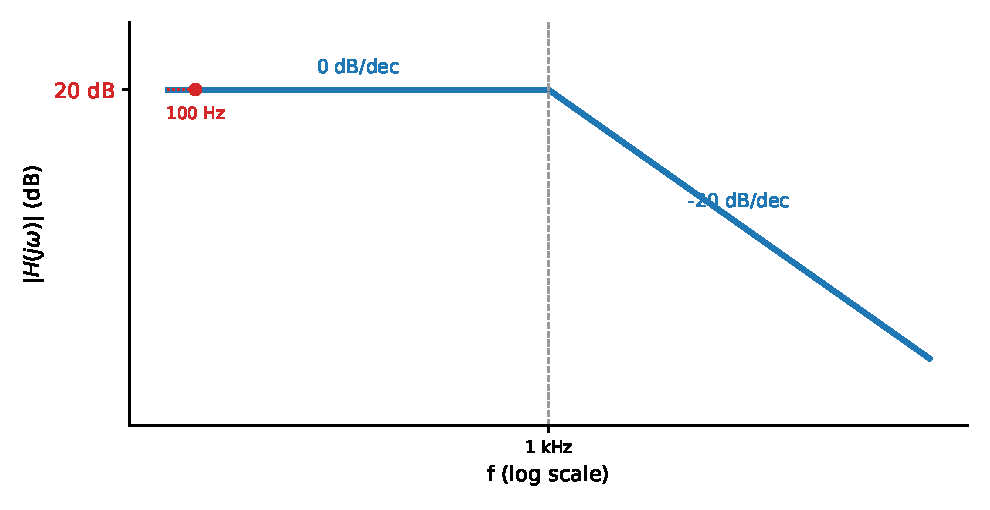
\includegraphics[width=\linewidth,height=5.6cm,keepaspectratio]{p01_plot}\end{center}
\end{probbox}

\begin{probbox}{Problem 2C.2 \hfill Easy}
Design a circuit with op-amps, resistors and capacitors whose transfer function $H(s)=\dfrac{V_o(s)}{V_i(s)}$ has the straight-line magnitude Bode plot below ($K>0$, no right-half-plane poles or zeros; use the design rules stated at the top of this set). Then find the steady-state output $V_o(t)$ for $V_i(t) = 0.2\sin\left(2\pi\cdot 100\,t\right)$.
\begin{center}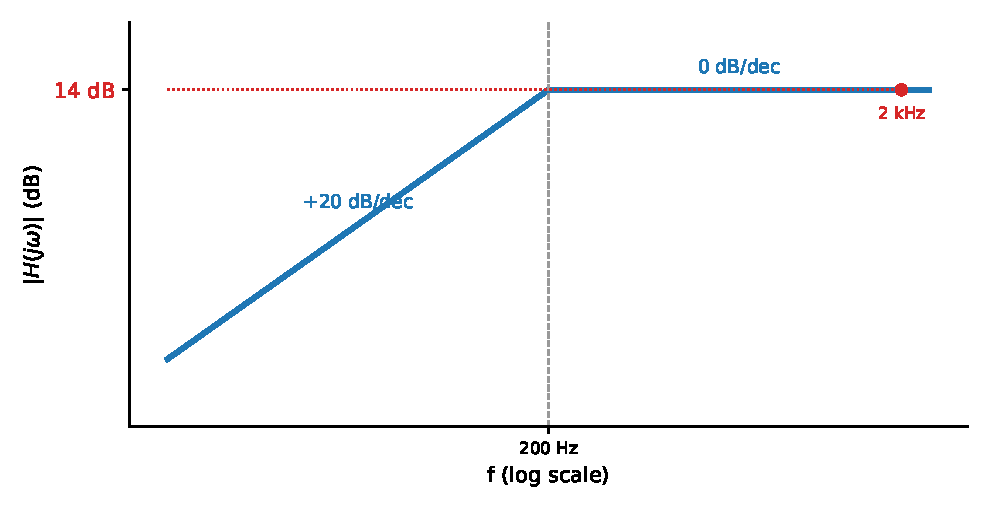
\includegraphics[width=\linewidth,height=5.6cm,keepaspectratio]{p02_plot}\end{center}
\end{probbox}

\begin{probbox}{Problem 2C.3 \hfill Easy}
Design a circuit with op-amps, resistors and capacitors whose transfer function $H(s)=\dfrac{V_o(s)}{V_i(s)}$ has the straight-line magnitude Bode plot below ($K>0$, no right-half-plane poles or zeros; use the design rules stated at the top of this set). Then find the steady-state output $V_o(t)$ for $V_i(t) = 1\cos\left(2\pi\cdot 10000\,t\right)$.
\begin{center}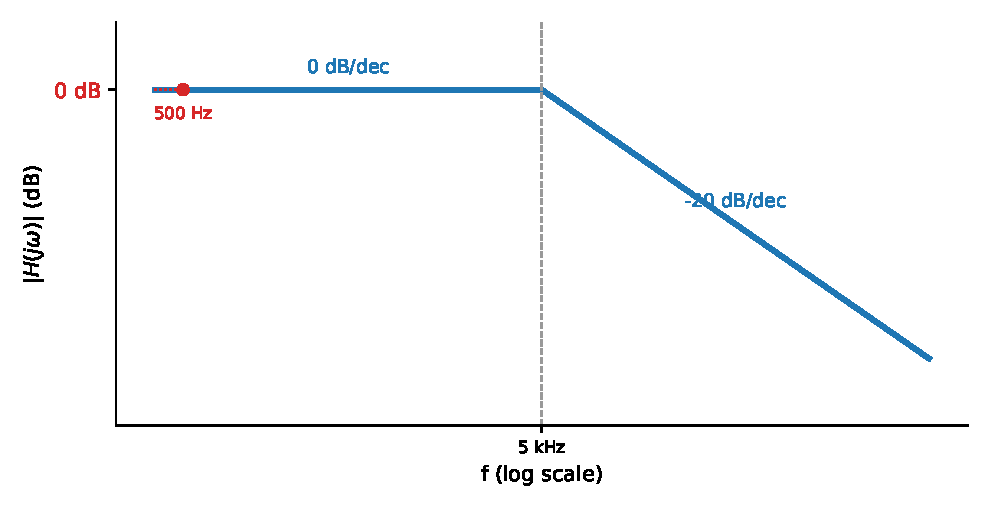
\includegraphics[width=\linewidth,height=5.6cm,keepaspectratio]{p03_plot}\end{center}
\end{probbox}

\begin{probbox}{Problem 2C.4 \hfill Easy}
Design a circuit with op-amps, resistors and capacitors whose transfer function $H(s)=\dfrac{V_o(s)}{V_i(s)}$ has the straight-line magnitude Bode plot below ($K>0$, no right-half-plane poles or zeros; use the design rules stated at the top of this set). Then find the steady-state output $V_o(t)$ for $V_i(t) = 0.05\sin\left(2\pi\cdot 300\,t\right)$.
\begin{center}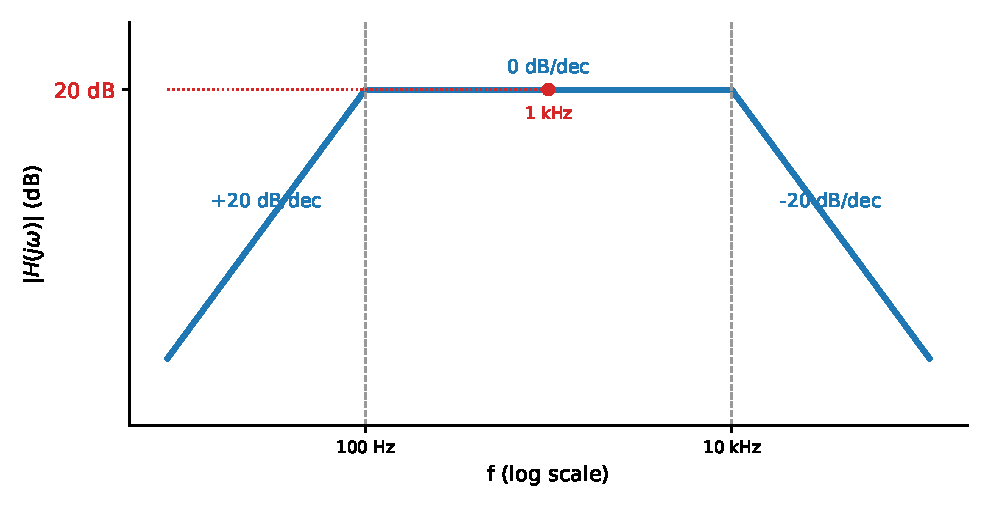
\includegraphics[width=\linewidth,height=5.6cm,keepaspectratio]{p04_plot}\end{center}
\end{probbox}

\begin{probbox}{Problem 2C.5 \hfill Easy}
Design a circuit with op-amps, resistors and capacitors whose transfer function $H(s)=\dfrac{V_o(s)}{V_i(s)}$ has the straight-line magnitude Bode plot below ($K>0$, no right-half-plane poles or zeros; use the design rules stated at the top of this set). Then find the steady-state output $V_o(t)$ for $V_i(t) = 0.1\sin\left(2\pi\cdot 500\,t\right)$.
\begin{center}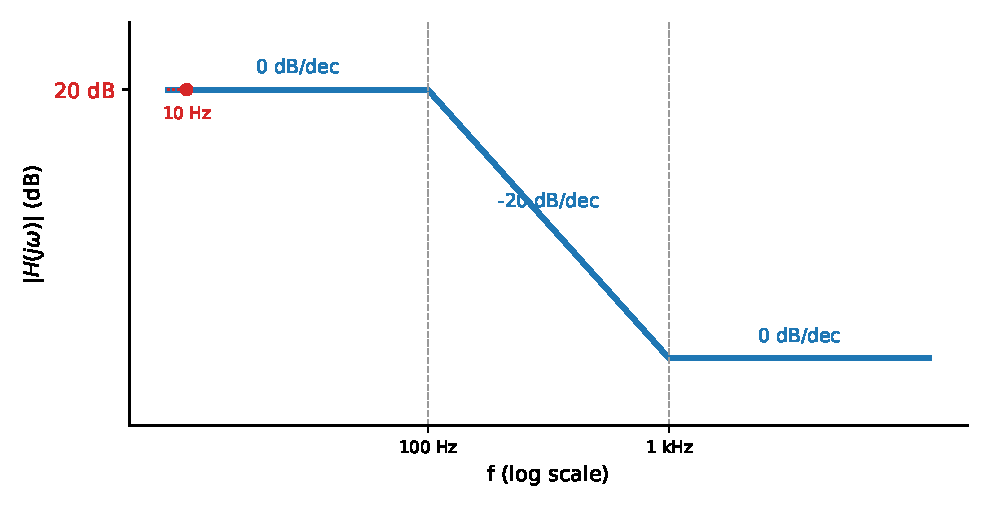
\includegraphics[width=\linewidth,height=5.6cm,keepaspectratio]{p05_plot}\end{center}
\end{probbox}

\begin{probbox}{Problem 2C.6 \hfill Easy}
Design a circuit with op-amps, resistors and capacitors whose transfer function $H(s)=\dfrac{V_o(s)}{V_i(s)}$ has the straight-line magnitude Bode plot below ($K>0$, no right-half-plane poles or zeros; use the design rules stated at the top of this set). Then find the steady-state output $V_o(t)$ for $V_i(t) = 0.5\sin\left(2\pi\cdot 3000\,t\right)$.
\begin{center}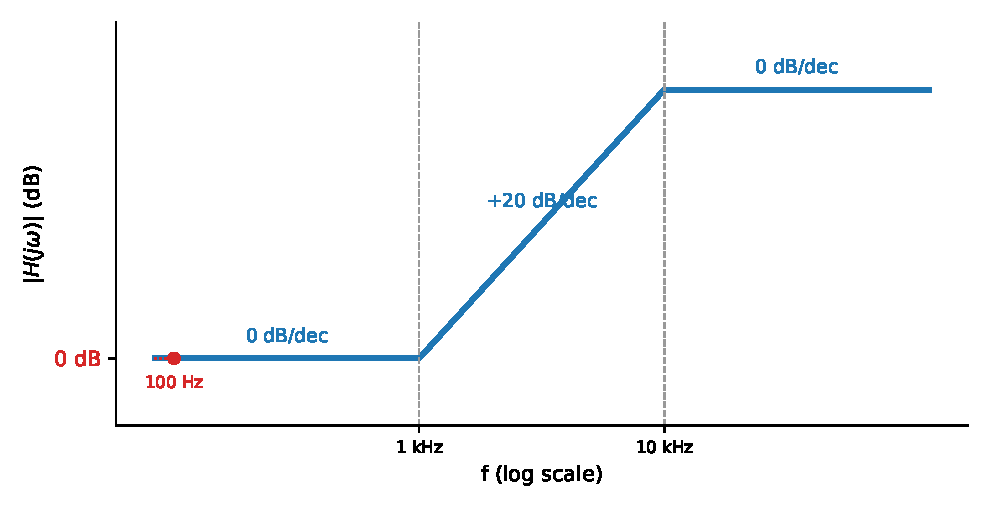
\includegraphics[width=\linewidth,height=5.6cm,keepaspectratio]{p06_plot}\end{center}
\end{probbox}

\subsection*{Medium problems}
\begin{probbox}{Problem 2C.7 \hfill Medium}
Design a circuit with op-amps, resistors and capacitors whose transfer function $H(s)=\dfrac{V_o(s)}{V_i(s)}$ has the straight-line magnitude Bode plot below ($K>0$, no right-half-plane poles or zeros; use the design rules stated at the top of this set). Then find the steady-state output $V_o(t)$ for $V_i(t) = 0.05\sin\left(2\pi\cdot 5000\,t\right)$.
\begin{center}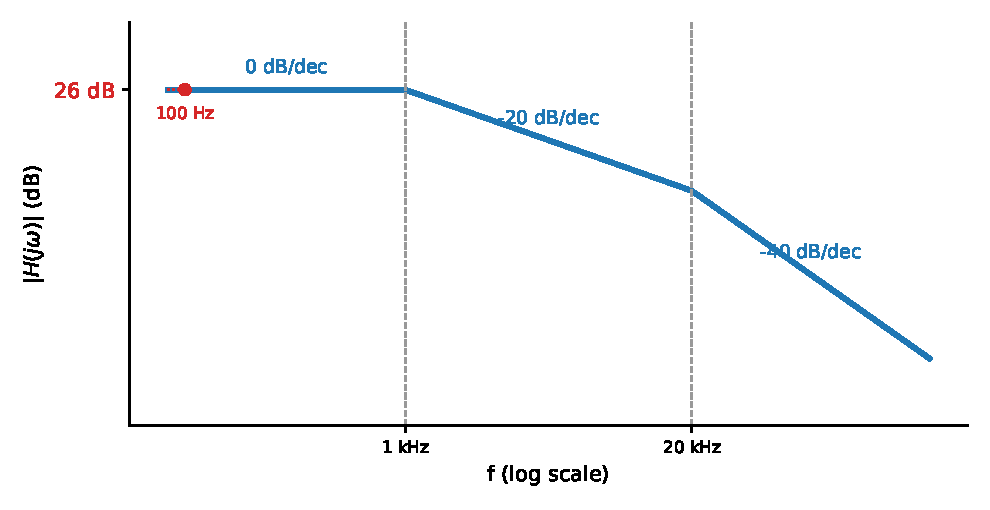
\includegraphics[width=\linewidth,height=5.6cm,keepaspectratio]{p07_plot}\end{center}
\end{probbox}

\begin{probbox}{Problem 2C.8 \hfill Medium}
Design a circuit with op-amps, resistors and capacitors whose transfer function $H(s)=\dfrac{V_o(s)}{V_i(s)}$ has the straight-line magnitude Bode plot below ($K>0$, no right-half-plane poles or zeros; use the design rules stated at the top of this set). Then find the steady-state output $V_o(t)$ for $V_i(t) = 0.1\sin\left(2\pi\cdot 300\,t\right)$.
\begin{center}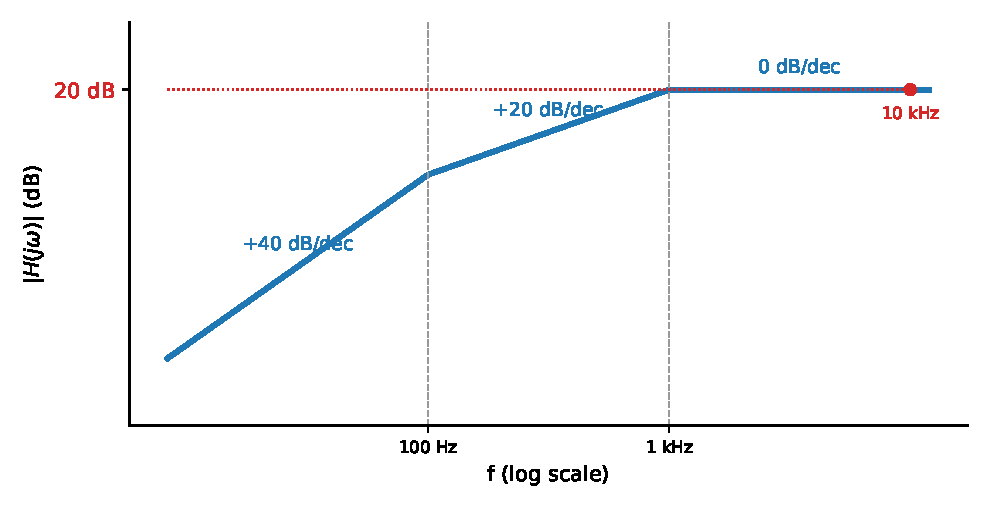
\includegraphics[width=\linewidth,height=5.6cm,keepaspectratio]{p08_plot}\end{center}
\end{probbox}

\begin{probbox}{Problem 2C.9 \hfill Medium}
Design a circuit with op-amps, resistors and capacitors whose transfer function $H(s)=\dfrac{V_o(s)}{V_i(s)}$ has the straight-line magnitude Bode plot below ($K>0$, no right-half-plane poles or zeros; use the design rules stated at the top of this set). Then find the steady-state output $V_o(t)$ for $V_i(t) = 0.2\sin\left(2\pi\cdot 1000\,t\right)$.
\begin{center}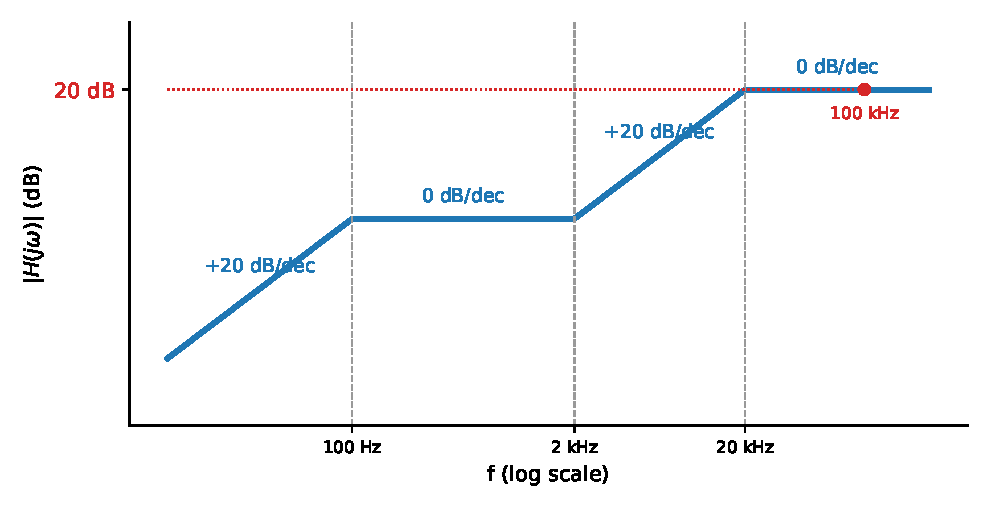
\includegraphics[width=\linewidth,height=5.6cm,keepaspectratio]{p09_plot}\end{center}
\end{probbox}

\begin{probbox}{Problem 2C.10 \hfill Medium}
Design a circuit with op-amps, resistors and capacitors whose transfer function $H(s)=\dfrac{V_o(s)}{V_i(s)}$ has the straight-line magnitude Bode plot below ($K>0$, no right-half-plane poles or zeros; use the design rules stated at the top of this set). Then find the steady-state output $V_o(t)$ for $V_i(t) = 0.2\sin\left(2\pi\cdot 2000\,t\right)$.
\begin{center}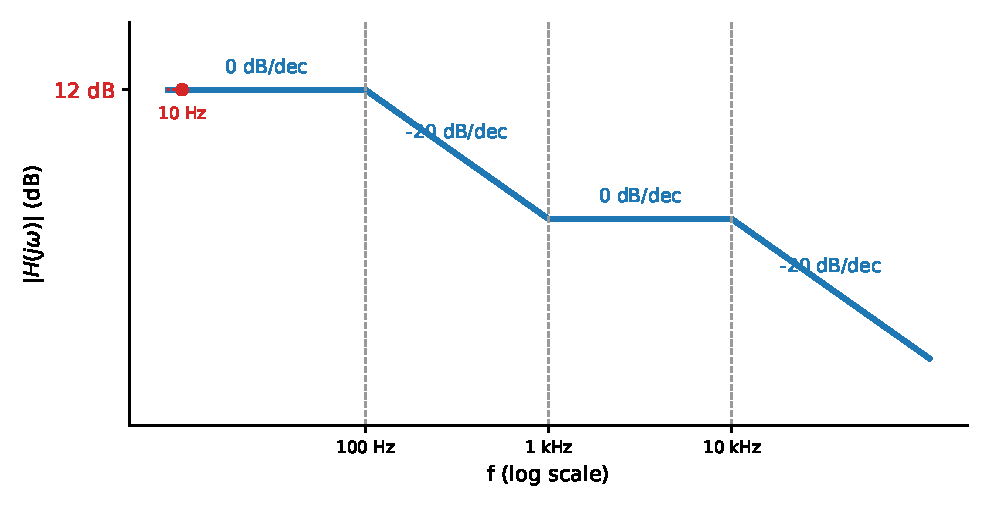
\includegraphics[width=\linewidth,height=5.6cm,keepaspectratio]{p10_plot}\end{center}
\end{probbox}

\begin{probbox}{Problem 2C.11 \hfill Medium}
Design a circuit with op-amps, resistors and capacitors whose transfer function $H(s)=\dfrac{V_o(s)}{V_i(s)}$ has the straight-line magnitude Bode plot below ($K>0$, no right-half-plane poles or zeros; use the design rules stated at the top of this set). Then find the steady-state output $V_o(t)$ for $V_i(t) = 0.1\sin\left(2\pi\cdot 5000\,t\right)$.
\begin{center}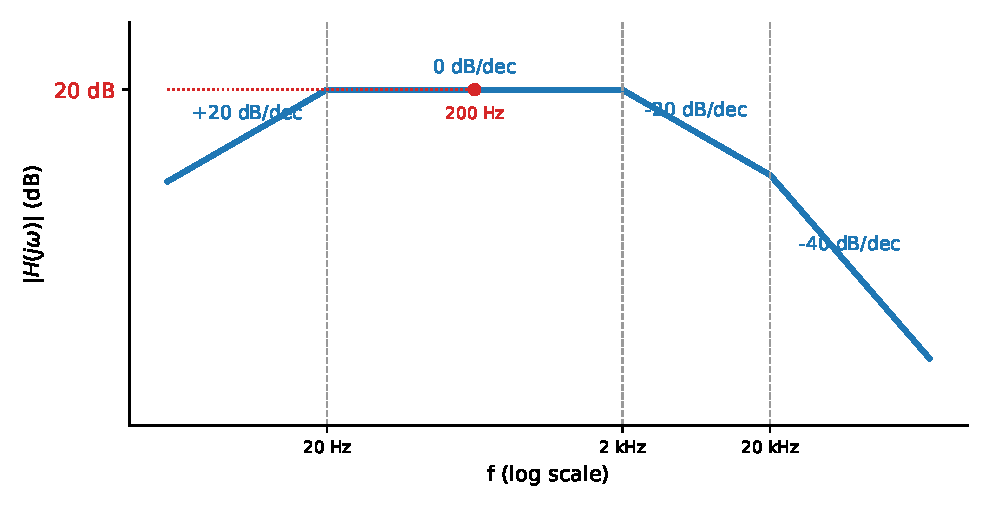
\includegraphics[width=\linewidth,height=5.6cm,keepaspectratio]{p11_plot}\end{center}
\end{probbox}

\begin{probbox}{Problem 2C.12 \hfill Medium}
Design a circuit with op-amps, resistors and capacitors whose transfer function $H(s)=\dfrac{V_o(s)}{V_i(s)}$ has the straight-line magnitude Bode plot below ($K>0$, no right-half-plane poles or zeros; use the design rules stated at the top of this set). Then find the steady-state output $V_o(t)$ for $V_i(t) = 1\sin\left(2\pi\cdot 1000\,t+\frac{\pi}{4}\right)$.
\begin{center}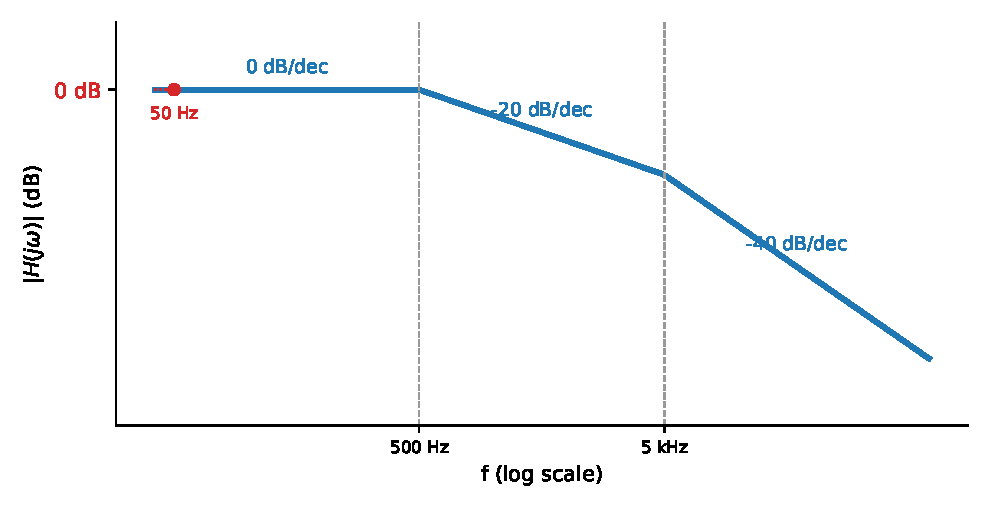
\includegraphics[width=\linewidth,height=5.6cm,keepaspectratio]{p12_plot}\end{center}
\end{probbox}

\subsection*{Hard problems}
\begin{probbox}{Problem 2C.13 \hfill Hard}
Design a circuit with op-amps, resistors and capacitors whose transfer function $H(s)=\dfrac{V_o(s)}{V_i(s)}$ has the straight-line magnitude Bode plot below ($K>0$, no right-half-plane poles or zeros; use the design rules stated at the top of this set). Then find the steady-state output $V_o(t)$ for $V_i(t) = 0.01\sin\left(2\pi\cdot 2000\,t\right)$.
\begin{center}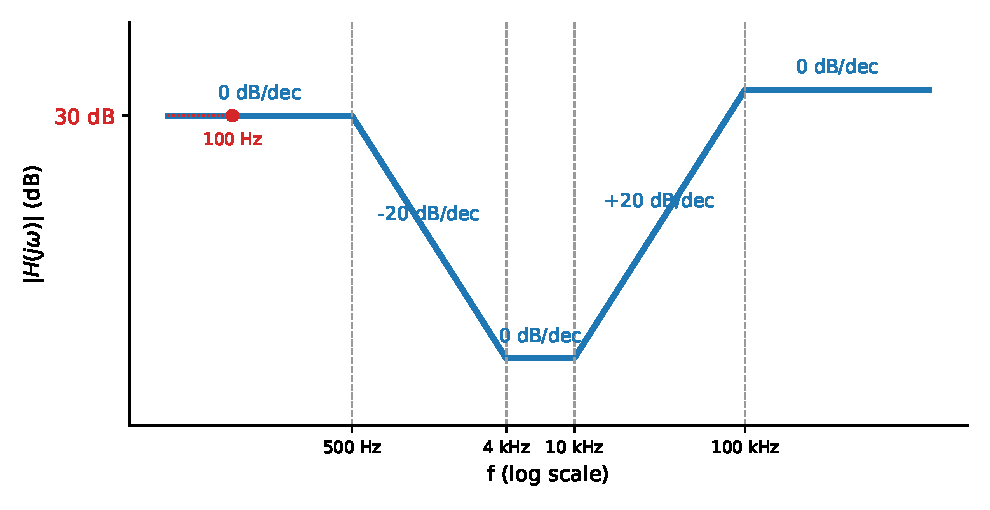
\includegraphics[width=\linewidth,height=5.6cm,keepaspectratio]{p13_plot}\end{center}
\end{probbox}

\begin{probbox}{Problem 2C.14 \hfill Hard}
Design a circuit with op-amps, resistors and capacitors whose transfer function $H(s)=\dfrac{V_o(s)}{V_i(s)}$ has the straight-line magnitude Bode plot below ($K>0$, no right-half-plane poles or zeros; use the design rules stated at the top of this set). Then find the steady-state output $V_o(t)$ for $V_i(t) = 0.3\sin\left(2\pi\cdot 10000\,t\right)$.
\begin{center}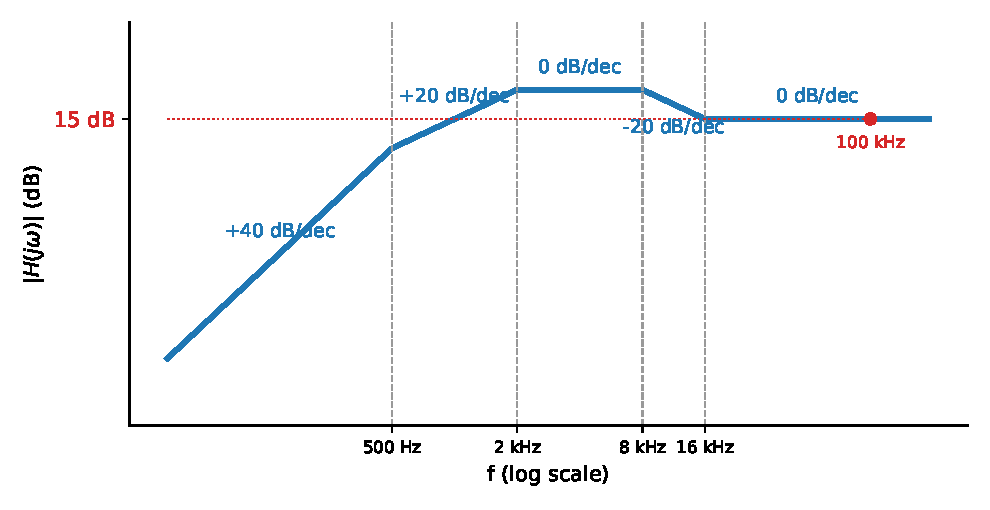
\includegraphics[width=\linewidth,height=5.6cm,keepaspectratio]{p14_plot}\end{center}
\end{probbox}

\begin{probbox}{Problem 2C.15 \hfill Hard}
Design a circuit with op-amps, resistors and capacitors whose transfer function $H(s)=\dfrac{V_o(s)}{V_i(s)}$ has the straight-line magnitude Bode plot below ($K>0$, no right-half-plane poles or zeros; use the design rules stated at the top of this set). Then find the steady-state output $V_o(t)$ for $V_i(t) = 0.2\sin\left(2\pi\cdot 2000\,t+\frac{\pi}{3}\right)$.
\begin{center}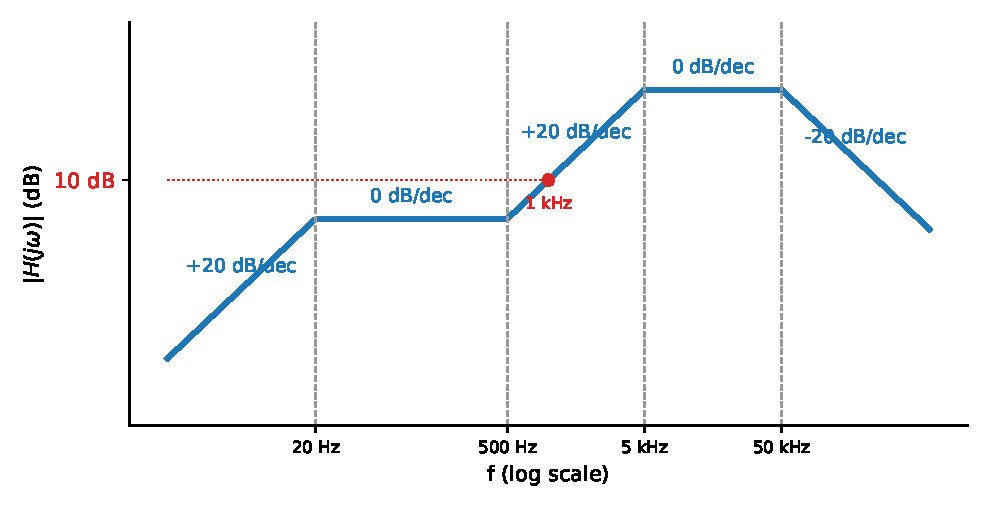
\includegraphics[width=\linewidth,height=5.6cm,keepaspectratio]{p15_plot}\end{center}
\end{probbox}

\begin{probbox}{Problem 2C.16 \hfill Hard}
Design a circuit with op-amps, resistors and capacitors whose transfer function $H(s)=\dfrac{V_o(s)}{V_i(s)}$ has the straight-line magnitude Bode plot below ($K>0$, no right-half-plane poles or zeros; use the design rules stated at the top of this set). Then find the steady-state output $V_o(t)$ for $V_i(t) = 0.1\sin\left(2\pi\cdot 300\,t\right)$.
\begin{center}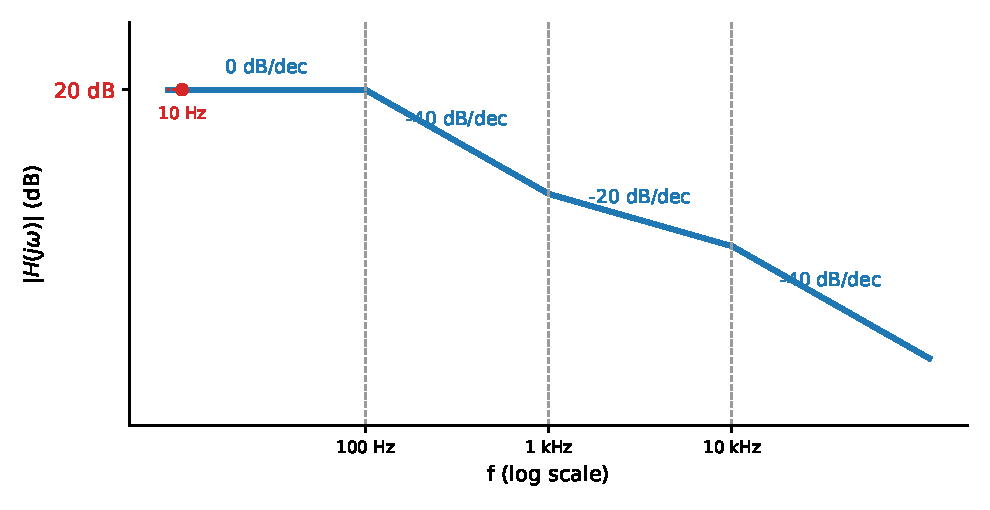
\includegraphics[width=\linewidth,height=5.6cm,keepaspectratio]{p16_plot}\end{center}
\end{probbox}

\begin{probbox}{Problem 2C.17 \hfill Hard}
Design a circuit with op-amps, resistors and capacitors whose transfer function $H(s)=\dfrac{V_o(s)}{V_i(s)}$ has the straight-line magnitude Bode plot below ($K>0$, no right-half-plane poles or zeros; use the design rules stated at the top of this set). Then find the steady-state output $V_o(t)$ for $V_i(t) = 0.05\cos\left(2\pi\cdot 1000\,t-\frac{\pi}{6}\right)$.
\begin{center}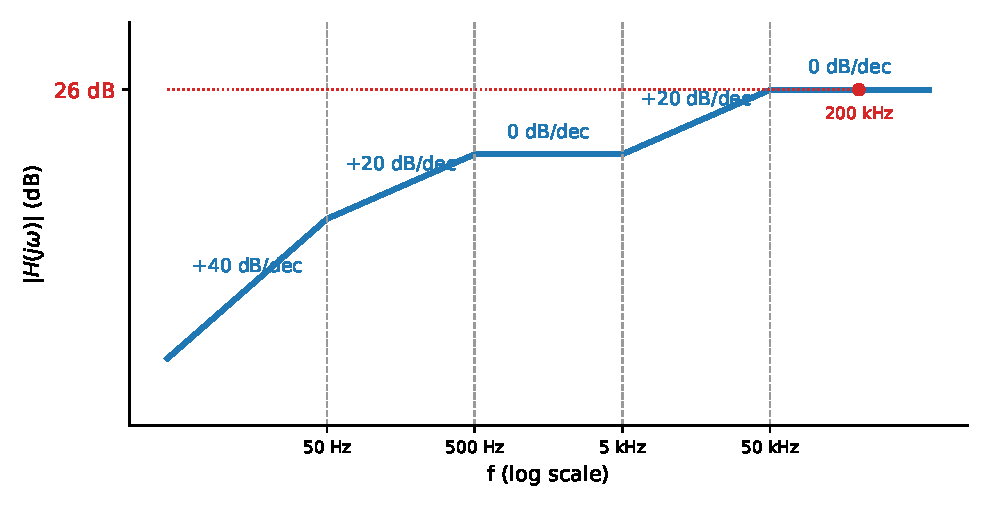
\includegraphics[width=\linewidth,height=5.6cm,keepaspectratio]{p17_plot}\end{center}
\end{probbox}

\begin{probbox}{Problem 2C.18 \hfill Hard}
Design a circuit with op-amps, resistors and capacitors whose transfer function $H(s)=\dfrac{V_o(s)}{V_i(s)}$ has the straight-line magnitude Bode plot below ($K>0$, no right-half-plane poles or zeros; use the design rules stated at the top of this set). Then find the steady-state output $V_o(t)$ for $V_i(t) = 0.5\sin\left(2\pi\cdot 3000\,t\right)$.
\begin{center}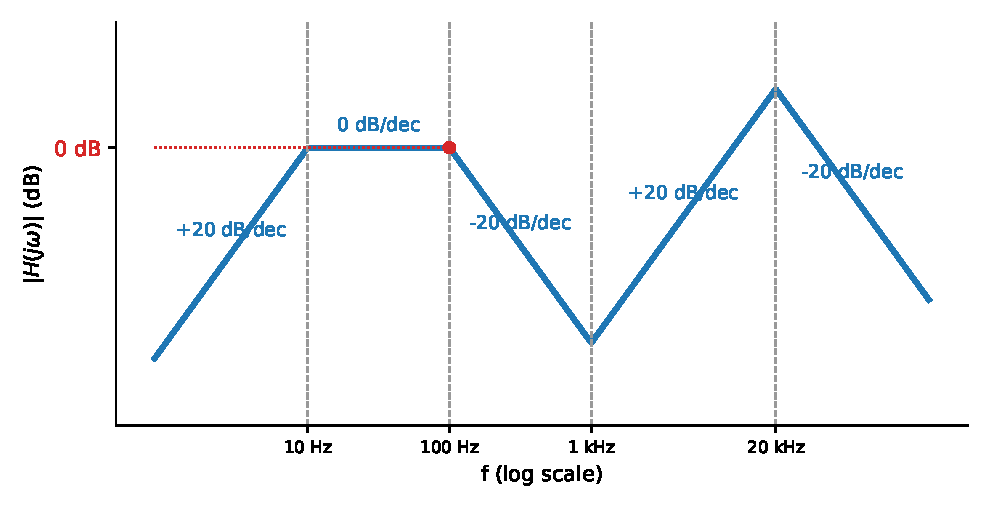
\includegraphics[width=\linewidth,height=5.6cm,keepaspectratio]{p18_plot}\end{center}
\end{probbox}

\newpage
\section*{Solutions}
Every solution follows the steps of the Lecture-2 pipeline card.
\newpage
\subsection*{Solution 2C.1 \hfill Easy}
\begin{center}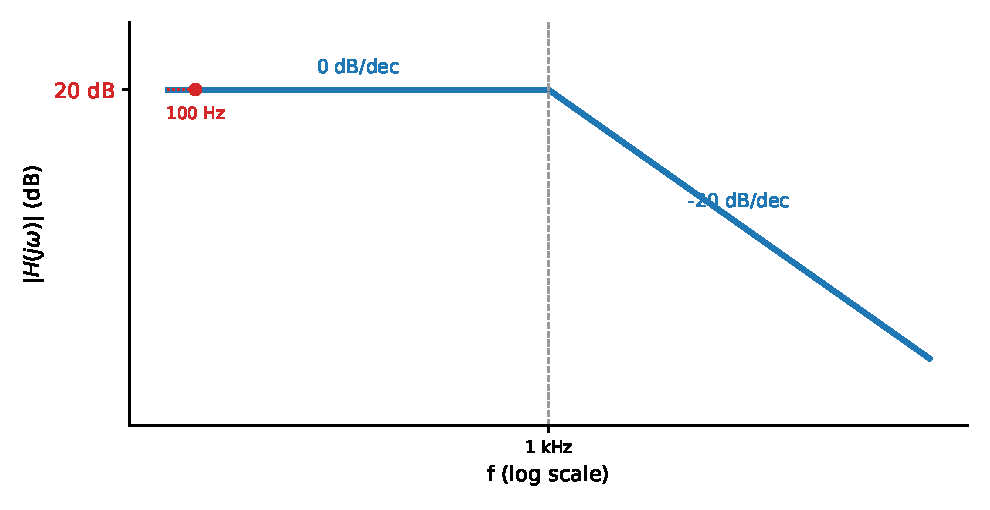
\includegraphics[width=\linewidth,height=5cm,keepaspectratio]{p01_plot}\end{center}
\solstep{1}{Read the corners and slopes}Go left to right along the plot and write down the slope of every straight segment. At each corner frequency the slope changes by a multiple of 20\,dB/dec: every $-20$ is one pole, every $+20$ is one zero (tool T6 read backwards).\begin{center}\renewcommand{\arraystretch}{1.35}
\begin{tabular}{ccccl}
\toprule
corner $f_c$ & slope before & slope after & change & meaning \\
\midrule
1 kHz & $0$ & $-20$ & $-20$ & one pole at $f_c$ \\
\bottomrule
\end{tabular}\end{center}

\solstep{2}{Starting slope $\Rightarrow$ factors of $s$}The plot starts \emph{flat} (0\,dB/dec), so there is no factor $s$ in the numerator: every pole is written as $\frac{1}{1+s/p}$ and every zero as $\left(1+\frac{s}{z}\right)$, which are all $\approx1$ (0\,dB) at low frequency. Every corner is an angular frequency $\omega_c=2\pi f_c$.
\solstep{3}{Assemble $H(s)$}Put one factor per pole/zero in front of an unknown constant $K$:\[
H(s) = K\,\dfrac{1}{1+\dfrac{s}{2\pi\cdot 1\mathrm{k}}}
\]

\solstep{4}{Find $K$ from the marked level}The plot marks the level $20$\,dB at $f=$\,100 Hz. On the straight-line plot every factor is either exactly 0\,dB (where it is $\approx1$) or a $\pm20$\,dB/dec line, so evaluate the \emph{asymptote} of each factor at that frequency (the level of a line with slope $\pm20$\,dB/dec is $\pm20\log_{10}(f/f_c)$):\begin{center}\renewcommand{\arraystretch}{1.35}
\begin{tabular}{cccc}
\toprule
factor & $f_c$ & at $f=$\,100 Hz & asymptote (dB) \\
\midrule
$\rule[-1.7em]{0pt}{4em}\dfrac{1}{1+\dfrac{s}{2\pi\cdot 1\mathrm{k}}}$ & 1 kHz & $f<f_c$: $\approx 1$ & $0$ \\
\textbf{sum} &  &  & $\mathbf{0}$ \\
\bottomrule
\end{tabular}\end{center}
The dB values of the factors \emph{add} (magnitudes multiply), so\[
20\log_{10}K = 20 - (0) = 20\ \mathrm{dB}\quad\Rightarrow\quad K = 10^{20/20} = 10
\]

So\[
\boxed{H(s) = 10\,\dfrac{1}{1+\dfrac{s}{2\pi\cdot 1\mathrm{k}}}}
\]


\solstep{5}{Split $H(s)$ into op-amp stages}Every inverting stage of the form $-\frac{Z_f}{Z_{in}}$ with $Z_{in}$, $Z_f$ made of one R and at most one C realizes \emph{one} pole, optionally with one zero or one $s$ (tool T2). Pair each zero with a low-pass pole (pole-zero stage), each $\frac{s}{s+p}$ with a remaining low-pass pole (band-pass stage), and give every leftover factor its own stage. Put all of $|K|$ into the first stage. Each stage inverts, so with an odd number of stages add a unity-gain inverter to make $K>0$.\begin{center}\renewcommand{\arraystretch}{1.35}
\begin{tabular}{cccl}
\toprule
stage & gain $\frac{R_2}{R_1}$ & factor(s) realized & block \\
\midrule
U1 & $10$ & $\rule[-1.4em]{0pt}{3.4em}\dfrac{1}{1+\frac{s}{2\pi\cdot 1\mathrm{k}}}$ & low-pass: $Z_{in}=R$, $Z_f=R\parallel C$ \\
U2 & $1$ & $\rule[-1.4em]{0pt}{3.4em}1$ & unity inverter (fixes the sign) \\
\bottomrule
\end{tabular}\end{center}

\solstep{6}{Component values}Use $R_1 = 10\,\mathrm{k}\Omega$ at the input of every stage (any convenient value works; it only scales the other parts). The corner of a factor $1+s/\omega_c$ is matched by $RC = 1/\omega_c$ (corners in rad/s).\begin{enumerate}[leftmargin=*,itemsep=2pt]
\item U1: choose $R_{1} = 10\,\mathrm{k}\Omega$, then match the stage formula $-\frac{R_{2}}{R_{1}}\cdot\frac{1}{1+sR_{2}C_{1}}$ to the factors:\[
R_{2} = 10\,R_{1} = 100\,\mathrm{k}\Omega,\qquad C_{1} = \frac{1}{6280\,R_{2}} = 1.59\,\mathrm{n}\mathrm{F}
\]

\item U2: $R_{3} = R_{4} = 10\,\mathrm{k}\Omega$ (gain $-1$).
\end{enumerate}

\solstep{7}{Check and steady-state output}The designed circuit:\begin{center}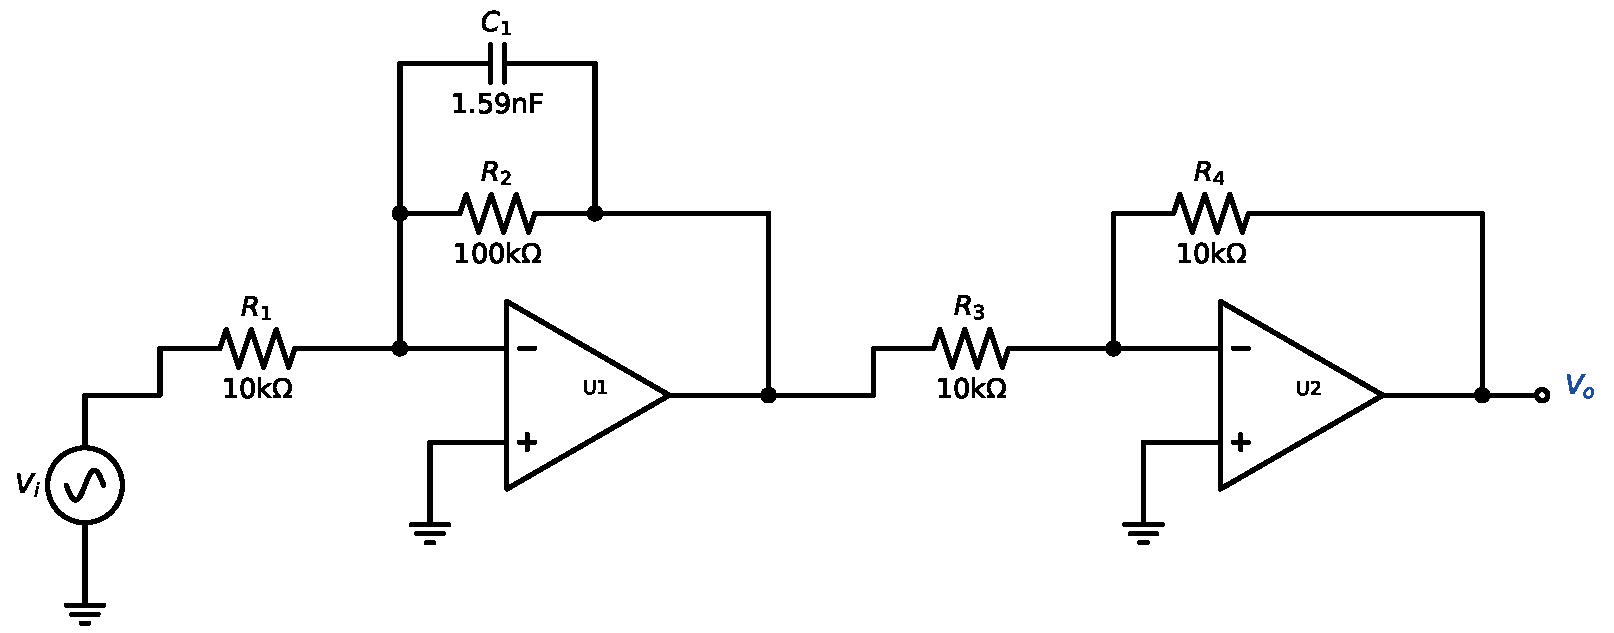
\includegraphics[width=\linewidth,height=5.5cm,keepaspectratio]{p01_design}\end{center}
Check: the stage gains multiply to $(-1)^{2}\cdot10\cdot(\text{factors}) = H(s)$; an independent nodal solve of this circuit reproduces $H(s)$ at every frequency. (Standard-value resistors and capacitors would move the corners slightly.)

The input is $V_i(t) = 0.1\sin\left(2\pi\cdot 2000\,t\right)$, so $\omega_{in} = 2\pi\cdot 2000 = 12600$\,rad/s. Put $s=j\omega_{in}$ in each factor (tool T5): magnitudes multiply, angles add.
{\small Rules: $\left|\frac{s}{s+p}\right| = \frac{\omega}{\sqrt{\omega^2+p^2}}$, $\angle = \frac{\pi}{2}-\tan^{-1}\frac{\omega}{p}$;\quad $\left|\frac{1}{1+s/p}\right| = \frac{1}{\sqrt{1+(\omega/p)^2}}$, $\angle = -\tan^{-1}\frac{\omega}{p}$;\quad $\left|1+\frac{s}{z}\right| = \sqrt{1+(\omega/z)^2}$, $\angle = \tan^{-1}\frac{\omega}{z}$;\quad a negative $K$ adds $-\pi$.}
\begin{center}\renewcommand{\arraystretch}{1.35}
\begin{tabular}{ccc}
\toprule
factor & magnitude & angle (rad) \\
\midrule
$10$ & $10$ & $0$ \\
$\rule[-1.7em]{0pt}{4em}\dfrac{1}{1+\dfrac{s}{2\pi\cdot 1\mathrm{k}}}$ & $0.4472$ & $-1.11$ \\
\textbf{total} & $\mathbf{4.472}$ (product) & $\mathbf{-1.11}$ (sum) \\
\bottomrule
\end{tabular}\end{center}

\begin{align*}
|H(j\omega_{in})| &= 4.47, \qquad \angle H(j\omega_{in}) = -1.11\ \mathrm{rad} \\
v_{o,ac}(t) &= 4.47\times 0.1\,\sin\left(2\pi\cdot 2000\,t - 1.11\right) = 0.447\,\sin\left(2\pi\cdot 2000\,t - 1.11\right)
\end{align*}

\[
\boxed{V_o(t) = 0.447\,\sin\left(2\pi\cdot 2000\,t - 1.11\right)\ \mathrm{V}}
\]

\begin{ansbox}
$H(s) = 10\,\dfrac{1}{1+\dfrac{s}{2\pi\cdot 1\mathrm{k}}}$\\[4pt]
U1: R1 = 10k$\Omega$, R2 = 100k$\Omega$, C1 = 1.59nF\\
U2: R3 = 10k$\Omega$, R4 = 10k$\Omega$\\[4pt]
$V_o(t) = 0.447\,\sin\left(2\pi\cdot 2000\,t - 1.11\right)\ \mathrm{V}$
\end{ansbox}

\newpage
\subsection*{Solution 2C.2 \hfill Easy}
\begin{center}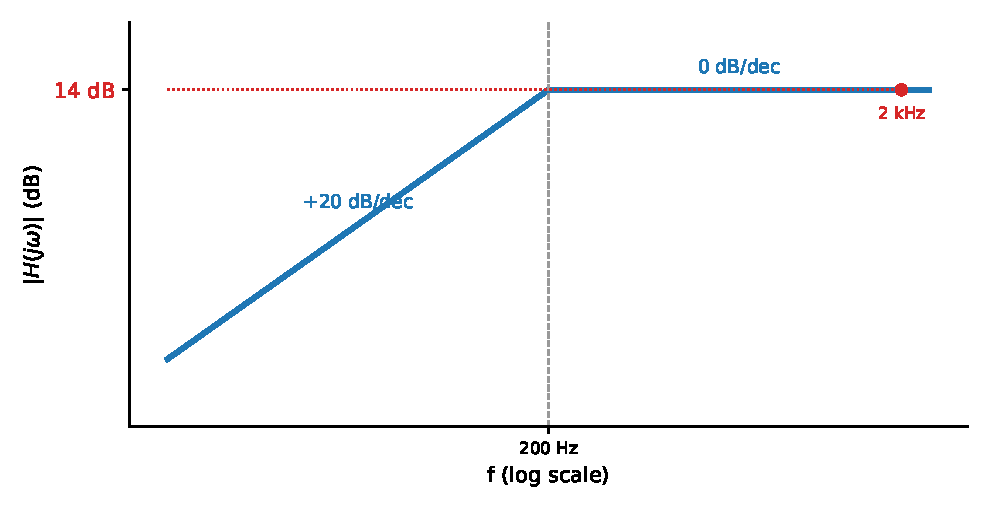
\includegraphics[width=\linewidth,height=5cm,keepaspectratio]{p02_plot}\end{center}
\solstep{1}{Read the corners and slopes}Go left to right along the plot and write down the slope of every straight segment. At each corner frequency the slope changes by a multiple of 20\,dB/dec: every $-20$ is one pole, every $+20$ is one zero (tool T6 read backwards).\begin{center}\renewcommand{\arraystretch}{1.35}
\begin{tabular}{ccccl}
\toprule
corner $f_c$ & slope before & slope after & change & meaning \\
\midrule
200 Hz & $+20$ & $0$ & $-20$ & one pole at $f_c$ \\
\bottomrule
\end{tabular}\end{center}

\solstep{2}{Starting slope $\Rightarrow$ factors of $s$}The plot starts with a slope of $+20$\,dB/dec, i.e. $|H|\propto\omega^1$ at low frequency: the numerator contains $s$. As in class, pair each $s$ with one of the \emph{lowest} poles (200 Hz) as $\frac{s}{s+p}$: such a factor rises at $+20$\,dB/dec below $p$ and is $\approx1$ (0\,dB) above it. The remaining poles are written $\frac{1}{1+s/p}$ and the zeros $\left(1+\frac{s}{z}\right)$. Every corner is an angular frequency $\omega_c=2\pi f_c$.
\solstep{3}{Assemble $H(s)$}Put one factor per pole/zero in front of an unknown constant $K$:\[
H(s) = K\,\dfrac{s}{s+2\pi\cdot 200}
\]

\solstep{4}{Find $K$ from the marked level}The plot marks the level $14$\,dB at $f=$\,2 kHz. On the straight-line plot every factor is either exactly 0\,dB (where it is $\approx1$) or a $\pm20$\,dB/dec line, so evaluate the \emph{asymptote} of each factor at that frequency (the level of a line with slope $\pm20$\,dB/dec is $\pm20\log_{10}(f/f_c)$):\begin{center}\renewcommand{\arraystretch}{1.35}
\begin{tabular}{cccc}
\toprule
factor & $f_c$ & at $f=$\,2 kHz & asymptote (dB) \\
\midrule
$\rule[-1.1em]{0pt}{2.8em}\dfrac{s}{s+2\pi\cdot 200}$ & 200 Hz & $f>f_c$: $\approx 1$ & $0$ \\
\textbf{sum} &  &  & $\mathbf{0}$ \\
\bottomrule
\end{tabular}\end{center}
The dB values of the factors \emph{add} (magnitudes multiply), so\[
20\log_{10}K = 14 - (0) = 14\ \mathrm{dB}\quad\Rightarrow\quad K = 10^{14/20} = 5.01
\]

So\[
\boxed{H(s) = 5.01\,\dfrac{s}{s+2\pi\cdot 200}}
\]


\solstep{5}{Split $H(s)$ into op-amp stages}Every inverting stage of the form $-\frac{Z_f}{Z_{in}}$ with $Z_{in}$, $Z_f$ made of one R and at most one C realizes \emph{one} pole, optionally with one zero or one $s$ (tool T2). Pair each zero with a low-pass pole (pole-zero stage), each $\frac{s}{s+p}$ with a remaining low-pass pole (band-pass stage), and give every leftover factor its own stage. Put all of $|K|$ into the first stage. Each stage inverts, so with an odd number of stages add a unity-gain inverter to make $K>0$.\begin{center}\renewcommand{\arraystretch}{1.35}
\begin{tabular}{cccl}
\toprule
stage & gain $\frac{R_2}{R_1}$ & factor(s) realized & block \\
\midrule
U1 & $5.012$ & $\rule[-1.4em]{0pt}{3.4em}\dfrac{s}{s+2\pi\cdot 200}$ & high-pass: $Z_{in}=R+\frac{1}{sC}$, $Z_f=R$ \\
U2 & $1$ & $\rule[-1.4em]{0pt}{3.4em}1$ & unity inverter (fixes the sign) \\
\bottomrule
\end{tabular}\end{center}

\solstep{6}{Component values}Use $R_1 = 10\,\mathrm{k}\Omega$ at the input of every stage (any convenient value works; it only scales the other parts). The corner of a factor $1+s/\omega_c$ is matched by $RC = 1/\omega_c$ (corners in rad/s).\begin{enumerate}[leftmargin=*,itemsep=2pt]
\item U1: choose $R_{1} = 10\,\mathrm{k}\Omega$, then match the stage formula $-\frac{R_{2}}{R_{1}}\cdot\frac{s}{s+1/(R_{1}C_{1})}$ to the factors:\[
C_{1} = \frac{1}{1260\,R_{1}} = 79.6\,\mathrm{n}\mathrm{F},\qquad R_{2} = 5.012\,R_{1} = 50.1\,\mathrm{k}\Omega
\]

\item U2: $R_{3} = R_{4} = 10\,\mathrm{k}\Omega$ (gain $-1$).
\end{enumerate}

\solstep{7}{Check and steady-state output}The designed circuit:\begin{center}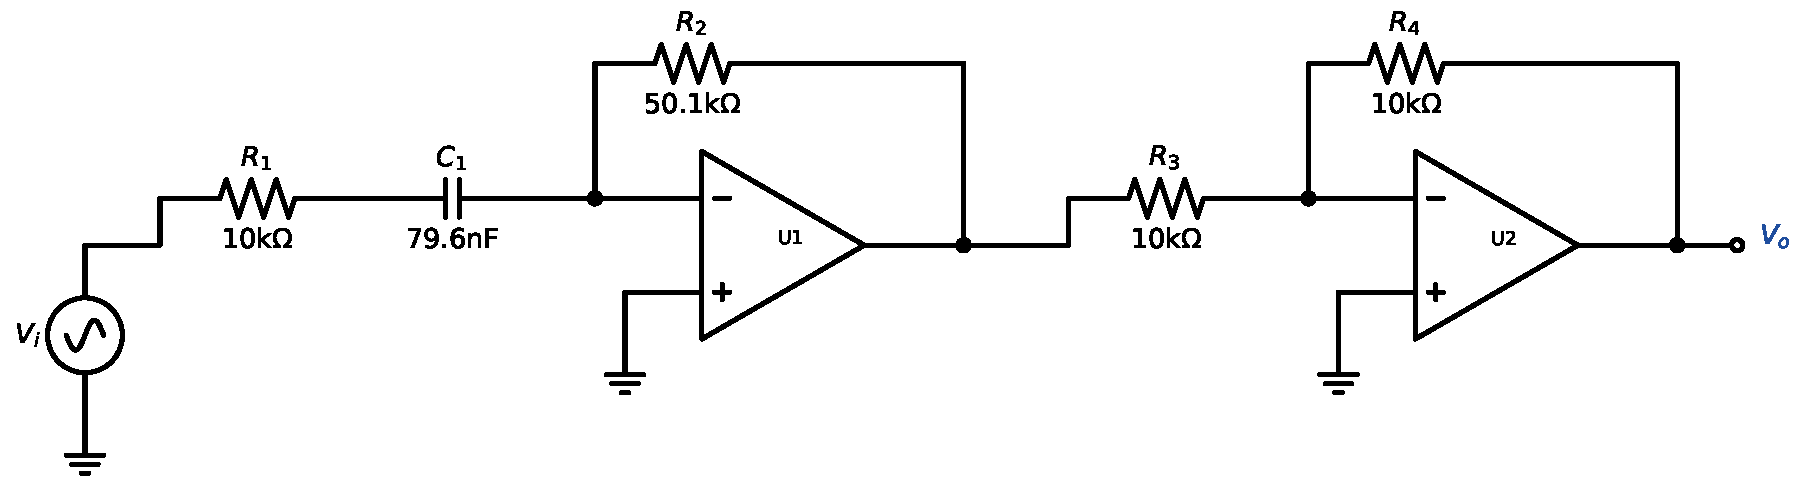
\includegraphics[width=\linewidth,height=5.5cm,keepaspectratio]{p02_design}\end{center}
Check: the stage gains multiply to $(-1)^{2}\cdot5.012\cdot(\text{factors}) = H(s)$; an independent nodal solve of this circuit reproduces $H(s)$ at every frequency. (Standard-value resistors and capacitors would move the corners slightly.)

The input is $V_i(t) = 0.2\sin\left(2\pi\cdot 100\,t\right)$, so $\omega_{in} = 2\pi\cdot 100 = 628$\,rad/s. Put $s=j\omega_{in}$ in each factor (tool T5): magnitudes multiply, angles add.
{\small Rules: $\left|\frac{s}{s+p}\right| = \frac{\omega}{\sqrt{\omega^2+p^2}}$, $\angle = \frac{\pi}{2}-\tan^{-1}\frac{\omega}{p}$;\quad $\left|\frac{1}{1+s/p}\right| = \frac{1}{\sqrt{1+(\omega/p)^2}}$, $\angle = -\tan^{-1}\frac{\omega}{p}$;\quad $\left|1+\frac{s}{z}\right| = \sqrt{1+(\omega/z)^2}$, $\angle = \tan^{-1}\frac{\omega}{z}$;\quad a negative $K$ adds $-\pi$.}
\begin{center}\renewcommand{\arraystretch}{1.35}
\begin{tabular}{ccc}
\toprule
factor & magnitude & angle (rad) \\
\midrule
$5.01$ & $5.012$ & $0$ \\
$\rule[-1.1em]{0pt}{2.8em}\dfrac{s}{s+2\pi\cdot 200}$ & $0.4472$ & $1.11$ \\
\textbf{total} & $\mathbf{2.241}$ (product) & $\mathbf{1.11}$ (sum) \\
\bottomrule
\end{tabular}\end{center}

\begin{align*}
|H(j\omega_{in})| &= 2.24, \qquad \angle H(j\omega_{in}) = 1.11\ \mathrm{rad} \\
v_{o,ac}(t) &= 2.24\times 0.2\,\sin\left(2\pi\cdot 100\,t + 1.11\right) = 0.448\,\sin\left(2\pi\cdot 100\,t + 1.11\right)
\end{align*}

\[
\boxed{V_o(t) = 0.448\,\sin\left(2\pi\cdot 100\,t + 1.11\right)\ \mathrm{V}}
\]

\begin{ansbox}
$H(s) = 5.01\,\dfrac{s}{s+2\pi\cdot 200}$\\[4pt]
U1: R1 = 10k$\Omega$, C1 = 79.6nF, R2 = 50.1k$\Omega$\\
U2: R3 = 10k$\Omega$, R4 = 10k$\Omega$\\[4pt]
$V_o(t) = 0.448\,\sin\left(2\pi\cdot 100\,t + 1.11\right)\ \mathrm{V}$
\end{ansbox}

\newpage
\subsection*{Solution 2C.3 \hfill Easy}
\begin{center}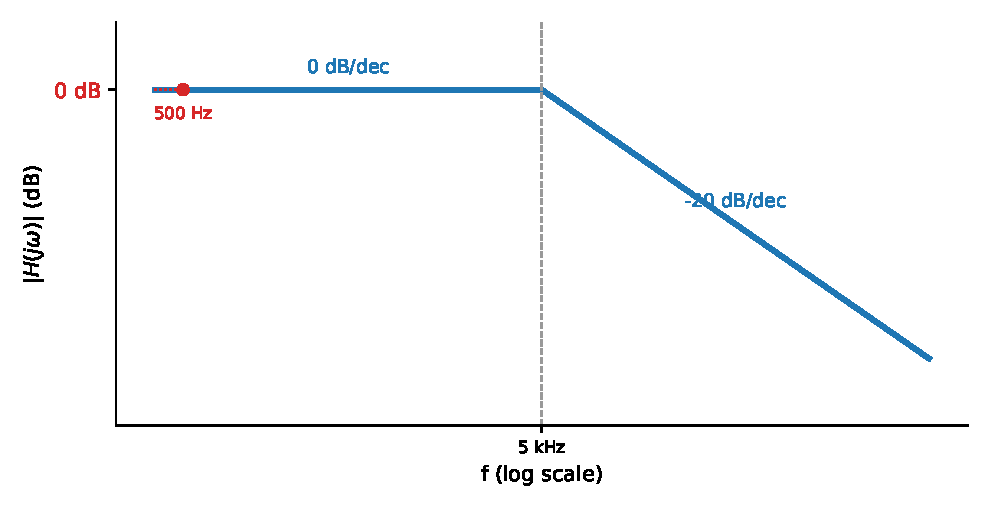
\includegraphics[width=\linewidth,height=5cm,keepaspectratio]{p03_plot}\end{center}
\solstep{1}{Read the corners and slopes}Go left to right along the plot and write down the slope of every straight segment. At each corner frequency the slope changes by a multiple of 20\,dB/dec: every $-20$ is one pole, every $+20$ is one zero (tool T6 read backwards).\begin{center}\renewcommand{\arraystretch}{1.35}
\begin{tabular}{ccccl}
\toprule
corner $f_c$ & slope before & slope after & change & meaning \\
\midrule
5 kHz & $0$ & $-20$ & $-20$ & one pole at $f_c$ \\
\bottomrule
\end{tabular}\end{center}

\solstep{2}{Starting slope $\Rightarrow$ factors of $s$}The plot starts \emph{flat} (0\,dB/dec), so there is no factor $s$ in the numerator: every pole is written as $\frac{1}{1+s/p}$ and every zero as $\left(1+\frac{s}{z}\right)$, which are all $\approx1$ (0\,dB) at low frequency. Every corner is an angular frequency $\omega_c=2\pi f_c$.
\solstep{3}{Assemble $H(s)$}Put one factor per pole/zero in front of an unknown constant $K$:\[
H(s) = K\,\dfrac{1}{1+\dfrac{s}{2\pi\cdot 5\mathrm{k}}}
\]

\solstep{4}{Find $K$ from the marked level}The plot marks the level $0$\,dB at $f=$\,500 Hz. On the straight-line plot every factor is either exactly 0\,dB (where it is $\approx1$) or a $\pm20$\,dB/dec line, so evaluate the \emph{asymptote} of each factor at that frequency (the level of a line with slope $\pm20$\,dB/dec is $\pm20\log_{10}(f/f_c)$):\begin{center}\renewcommand{\arraystretch}{1.35}
\begin{tabular}{cccc}
\toprule
factor & $f_c$ & at $f=$\,500 Hz & asymptote (dB) \\
\midrule
$\rule[-1.7em]{0pt}{4em}\dfrac{1}{1+\dfrac{s}{2\pi\cdot 5\mathrm{k}}}$ & 5 kHz & $f<f_c$: $\approx 1$ & $0$ \\
\textbf{sum} &  &  & $\mathbf{0}$ \\
\bottomrule
\end{tabular}\end{center}
The dB values of the factors \emph{add} (magnitudes multiply), so\[
20\log_{10}K = 0 - (0) = 0\ \mathrm{dB}\quad\Rightarrow\quad K = 10^{0/20} = 1
\]

So\[
\boxed{H(s) = 1\,\dfrac{1}{1+\dfrac{s}{2\pi\cdot 5\mathrm{k}}}}
\]


\solstep{5}{Split $H(s)$ into op-amp stages}Every inverting stage of the form $-\frac{Z_f}{Z_{in}}$ with $Z_{in}$, $Z_f$ made of one R and at most one C realizes \emph{one} pole, optionally with one zero or one $s$ (tool T2). Pair each zero with a low-pass pole (pole-zero stage), each $\frac{s}{s+p}$ with a remaining low-pass pole (band-pass stage), and give every leftover factor its own stage. Put all of $|K|$ into the first stage. Each stage inverts, so with an odd number of stages add a unity-gain inverter to make $K>0$.\begin{center}\renewcommand{\arraystretch}{1.35}
\begin{tabular}{cccl}
\toprule
stage & gain $\frac{R_2}{R_1}$ & factor(s) realized & block \\
\midrule
U1 & $1$ & $\rule[-1.4em]{0pt}{3.4em}\dfrac{1}{1+\frac{s}{2\pi\cdot 5\mathrm{k}}}$ & low-pass: $Z_{in}=R$, $Z_f=R\parallel C$ \\
U2 & $1$ & $\rule[-1.4em]{0pt}{3.4em}1$ & unity inverter (fixes the sign) \\
\bottomrule
\end{tabular}\end{center}

\solstep{6}{Component values}Use $R_1 = 10\,\mathrm{k}\Omega$ at the input of every stage (any convenient value works; it only scales the other parts). The corner of a factor $1+s/\omega_c$ is matched by $RC = 1/\omega_c$ (corners in rad/s).\begin{enumerate}[leftmargin=*,itemsep=2pt]
\item U1: choose $R_{1} = 10\,\mathrm{k}\Omega$, then match the stage formula $-\frac{R_{2}}{R_{1}}\cdot\frac{1}{1+sR_{2}C_{1}}$ to the factors:\[
R_{2} = 1\,R_{1} = 10\,\mathrm{k}\Omega,\qquad C_{1} = \frac{1}{31400\,R_{2}} = 3.18\,\mathrm{n}\mathrm{F}
\]

\item U2: $R_{3} = R_{4} = 10\,\mathrm{k}\Omega$ (gain $-1$).
\end{enumerate}

\solstep{7}{Check and steady-state output}The designed circuit:\begin{center}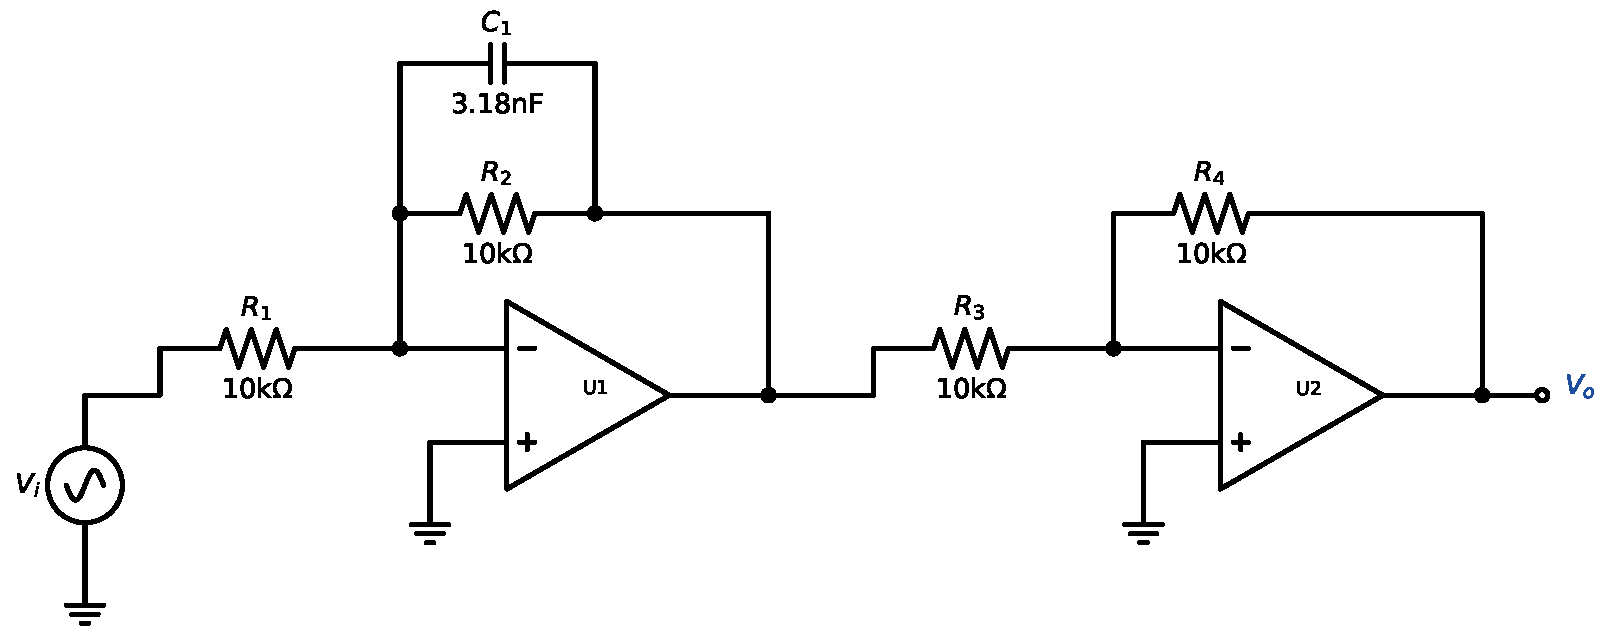
\includegraphics[width=\linewidth,height=5.5cm,keepaspectratio]{p03_design}\end{center}
Check: the stage gains multiply to $(-1)^{2}\cdot1\cdot(\text{factors}) = H(s)$; an independent nodal solve of this circuit reproduces $H(s)$ at every frequency. (Standard-value resistors and capacitors would move the corners slightly.)

The input is $V_i(t) = 1\cos\left(2\pi\cdot 10000\,t\right)$, so $\omega_{in} = 2\pi\cdot 10000 = 62800$\,rad/s. Put $s=j\omega_{in}$ in each factor (tool T5): magnitudes multiply, angles add.
{\small Rules: $\left|\frac{s}{s+p}\right| = \frac{\omega}{\sqrt{\omega^2+p^2}}$, $\angle = \frac{\pi}{2}-\tan^{-1}\frac{\omega}{p}$;\quad $\left|\frac{1}{1+s/p}\right| = \frac{1}{\sqrt{1+(\omega/p)^2}}$, $\angle = -\tan^{-1}\frac{\omega}{p}$;\quad $\left|1+\frac{s}{z}\right| = \sqrt{1+(\omega/z)^2}$, $\angle = \tan^{-1}\frac{\omega}{z}$;\quad a negative $K$ adds $-\pi$.}
\begin{center}\renewcommand{\arraystretch}{1.35}
\begin{tabular}{ccc}
\toprule
factor & magnitude & angle (rad) \\
\midrule
$1$ & $1$ & $0$ \\
$\rule[-1.7em]{0pt}{4em}\dfrac{1}{1+\dfrac{s}{2\pi\cdot 5\mathrm{k}}}$ & $0.4472$ & $-1.11$ \\
\textbf{total} & $\mathbf{0.4472}$ (product) & $\mathbf{-1.11}$ (sum) \\
\bottomrule
\end{tabular}\end{center}

\begin{align*}
|H(j\omega_{in})| &= 0.447, \qquad \angle H(j\omega_{in}) = -1.11\ \mathrm{rad} \\
v_{o,ac}(t) &= 0.447\times 1\,\cos\left(2\pi\cdot 10000\,t - 1.11\right) = 0.447\,\cos\left(2\pi\cdot 10000\,t - 1.11\right)
\end{align*}

\[
\boxed{V_o(t) = 0.447\,\cos\left(2\pi\cdot 10000\,t - 1.11\right)\ \mathrm{V}}
\]

\begin{ansbox}
$H(s) = 1\,\dfrac{1}{1+\dfrac{s}{2\pi\cdot 5\mathrm{k}}}$\\[4pt]
U1: R1 = 10k$\Omega$, R2 = 10k$\Omega$, C1 = 3.18nF\\
U2: R3 = 10k$\Omega$, R4 = 10k$\Omega$\\[4pt]
$V_o(t) = 0.447\,\cos\left(2\pi\cdot 10000\,t - 1.11\right)\ \mathrm{V}$
\end{ansbox}

\newpage
\subsection*{Solution 2C.4 \hfill Easy}
\begin{center}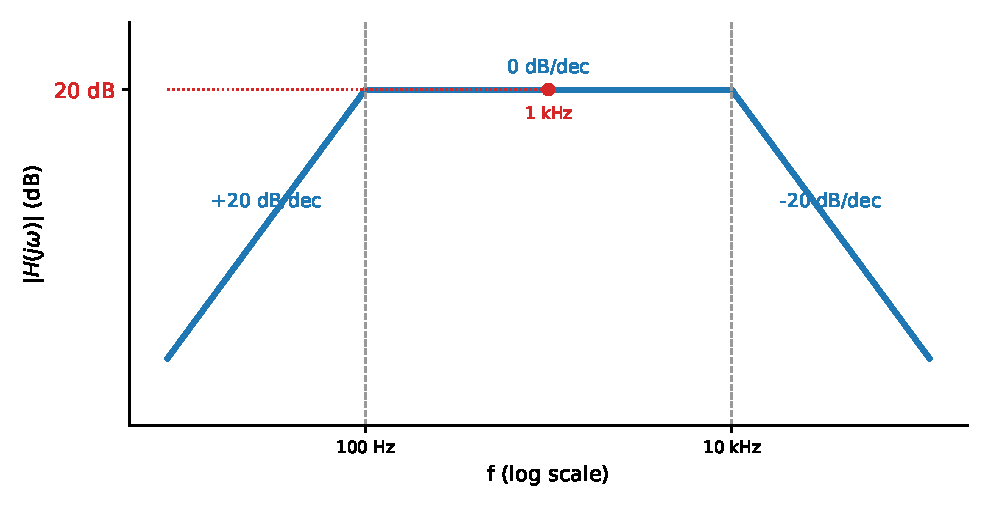
\includegraphics[width=\linewidth,height=5cm,keepaspectratio]{p04_plot}\end{center}
\solstep{1}{Read the corners and slopes}Go left to right along the plot and write down the slope of every straight segment. At each corner frequency the slope changes by a multiple of 20\,dB/dec: every $-20$ is one pole, every $+20$ is one zero (tool T6 read backwards).\begin{center}\renewcommand{\arraystretch}{1.35}
\begin{tabular}{ccccl}
\toprule
corner $f_c$ & slope before & slope after & change & meaning \\
\midrule
100 Hz & $+20$ & $0$ & $-20$ & one pole at $f_c$ \\
10 kHz & $0$ & $-20$ & $-20$ & one pole at $f_c$ \\
\bottomrule
\end{tabular}\end{center}

\solstep{2}{Starting slope $\Rightarrow$ factors of $s$}The plot starts with a slope of $+20$\,dB/dec, i.e. $|H|\propto\omega^1$ at low frequency: the numerator contains $s$. As in class, pair each $s$ with one of the \emph{lowest} poles (100 Hz) as $\frac{s}{s+p}$: such a factor rises at $+20$\,dB/dec below $p$ and is $\approx1$ (0\,dB) above it. The remaining poles are written $\frac{1}{1+s/p}$ and the zeros $\left(1+\frac{s}{z}\right)$. Every corner is an angular frequency $\omega_c=2\pi f_c$.
\solstep{3}{Assemble $H(s)$}Put one factor per pole/zero in front of an unknown constant $K$:\[
H(s) = K\,\dfrac{s}{s+2\pi\cdot 100}\,\dfrac{1}{1+\dfrac{s}{2\pi\cdot 10\mathrm{k}}}
\]

\solstep{4}{Find $K$ from the marked level}The plot marks the level $20$\,dB at $f=$\,1 kHz. On the straight-line plot every factor is either exactly 0\,dB (where it is $\approx1$) or a $\pm20$\,dB/dec line, so evaluate the \emph{asymptote} of each factor at that frequency (the level of a line with slope $\pm20$\,dB/dec is $\pm20\log_{10}(f/f_c)$):\begin{center}\renewcommand{\arraystretch}{1.35}
\begin{tabular}{cccc}
\toprule
factor & $f_c$ & at $f=$\,1 kHz & asymptote (dB) \\
\midrule
$\rule[-1.1em]{0pt}{2.8em}\dfrac{s}{s+2\pi\cdot 100}$ & 100 Hz & $f>f_c$: $\approx 1$ & $0$ \\
$\rule[-1.7em]{0pt}{4em}\dfrac{1}{1+\dfrac{s}{2\pi\cdot 10\mathrm{k}}}$ & 10 kHz & $f<f_c$: $\approx 1$ & $0$ \\
\textbf{sum} &  &  & $\mathbf{0}$ \\
\bottomrule
\end{tabular}\end{center}
The dB values of the factors \emph{add} (magnitudes multiply), so\[
20\log_{10}K = 20 - (0) = 20\ \mathrm{dB}\quad\Rightarrow\quad K = 10^{20/20} = 10
\]

So\[
\boxed{H(s) = 10\,\dfrac{s}{s+2\pi\cdot 100}\,\dfrac{1}{1+\dfrac{s}{2\pi\cdot 10\mathrm{k}}}}
\]


\solstep{5}{Split $H(s)$ into op-amp stages}Every inverting stage of the form $-\frac{Z_f}{Z_{in}}$ with $Z_{in}$, $Z_f$ made of one R and at most one C realizes \emph{one} pole, optionally with one zero or one $s$ (tool T2). Pair each zero with a low-pass pole (pole-zero stage), each $\frac{s}{s+p}$ with a remaining low-pass pole (band-pass stage), and give every leftover factor its own stage. Put all of $|K|$ into the first stage. Each stage inverts, so with an odd number of stages add a unity-gain inverter to make $K>0$.\begin{center}\renewcommand{\arraystretch}{1.35}
\begin{tabular}{cccl}
\toprule
stage & gain $\frac{R_2}{R_1}$ & factor(s) realized & block \\
\midrule
U1 & $10$ & $\rule[-1.4em]{0pt}{3.4em}\dfrac{s}{s+2\pi\cdot 100}\cdot\dfrac{1}{1+\frac{s}{2\pi\cdot 10\mathrm{k}}}$ & band-pass: $Z_{in}=R+\frac{1}{sC}$, $Z_f=R\parallel C$ \\
U2 & $1$ & $\rule[-1.4em]{0pt}{3.4em}1$ & unity inverter (fixes the sign) \\
\bottomrule
\end{tabular}\end{center}

\solstep{6}{Component values}Use $R_1 = 10\,\mathrm{k}\Omega$ at the input of every stage (any convenient value works; it only scales the other parts). The corner of a factor $1+s/\omega_c$ is matched by $RC = 1/\omega_c$ (corners in rad/s).\begin{enumerate}[leftmargin=*,itemsep=2pt]
\item U1: choose $R_{1} = 10\,\mathrm{k}\Omega$, then match the stage formula $-\frac{R_{2}}{R_{1}}\cdot\frac{s}{s+1/(R_{1}C_{1})}\cdot\frac{1}{1+sR_{2}C_{2}}$ to the factors:\[
C_{1} = \frac{1}{628\,R_{1}} = 159\,\mathrm{n}\mathrm{F},\qquad R_{2} = 10\,R_{1} = 100\,\mathrm{k}\Omega,\qquad C_{2} = \frac{1}{62800\,R_{2}} = 159\,\mathrm{p}\mathrm{F}
\]

\item U2: $R_{3} = R_{4} = 10\,\mathrm{k}\Omega$ (gain $-1$).
\end{enumerate}

\solstep{7}{Check and steady-state output}The designed circuit:\begin{center}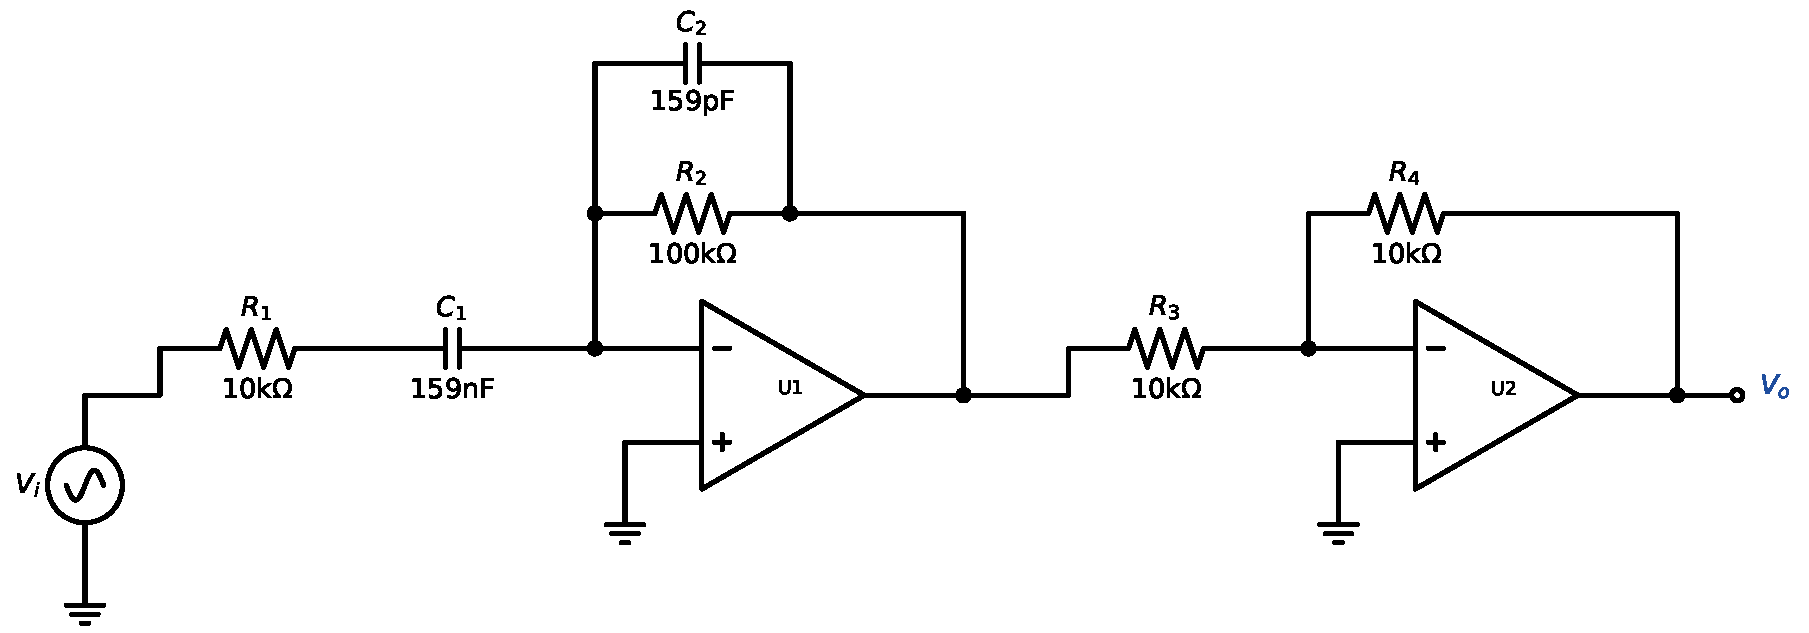
\includegraphics[width=\linewidth,height=5.5cm,keepaspectratio]{p04_design}\end{center}
Check: the stage gains multiply to $(-1)^{2}\cdot10\cdot(\text{factors}) = H(s)$; an independent nodal solve of this circuit reproduces $H(s)$ at every frequency. (Standard-value resistors and capacitors would move the corners slightly.)

The input is $V_i(t) = 0.05\sin\left(2\pi\cdot 300\,t\right)$, so $\omega_{in} = 2\pi\cdot 300 = 1880$\,rad/s. Put $s=j\omega_{in}$ in each factor (tool T5): magnitudes multiply, angles add.
{\small Rules: $\left|\frac{s}{s+p}\right| = \frac{\omega}{\sqrt{\omega^2+p^2}}$, $\angle = \frac{\pi}{2}-\tan^{-1}\frac{\omega}{p}$;\quad $\left|\frac{1}{1+s/p}\right| = \frac{1}{\sqrt{1+(\omega/p)^2}}$, $\angle = -\tan^{-1}\frac{\omega}{p}$;\quad $\left|1+\frac{s}{z}\right| = \sqrt{1+(\omega/z)^2}$, $\angle = \tan^{-1}\frac{\omega}{z}$;\quad a negative $K$ adds $-\pi$.}
\begin{center}\renewcommand{\arraystretch}{1.35}
\begin{tabular}{ccc}
\toprule
factor & magnitude & angle (rad) \\
\midrule
$10$ & $10$ & $0$ \\
$\rule[-1.1em]{0pt}{2.8em}\dfrac{s}{s+2\pi\cdot 100}$ & $0.9487$ & $0.322$ \\
$\rule[-1.7em]{0pt}{4em}\dfrac{1}{1+\dfrac{s}{2\pi\cdot 10\mathrm{k}}}$ & $0.9996$ & $-0.03$ \\
\textbf{total} & $\mathbf{9.483}$ (product) & $\mathbf{0.292}$ (sum) \\
\bottomrule
\end{tabular}\end{center}

\begin{align*}
|H(j\omega_{in})| &= 9.48, \qquad \angle H(j\omega_{in}) = 0.292\ \mathrm{rad} \\
v_{o,ac}(t) &= 9.48\times 0.05\,\sin\left(2\pi\cdot 300\,t + 0.292\right) = 0.474\,\sin\left(2\pi\cdot 300\,t + 0.292\right)
\end{align*}

\[
\boxed{V_o(t) = 0.474\,\sin\left(2\pi\cdot 300\,t + 0.292\right)\ \mathrm{V}}
\]

\begin{ansbox}
$H(s) = 10\,\dfrac{s}{s+2\pi\cdot 100}\,\dfrac{1}{1+\dfrac{s}{2\pi\cdot 10\mathrm{k}}}$\\[4pt]
U1: R1 = 10k$\Omega$, C1 = 159nF, R2 = 100k$\Omega$, C2 = 159pF\\
U2: R3 = 10k$\Omega$, R4 = 10k$\Omega$\\[4pt]
$V_o(t) = 0.474\,\sin\left(2\pi\cdot 300\,t + 0.292\right)\ \mathrm{V}$
\end{ansbox}

\newpage
\subsection*{Solution 2C.5 \hfill Easy}
\begin{center}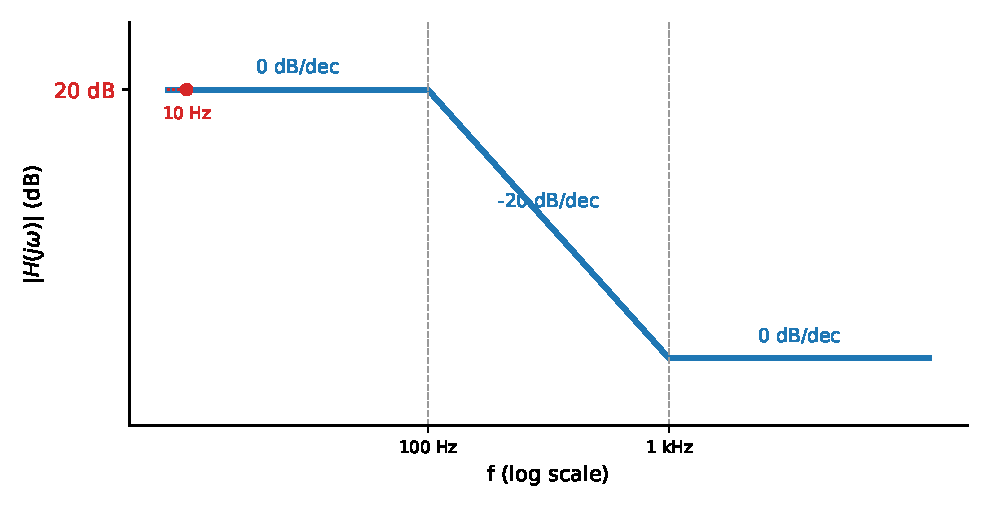
\includegraphics[width=\linewidth,height=5cm,keepaspectratio]{p05_plot}\end{center}
\solstep{1}{Read the corners and slopes}Go left to right along the plot and write down the slope of every straight segment. At each corner frequency the slope changes by a multiple of 20\,dB/dec: every $-20$ is one pole, every $+20$ is one zero (tool T6 read backwards).\begin{center}\renewcommand{\arraystretch}{1.35}
\begin{tabular}{ccccl}
\toprule
corner $f_c$ & slope before & slope after & change & meaning \\
\midrule
100 Hz & $0$ & $-20$ & $-20$ & one pole at $f_c$ \\
1 kHz & $-20$ & $0$ & $+20$ & one zero at $f_c$ \\
\bottomrule
\end{tabular}\end{center}

\solstep{2}{Starting slope $\Rightarrow$ factors of $s$}The plot starts \emph{flat} (0\,dB/dec), so there is no factor $s$ in the numerator: every pole is written as $\frac{1}{1+s/p}$ and every zero as $\left(1+\frac{s}{z}\right)$, which are all $\approx1$ (0\,dB) at low frequency. Every corner is an angular frequency $\omega_c=2\pi f_c$.
\solstep{3}{Assemble $H(s)$}Put one factor per pole/zero in front of an unknown constant $K$:\[
H(s) = K\,\dfrac{1}{1+\dfrac{s}{2\pi\cdot 100}}\,\left(1+\dfrac{s}{2\pi\cdot 1\mathrm{k}}\right)
\]

\solstep{4}{Find $K$ from the marked level}The plot marks the level $20$\,dB at $f=$\,10 Hz. On the straight-line plot every factor is either exactly 0\,dB (where it is $\approx1$) or a $\pm20$\,dB/dec line, so evaluate the \emph{asymptote} of each factor at that frequency (the level of a line with slope $\pm20$\,dB/dec is $\pm20\log_{10}(f/f_c)$):\begin{center}\renewcommand{\arraystretch}{1.35}
\begin{tabular}{cccc}
\toprule
factor & $f_c$ & at $f=$\,10 Hz & asymptote (dB) \\
\midrule
$\rule[-1.7em]{0pt}{4em}\dfrac{1}{1+\dfrac{s}{2\pi\cdot 100}}$ & 100 Hz & $f<f_c$: $\approx 1$ & $0$ \\
$\rule[-1.1em]{0pt}{2.8em}\left(1+\dfrac{s}{2\pi\cdot 1\mathrm{k}}\right)$ & 1 kHz & $f<f_c$: $\approx 1$ & $0$ \\
\textbf{sum} &  &  & $\mathbf{0}$ \\
\bottomrule
\end{tabular}\end{center}
The dB values of the factors \emph{add} (magnitudes multiply), so\[
20\log_{10}K = 20 - (0) = 20\ \mathrm{dB}\quad\Rightarrow\quad K = 10^{20/20} = 10
\]

So\[
\boxed{H(s) = 10\,\dfrac{1}{1+\dfrac{s}{2\pi\cdot 100}}\,\left(1+\dfrac{s}{2\pi\cdot 1\mathrm{k}}\right)}
\]


\solstep{5}{Split $H(s)$ into op-amp stages}Every inverting stage of the form $-\frac{Z_f}{Z_{in}}$ with $Z_{in}$, $Z_f$ made of one R and at most one C realizes \emph{one} pole, optionally with one zero or one $s$ (tool T2). Pair each zero with a low-pass pole (pole-zero stage), each $\frac{s}{s+p}$ with a remaining low-pass pole (band-pass stage), and give every leftover factor its own stage. Put all of $|K|$ into the first stage. Each stage inverts, so with an odd number of stages add a unity-gain inverter to make $K>0$.\begin{center}\renewcommand{\arraystretch}{1.35}
\begin{tabular}{cccl}
\toprule
stage & gain $\frac{R_2}{R_1}$ & factor(s) realized & block \\
\midrule
U1 & $10$ & $\rule[-1.4em]{0pt}{3.4em}\dfrac{1+\frac{s}{2\pi\cdot 1\mathrm{k}}}{1+\frac{s}{2\pi\cdot 100}}$ & pole-zero: $Z_{in}=R\parallel C$, $Z_f = R\parallel C$ \\
U2 & $1$ & $\rule[-1.4em]{0pt}{3.4em}1$ & unity inverter (fixes the sign) \\
\bottomrule
\end{tabular}\end{center}

\solstep{6}{Component values}Use $R_1 = 10\,\mathrm{k}\Omega$ at the input of every stage (any convenient value works; it only scales the other parts). The corner of a factor $1+s/\omega_c$ is matched by $RC = 1/\omega_c$ (corners in rad/s).\begin{enumerate}[leftmargin=*,itemsep=2pt]
\item U1: choose $R_{1} = 10\,\mathrm{k}\Omega$, then match the stage formula $-\frac{R_{2}}{R_{1}}\cdot\frac{1+sR_{1}C_{1}}{1+sR_{2}C_{2}}$ to the factors:\[
R_{2} = 10\,R_{1} = 100\,\mathrm{k}\Omega,\qquad C_{1} = \frac{1}{6280\,R_{1}} = 15.9\,\mathrm{n}\mathrm{F},\qquad C_{2} = \frac{1}{628\,R_{2}} = 15.9\,\mathrm{n}\mathrm{F}
\]

\item U2: $R_{3} = R_{4} = 10\,\mathrm{k}\Omega$ (gain $-1$).
\end{enumerate}

\solstep{7}{Check and steady-state output}The designed circuit:\begin{center}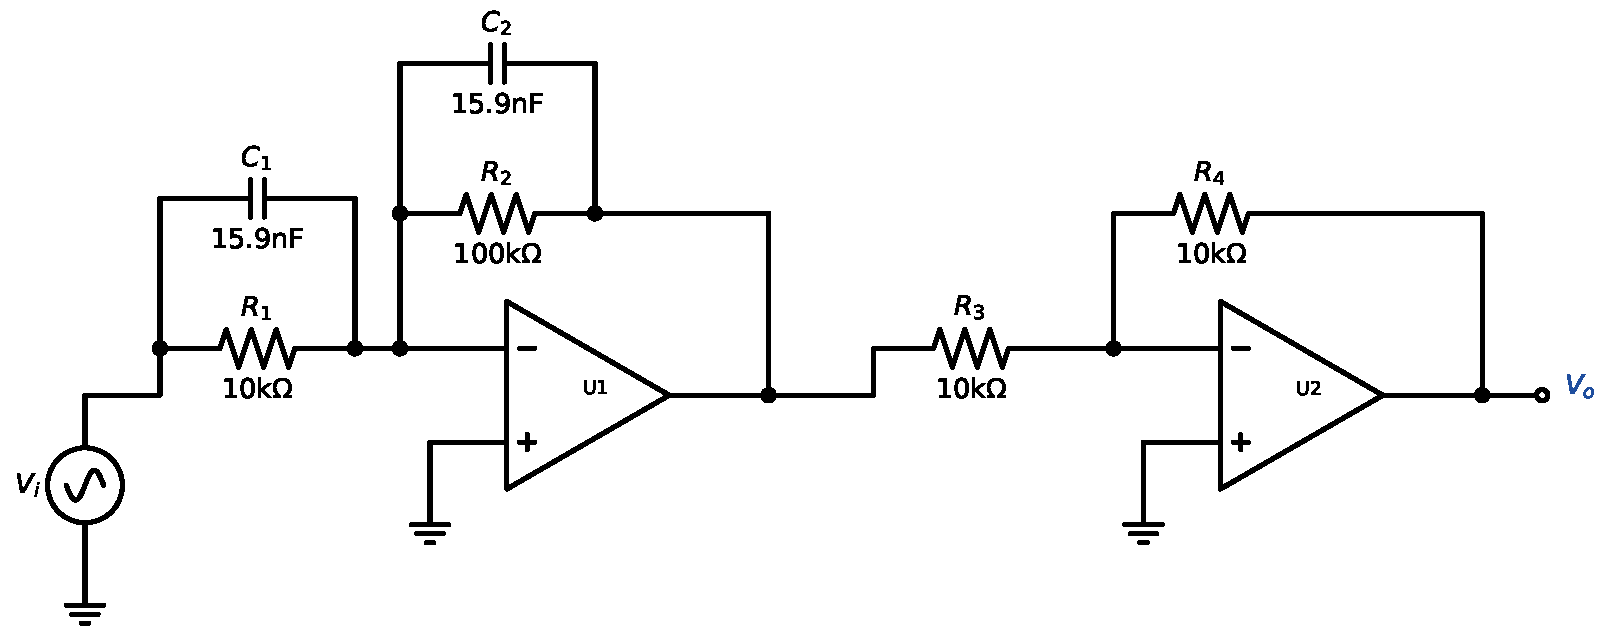
\includegraphics[width=\linewidth,height=5.5cm,keepaspectratio]{p05_design}\end{center}
Check: the stage gains multiply to $(-1)^{2}\cdot10\cdot(\text{factors}) = H(s)$; an independent nodal solve of this circuit reproduces $H(s)$ at every frequency. (Standard-value resistors and capacitors would move the corners slightly.)

The input is $V_i(t) = 0.1\sin\left(2\pi\cdot 500\,t\right)$, so $\omega_{in} = 2\pi\cdot 500 = 3140$\,rad/s. Put $s=j\omega_{in}$ in each factor (tool T5): magnitudes multiply, angles add.
{\small Rules: $\left|\frac{s}{s+p}\right| = \frac{\omega}{\sqrt{\omega^2+p^2}}$, $\angle = \frac{\pi}{2}-\tan^{-1}\frac{\omega}{p}$;\quad $\left|\frac{1}{1+s/p}\right| = \frac{1}{\sqrt{1+(\omega/p)^2}}$, $\angle = -\tan^{-1}\frac{\omega}{p}$;\quad $\left|1+\frac{s}{z}\right| = \sqrt{1+(\omega/z)^2}$, $\angle = \tan^{-1}\frac{\omega}{z}$;\quad a negative $K$ adds $-\pi$.}
\begin{center}\renewcommand{\arraystretch}{1.35}
\begin{tabular}{ccc}
\toprule
factor & magnitude & angle (rad) \\
\midrule
$10$ & $10$ & $0$ \\
$\rule[-1.7em]{0pt}{4em}\dfrac{1}{1+\dfrac{s}{2\pi\cdot 100}}$ & $0.1961$ & $-1.37$ \\
$\rule[-1.1em]{0pt}{2.8em}\left(1+\dfrac{s}{2\pi\cdot 1\mathrm{k}}\right)$ & $1.118$ & $0.464$ \\
\textbf{total} & $\mathbf{2.193}$ (product) & $\mathbf{-0.91}$ (sum) \\
\bottomrule
\end{tabular}\end{center}

\begin{align*}
|H(j\omega_{in})| &= 2.19, \qquad \angle H(j\omega_{in}) = -0.91\ \mathrm{rad} \\
v_{o,ac}(t) &= 2.19\times 0.1\,\sin\left(2\pi\cdot 500\,t - 0.91\right) = 0.219\,\sin\left(2\pi\cdot 500\,t - 0.91\right)
\end{align*}

\[
\boxed{V_o(t) = 0.219\,\sin\left(2\pi\cdot 500\,t - 0.91\right)\ \mathrm{V}}
\]

\begin{ansbox}
$H(s) = 10\,\dfrac{1}{1+\dfrac{s}{2\pi\cdot 100}}\,\left(1+\dfrac{s}{2\pi\cdot 1\mathrm{k}}\right)$\\[4pt]
U1: R1 = 10k$\Omega$, C1 = 15.9nF, R2 = 100k$\Omega$, C2 = 15.9nF\\
U2: R3 = 10k$\Omega$, R4 = 10k$\Omega$\\[4pt]
$V_o(t) = 0.219\,\sin\left(2\pi\cdot 500\,t - 0.91\right)\ \mathrm{V}$
\end{ansbox}

\newpage
\subsection*{Solution 2C.6 \hfill Easy}
\begin{center}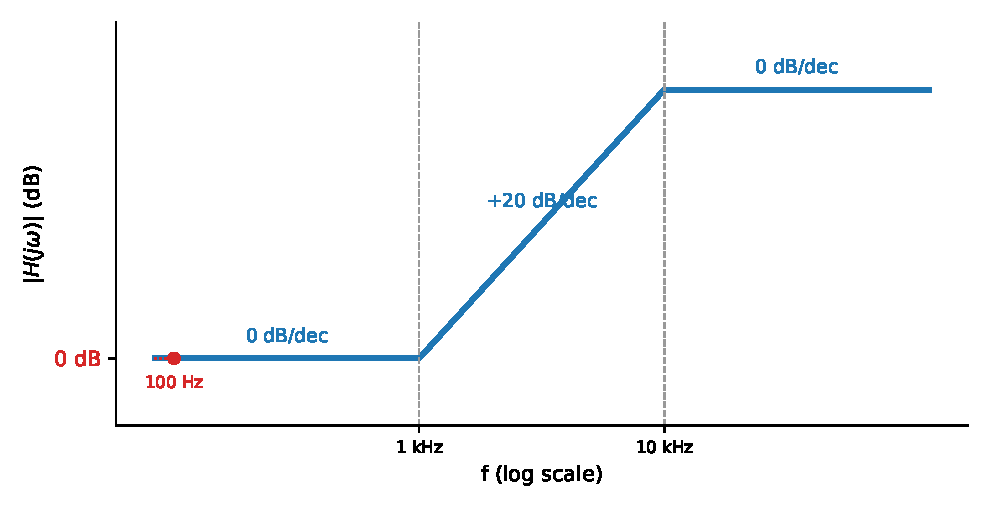
\includegraphics[width=\linewidth,height=5cm,keepaspectratio]{p06_plot}\end{center}
\solstep{1}{Read the corners and slopes}Go left to right along the plot and write down the slope of every straight segment. At each corner frequency the slope changes by a multiple of 20\,dB/dec: every $-20$ is one pole, every $+20$ is one zero (tool T6 read backwards).\begin{center}\renewcommand{\arraystretch}{1.35}
\begin{tabular}{ccccl}
\toprule
corner $f_c$ & slope before & slope after & change & meaning \\
\midrule
1 kHz & $0$ & $+20$ & $+20$ & one zero at $f_c$ \\
10 kHz & $+20$ & $0$ & $-20$ & one pole at $f_c$ \\
\bottomrule
\end{tabular}\end{center}

\solstep{2}{Starting slope $\Rightarrow$ factors of $s$}The plot starts \emph{flat} (0\,dB/dec), so there is no factor $s$ in the numerator: every pole is written as $\frac{1}{1+s/p}$ and every zero as $\left(1+\frac{s}{z}\right)$, which are all $\approx1$ (0\,dB) at low frequency. Every corner is an angular frequency $\omega_c=2\pi f_c$.
\solstep{3}{Assemble $H(s)$}Put one factor per pole/zero in front of an unknown constant $K$:\[
H(s) = K\,\left(1+\dfrac{s}{2\pi\cdot 1\mathrm{k}}\right)\,\dfrac{1}{1+\dfrac{s}{2\pi\cdot 10\mathrm{k}}}
\]

\solstep{4}{Find $K$ from the marked level}The plot marks the level $0$\,dB at $f=$\,100 Hz. On the straight-line plot every factor is either exactly 0\,dB (where it is $\approx1$) or a $\pm20$\,dB/dec line, so evaluate the \emph{asymptote} of each factor at that frequency (the level of a line with slope $\pm20$\,dB/dec is $\pm20\log_{10}(f/f_c)$):\begin{center}\renewcommand{\arraystretch}{1.35}
\begin{tabular}{cccc}
\toprule
factor & $f_c$ & at $f=$\,100 Hz & asymptote (dB) \\
\midrule
$\rule[-1.1em]{0pt}{2.8em}\left(1+\dfrac{s}{2\pi\cdot 1\mathrm{k}}\right)$ & 1 kHz & $f<f_c$: $\approx 1$ & $0$ \\
$\rule[-1.7em]{0pt}{4em}\dfrac{1}{1+\dfrac{s}{2\pi\cdot 10\mathrm{k}}}$ & 10 kHz & $f<f_c$: $\approx 1$ & $0$ \\
\textbf{sum} &  &  & $\mathbf{0}$ \\
\bottomrule
\end{tabular}\end{center}
The dB values of the factors \emph{add} (magnitudes multiply), so\[
20\log_{10}K = 0 - (0) = 0\ \mathrm{dB}\quad\Rightarrow\quad K = 10^{0/20} = 1
\]

So\[
\boxed{H(s) = 1\,\left(1+\dfrac{s}{2\pi\cdot 1\mathrm{k}}\right)\,\dfrac{1}{1+\dfrac{s}{2\pi\cdot 10\mathrm{k}}}}
\]


\solstep{5}{Split $H(s)$ into op-amp stages}Every inverting stage of the form $-\frac{Z_f}{Z_{in}}$ with $Z_{in}$, $Z_f$ made of one R and at most one C realizes \emph{one} pole, optionally with one zero or one $s$ (tool T2). Pair each zero with a low-pass pole (pole-zero stage), each $\frac{s}{s+p}$ with a remaining low-pass pole (band-pass stage), and give every leftover factor its own stage. Put all of $|K|$ into the first stage. Each stage inverts, so with an odd number of stages add a unity-gain inverter to make $K>0$.\begin{center}\renewcommand{\arraystretch}{1.35}
\begin{tabular}{cccl}
\toprule
stage & gain $\frac{R_2}{R_1}$ & factor(s) realized & block \\
\midrule
U1 & $1$ & $\rule[-1.4em]{0pt}{3.4em}\dfrac{1+\frac{s}{2\pi\cdot 1\mathrm{k}}}{1+\frac{s}{2\pi\cdot 10\mathrm{k}}}$ & pole-zero: $Z_{in}=R\parallel C$, $Z_f = R\parallel C$ \\
U2 & $1$ & $\rule[-1.4em]{0pt}{3.4em}1$ & unity inverter (fixes the sign) \\
\bottomrule
\end{tabular}\end{center}

\solstep{6}{Component values}Use $R_1 = 10\,\mathrm{k}\Omega$ at the input of every stage (any convenient value works; it only scales the other parts). The corner of a factor $1+s/\omega_c$ is matched by $RC = 1/\omega_c$ (corners in rad/s).\begin{enumerate}[leftmargin=*,itemsep=2pt]
\item U1: choose $R_{1} = 10\,\mathrm{k}\Omega$, then match the stage formula $-\frac{R_{2}}{R_{1}}\cdot\frac{1+sR_{1}C_{1}}{1+sR_{2}C_{2}}$ to the factors:\[
R_{2} = 1\,R_{1} = 10\,\mathrm{k}\Omega,\qquad C_{1} = \frac{1}{6280\,R_{1}} = 15.9\,\mathrm{n}\mathrm{F},\qquad C_{2} = \frac{1}{62800\,R_{2}} = 1.59\,\mathrm{n}\mathrm{F}
\]

\item U2: $R_{3} = R_{4} = 10\,\mathrm{k}\Omega$ (gain $-1$).
\end{enumerate}

\solstep{7}{Check and steady-state output}The designed circuit:\begin{center}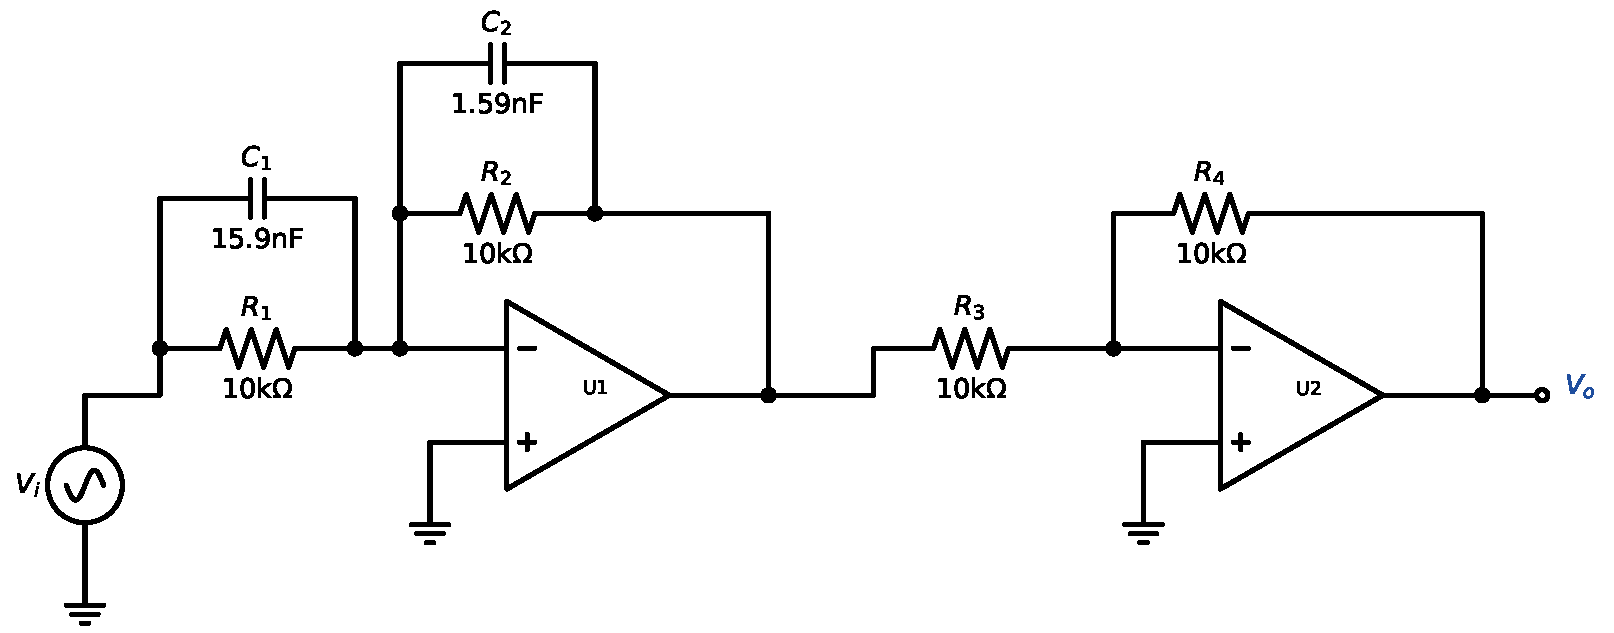
\includegraphics[width=\linewidth,height=5.5cm,keepaspectratio]{p06_design}\end{center}
Check: the stage gains multiply to $(-1)^{2}\cdot1\cdot(\text{factors}) = H(s)$; an independent nodal solve of this circuit reproduces $H(s)$ at every frequency. (Standard-value resistors and capacitors would move the corners slightly.)

The input is $V_i(t) = 0.5\sin\left(2\pi\cdot 3000\,t\right)$, so $\omega_{in} = 2\pi\cdot 3000 = 18800$\,rad/s. Put $s=j\omega_{in}$ in each factor (tool T5): magnitudes multiply, angles add.
{\small Rules: $\left|\frac{s}{s+p}\right| = \frac{\omega}{\sqrt{\omega^2+p^2}}$, $\angle = \frac{\pi}{2}-\tan^{-1}\frac{\omega}{p}$;\quad $\left|\frac{1}{1+s/p}\right| = \frac{1}{\sqrt{1+(\omega/p)^2}}$, $\angle = -\tan^{-1}\frac{\omega}{p}$;\quad $\left|1+\frac{s}{z}\right| = \sqrt{1+(\omega/z)^2}$, $\angle = \tan^{-1}\frac{\omega}{z}$;\quad a negative $K$ adds $-\pi$.}
\begin{center}\renewcommand{\arraystretch}{1.35}
\begin{tabular}{ccc}
\toprule
factor & magnitude & angle (rad) \\
\midrule
$1$ & $1$ & $0$ \\
$\rule[-1.1em]{0pt}{2.8em}\left(1+\dfrac{s}{2\pi\cdot 1\mathrm{k}}\right)$ & $3.162$ & $1.25$ \\
$\rule[-1.7em]{0pt}{4em}\dfrac{1}{1+\dfrac{s}{2\pi\cdot 10\mathrm{k}}}$ & $0.9578$ & $-0.291$ \\
\textbf{total} & $\mathbf{3.029}$ (product) & $\mathbf{0.958}$ (sum) \\
\bottomrule
\end{tabular}\end{center}

\begin{align*}
|H(j\omega_{in})| &= 3.03, \qquad \angle H(j\omega_{in}) = 0.958\ \mathrm{rad} \\
v_{o,ac}(t) &= 3.03\times 0.5\,\sin\left(2\pi\cdot 3000\,t + 0.958\right) = 1.51\,\sin\left(2\pi\cdot 3000\,t + 0.958\right)
\end{align*}

\[
\boxed{V_o(t) = 1.51\,\sin\left(2\pi\cdot 3000\,t + 0.958\right)\ \mathrm{V}}
\]

\begin{ansbox}
$H(s) = 1\,\left(1+\dfrac{s}{2\pi\cdot 1\mathrm{k}}\right)\,\dfrac{1}{1+\dfrac{s}{2\pi\cdot 10\mathrm{k}}}$\\[4pt]
U1: R1 = 10k$\Omega$, C1 = 15.9nF, R2 = 10k$\Omega$, C2 = 1.59nF\\
U2: R3 = 10k$\Omega$, R4 = 10k$\Omega$\\[4pt]
$V_o(t) = 1.51\,\sin\left(2\pi\cdot 3000\,t + 0.958\right)\ \mathrm{V}$
\end{ansbox}

\newpage
\subsection*{Solution 2C.7 \hfill Medium}
\begin{center}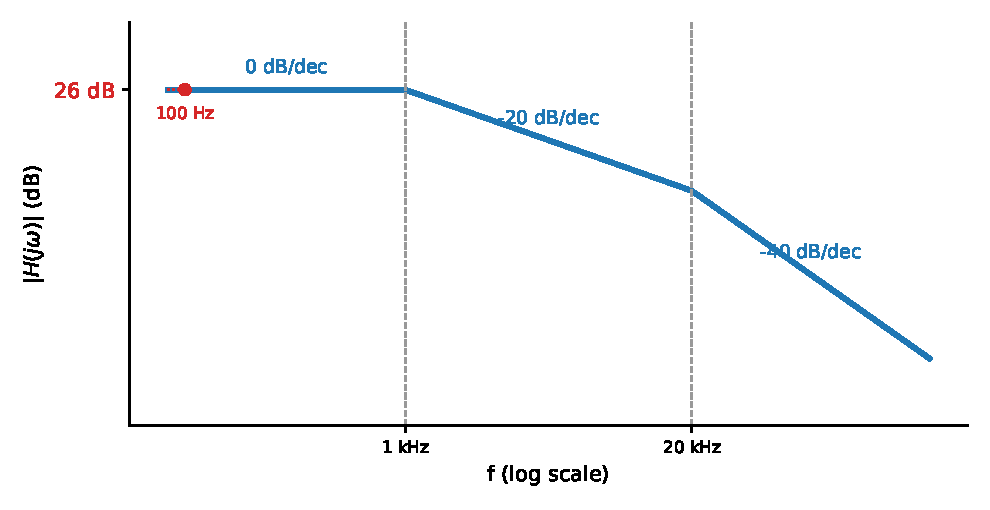
\includegraphics[width=\linewidth,height=5cm,keepaspectratio]{p07_plot}\end{center}
\solstep{1}{Read the corners and slopes}Go left to right along the plot and write down the slope of every straight segment. At each corner frequency the slope changes by a multiple of 20\,dB/dec: every $-20$ is one pole, every $+20$ is one zero (tool T6 read backwards).\begin{center}\renewcommand{\arraystretch}{1.35}
\begin{tabular}{ccccl}
\toprule
corner $f_c$ & slope before & slope after & change & meaning \\
\midrule
1 kHz & $0$ & $-20$ & $-20$ & one pole at $f_c$ \\
20 kHz & $-20$ & $-40$ & $-20$ & one pole at $f_c$ \\
\bottomrule
\end{tabular}\end{center}

\solstep{2}{Starting slope $\Rightarrow$ factors of $s$}The plot starts \emph{flat} (0\,dB/dec), so there is no factor $s$ in the numerator: every pole is written as $\frac{1}{1+s/p}$ and every zero as $\left(1+\frac{s}{z}\right)$, which are all $\approx1$ (0\,dB) at low frequency. Every corner is an angular frequency $\omega_c=2\pi f_c$.
\solstep{3}{Assemble $H(s)$}Put one factor per pole/zero in front of an unknown constant $K$:\[
H(s) = K\,\dfrac{1}{1+\dfrac{s}{2\pi\cdot 1\mathrm{k}}}\,\dfrac{1}{1+\dfrac{s}{2\pi\cdot 20\mathrm{k}}}
\]

\solstep{4}{Find $K$ from the marked level}The plot marks the level $26$\,dB at $f=$\,100 Hz. On the straight-line plot every factor is either exactly 0\,dB (where it is $\approx1$) or a $\pm20$\,dB/dec line, so evaluate the \emph{asymptote} of each factor at that frequency (the level of a line with slope $\pm20$\,dB/dec is $\pm20\log_{10}(f/f_c)$):\begin{center}\renewcommand{\arraystretch}{1.35}
\begin{tabular}{cccc}
\toprule
factor & $f_c$ & at $f=$\,100 Hz & asymptote (dB) \\
\midrule
$\rule[-1.7em]{0pt}{4em}\dfrac{1}{1+\dfrac{s}{2\pi\cdot 1\mathrm{k}}}$ & 1 kHz & $f<f_c$: $\approx 1$ & $0$ \\
$\rule[-1.7em]{0pt}{4em}\dfrac{1}{1+\dfrac{s}{2\pi\cdot 20\mathrm{k}}}$ & 20 kHz & $f<f_c$: $\approx 1$ & $0$ \\
\textbf{sum} &  &  & $\mathbf{0}$ \\
\bottomrule
\end{tabular}\end{center}
The dB values of the factors \emph{add} (magnitudes multiply), so\[
20\log_{10}K = 26 - (0) = 26\ \mathrm{dB}\quad\Rightarrow\quad K = 10^{26/20} = 20
\]

So\[
\boxed{H(s) = 20\,\dfrac{1}{1+\dfrac{s}{2\pi\cdot 1\mathrm{k}}}\,\dfrac{1}{1+\dfrac{s}{2\pi\cdot 20\mathrm{k}}}}
\]


\solstep{5}{Split $H(s)$ into op-amp stages}Every inverting stage of the form $-\frac{Z_f}{Z_{in}}$ with $Z_{in}$, $Z_f$ made of one R and at most one C realizes \emph{one} pole, optionally with one zero or one $s$ (tool T2). Pair each zero with a low-pass pole (pole-zero stage), each $\frac{s}{s+p}$ with a remaining low-pass pole (band-pass stage), and give every leftover factor its own stage. Put all of $|K|$ into the first stage. Each stage inverts, so with an odd number of stages add a unity-gain inverter to make $K>0$.\begin{center}\renewcommand{\arraystretch}{1.35}
\begin{tabular}{cccl}
\toprule
stage & gain $\frac{R_2}{R_1}$ & factor(s) realized & block \\
\midrule
U1 & $19.95$ & $\rule[-1.4em]{0pt}{3.4em}\dfrac{1}{1+\frac{s}{2\pi\cdot 1\mathrm{k}}}$ & low-pass: $Z_{in}=R$, $Z_f=R\parallel C$ \\
U2 & $1$ & $\rule[-1.4em]{0pt}{3.4em}\dfrac{1}{1+\frac{s}{2\pi\cdot 20\mathrm{k}}}$ & low-pass: $Z_{in}=R$, $Z_f=R\parallel C$ \\
\bottomrule
\end{tabular}\end{center}

\solstep{6}{Component values}Use $R_1 = 10\,\mathrm{k}\Omega$ at the input of every stage (any convenient value works; it only scales the other parts). The corner of a factor $1+s/\omega_c$ is matched by $RC = 1/\omega_c$ (corners in rad/s).\begin{enumerate}[leftmargin=*,itemsep=2pt]
\item U1: choose $R_{1} = 10\,\mathrm{k}\Omega$, then match the stage formula $-\frac{R_{2}}{R_{1}}\cdot\frac{1}{1+sR_{2}C_{1}}$ to the factors:\[
R_{2} = 19.95\,R_{1} = 200\,\mathrm{k}\Omega,\qquad C_{1} = \frac{1}{6280\,R_{2}} = 798\,\mathrm{p}\mathrm{F}
\]

\item U2: choose $R_{3} = 10\,\mathrm{k}\Omega$, then match the stage formula $-\frac{R_{4}}{R_{3}}\cdot\frac{1}{1+sR_{4}C_{2}}$ to the factors:\[
R_{4} = 1\,R_{3} = 10\,\mathrm{k}\Omega,\qquad C_{2} = \frac{1}{1.26\times 10^{5}\,R_{4}} = 796\,\mathrm{p}\mathrm{F}
\]

\end{enumerate}

\solstep{7}{Check and steady-state output}The designed circuit:\begin{center}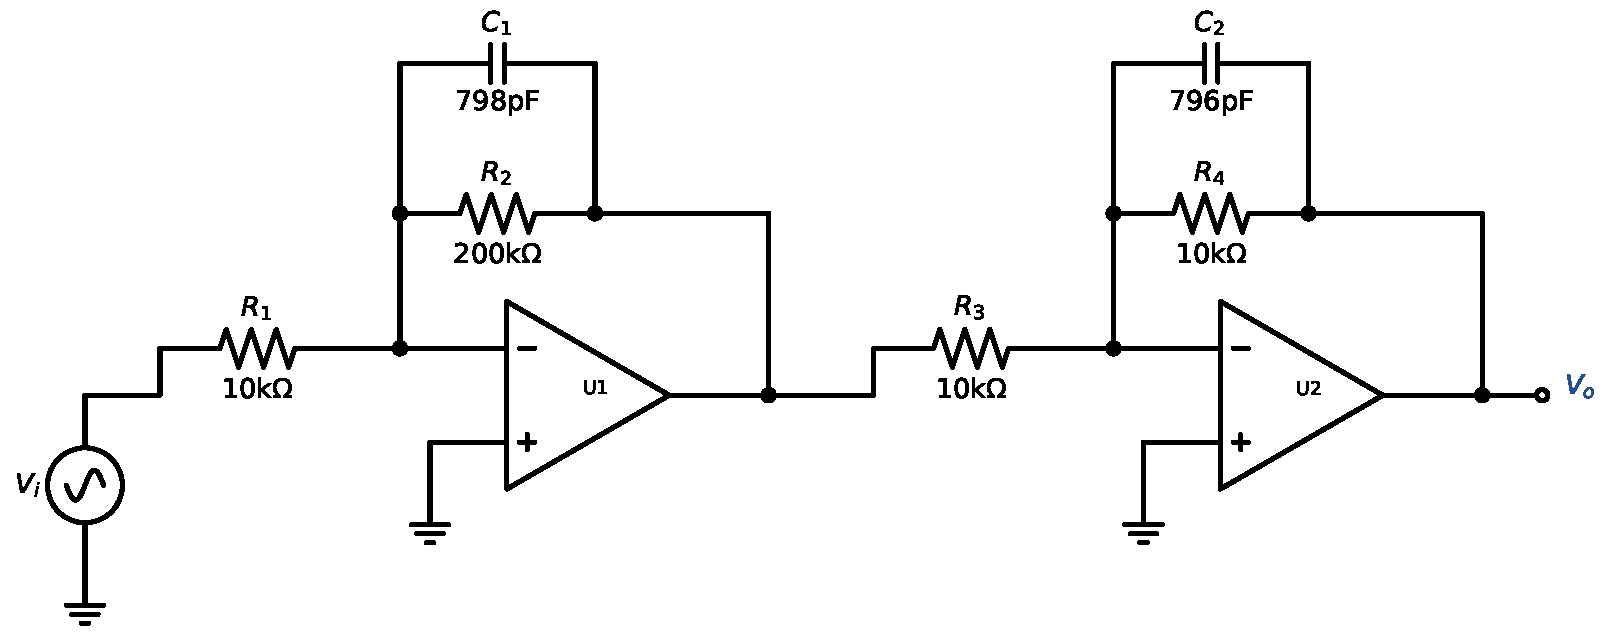
\includegraphics[width=\linewidth,height=5.5cm,keepaspectratio]{p07_design}\end{center}
Check: the stage gains multiply to $(-1)^{2}\cdot19.95\cdot(\text{factors}) = H(s)$; an independent nodal solve of this circuit reproduces $H(s)$ at every frequency. (Standard-value resistors and capacitors would move the corners slightly.)

The input is $V_i(t) = 0.05\sin\left(2\pi\cdot 5000\,t\right)$, so $\omega_{in} = 2\pi\cdot 5000 = 31400$\,rad/s. Put $s=j\omega_{in}$ in each factor (tool T5): magnitudes multiply, angles add.
{\small Rules: $\left|\frac{s}{s+p}\right| = \frac{\omega}{\sqrt{\omega^2+p^2}}$, $\angle = \frac{\pi}{2}-\tan^{-1}\frac{\omega}{p}$;\quad $\left|\frac{1}{1+s/p}\right| = \frac{1}{\sqrt{1+(\omega/p)^2}}$, $\angle = -\tan^{-1}\frac{\omega}{p}$;\quad $\left|1+\frac{s}{z}\right| = \sqrt{1+(\omega/z)^2}$, $\angle = \tan^{-1}\frac{\omega}{z}$;\quad a negative $K$ adds $-\pi$.}
\begin{center}\renewcommand{\arraystretch}{1.35}
\begin{tabular}{ccc}
\toprule
factor & magnitude & angle (rad) \\
\midrule
$20$ & $19.95$ & $0$ \\
$\rule[-1.7em]{0pt}{4em}\dfrac{1}{1+\dfrac{s}{2\pi\cdot 1\mathrm{k}}}$ & $0.1961$ & $-1.37$ \\
$\rule[-1.7em]{0pt}{4em}\dfrac{1}{1+\dfrac{s}{2\pi\cdot 20\mathrm{k}}}$ & $0.9701$ & $-0.245$ \\
\textbf{total} & $\mathbf{3.796}$ (product) & $\mathbf{-1.62}$ (sum) \\
\bottomrule
\end{tabular}\end{center}

\begin{align*}
|H(j\omega_{in})| &= 3.8, \qquad \angle H(j\omega_{in}) = -1.62\ \mathrm{rad} \\
v_{o,ac}(t) &= 3.8\times 0.05\,\sin\left(2\pi\cdot 5000\,t - 1.62\right) = 0.19\,\sin\left(2\pi\cdot 5000\,t - 1.62\right)
\end{align*}

\[
\boxed{V_o(t) = 0.19\,\sin\left(2\pi\cdot 5000\,t - 1.62\right)\ \mathrm{V}}
\]

\begin{ansbox}
$H(s) = 20\,\dfrac{1}{1+\dfrac{s}{2\pi\cdot 1\mathrm{k}}}\,\dfrac{1}{1+\dfrac{s}{2\pi\cdot 20\mathrm{k}}}$\\[4pt]
U1: R1 = 10k$\Omega$, R2 = 200k$\Omega$, C1 = 798pF\\
U2: R3 = 10k$\Omega$, R4 = 10k$\Omega$, C2 = 796pF\\[4pt]
$V_o(t) = 0.19\,\sin\left(2\pi\cdot 5000\,t - 1.62\right)\ \mathrm{V}$
\end{ansbox}

\newpage
\subsection*{Solution 2C.8 \hfill Medium}
\begin{center}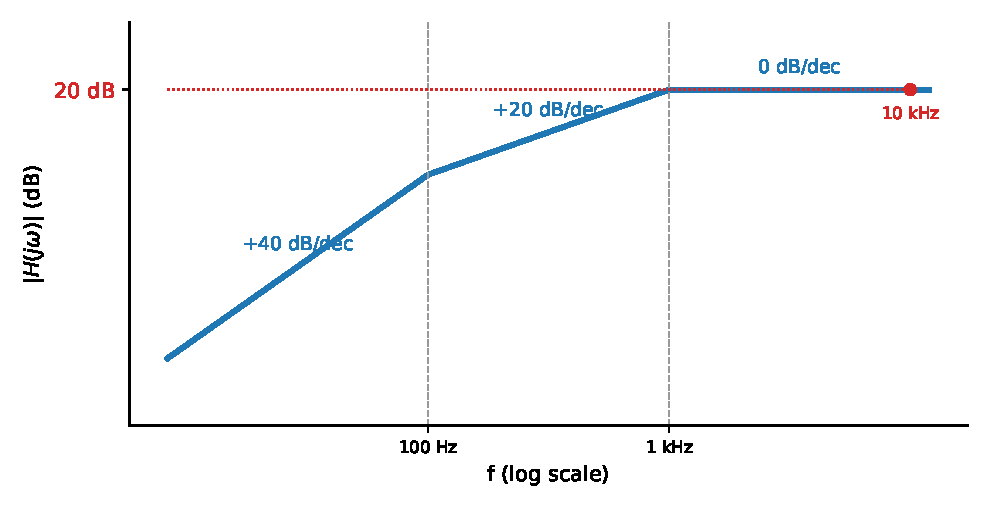
\includegraphics[width=\linewidth,height=5cm,keepaspectratio]{p08_plot}\end{center}
\solstep{1}{Read the corners and slopes}Go left to right along the plot and write down the slope of every straight segment. At each corner frequency the slope changes by a multiple of 20\,dB/dec: every $-20$ is one pole, every $+20$ is one zero (tool T6 read backwards).\begin{center}\renewcommand{\arraystretch}{1.35}
\begin{tabular}{ccccl}
\toprule
corner $f_c$ & slope before & slope after & change & meaning \\
\midrule
100 Hz & $+40$ & $+20$ & $-20$ & one pole at $f_c$ \\
1 kHz & $+20$ & $0$ & $-20$ & one pole at $f_c$ \\
\bottomrule
\end{tabular}\end{center}

\solstep{2}{Starting slope $\Rightarrow$ factors of $s$}The plot starts with a slope of $+40$\,dB/dec, i.e. $|H|\propto\omega^2$ at low frequency: the numerator contains $s^2$. As in class, pair each $s$ with one of the \emph{lowest} poles (100 Hz, 1 kHz) as $\frac{s}{s+p}$: such a factor rises at $+20$\,dB/dec below $p$ and is $\approx1$ (0\,dB) above it. The remaining poles are written $\frac{1}{1+s/p}$ and the zeros $\left(1+\frac{s}{z}\right)$. Every corner is an angular frequency $\omega_c=2\pi f_c$.
\solstep{3}{Assemble $H(s)$}Put one factor per pole/zero in front of an unknown constant $K$:\[
H(s) = K\,\dfrac{s}{s+2\pi\cdot 100}\,\dfrac{s}{s+2\pi\cdot 1\mathrm{k}}
\]

\solstep{4}{Find $K$ from the marked level}The plot marks the level $20$\,dB at $f=$\,10 kHz. On the straight-line plot every factor is either exactly 0\,dB (where it is $\approx1$) or a $\pm20$\,dB/dec line, so evaluate the \emph{asymptote} of each factor at that frequency (the level of a line with slope $\pm20$\,dB/dec is $\pm20\log_{10}(f/f_c)$):\begin{center}\renewcommand{\arraystretch}{1.35}
\begin{tabular}{cccc}
\toprule
factor & $f_c$ & at $f=$\,10 kHz & asymptote (dB) \\
\midrule
$\rule[-1.1em]{0pt}{2.8em}\dfrac{s}{s+2\pi\cdot 100}$ & 100 Hz & $f>f_c$: $\approx 1$ & $0$ \\
$\rule[-1.1em]{0pt}{2.8em}\dfrac{s}{s+2\pi\cdot 1\mathrm{k}}$ & 1 kHz & $f>f_c$: $\approx 1$ & $0$ \\
\textbf{sum} &  &  & $\mathbf{0}$ \\
\bottomrule
\end{tabular}\end{center}
The dB values of the factors \emph{add} (magnitudes multiply), so\[
20\log_{10}K = 20 - (0) = 20\ \mathrm{dB}\quad\Rightarrow\quad K = 10^{20/20} = 10
\]

So\[
\boxed{H(s) = 10\,\dfrac{s}{s+2\pi\cdot 100}\,\dfrac{s}{s+2\pi\cdot 1\mathrm{k}}}
\]


\solstep{5}{Split $H(s)$ into op-amp stages}Every inverting stage of the form $-\frac{Z_f}{Z_{in}}$ with $Z_{in}$, $Z_f$ made of one R and at most one C realizes \emph{one} pole, optionally with one zero or one $s$ (tool T2). Pair each zero with a low-pass pole (pole-zero stage), each $\frac{s}{s+p}$ with a remaining low-pass pole (band-pass stage), and give every leftover factor its own stage. Put all of $|K|$ into the first stage. Each stage inverts, so with an odd number of stages add a unity-gain inverter to make $K>0$.\begin{center}\renewcommand{\arraystretch}{1.35}
\begin{tabular}{cccl}
\toprule
stage & gain $\frac{R_2}{R_1}$ & factor(s) realized & block \\
\midrule
U1 & $10$ & $\rule[-1.4em]{0pt}{3.4em}\dfrac{s}{s+2\pi\cdot 100}$ & high-pass: $Z_{in}=R+\frac{1}{sC}$, $Z_f=R$ \\
U2 & $1$ & $\rule[-1.4em]{0pt}{3.4em}\dfrac{s}{s+2\pi\cdot 1\mathrm{k}}$ & high-pass: $Z_{in}=R+\frac{1}{sC}$, $Z_f=R$ \\
\bottomrule
\end{tabular}\end{center}

\solstep{6}{Component values}Use $R_1 = 10\,\mathrm{k}\Omega$ at the input of every stage (any convenient value works; it only scales the other parts). The corner of a factor $1+s/\omega_c$ is matched by $RC = 1/\omega_c$ (corners in rad/s).\begin{enumerate}[leftmargin=*,itemsep=2pt]
\item U1: choose $R_{1} = 10\,\mathrm{k}\Omega$, then match the stage formula $-\frac{R_{2}}{R_{1}}\cdot\frac{s}{s+1/(R_{1}C_{1})}$ to the factors:\[
C_{1} = \frac{1}{628\,R_{1}} = 159\,\mathrm{n}\mathrm{F},\qquad R_{2} = 10\,R_{1} = 100\,\mathrm{k}\Omega
\]

\item U2: choose $R_{3} = 10\,\mathrm{k}\Omega$, then match the stage formula $-\frac{R_{4}}{R_{3}}\cdot\frac{s}{s+1/(R_{3}C_{2})}$ to the factors:\[
C_{2} = \frac{1}{6280\,R_{3}} = 15.9\,\mathrm{n}\mathrm{F},\qquad R_{4} = 1\,R_{3} = 10\,\mathrm{k}\Omega
\]

\end{enumerate}

\solstep{7}{Check and steady-state output}The designed circuit:\begin{center}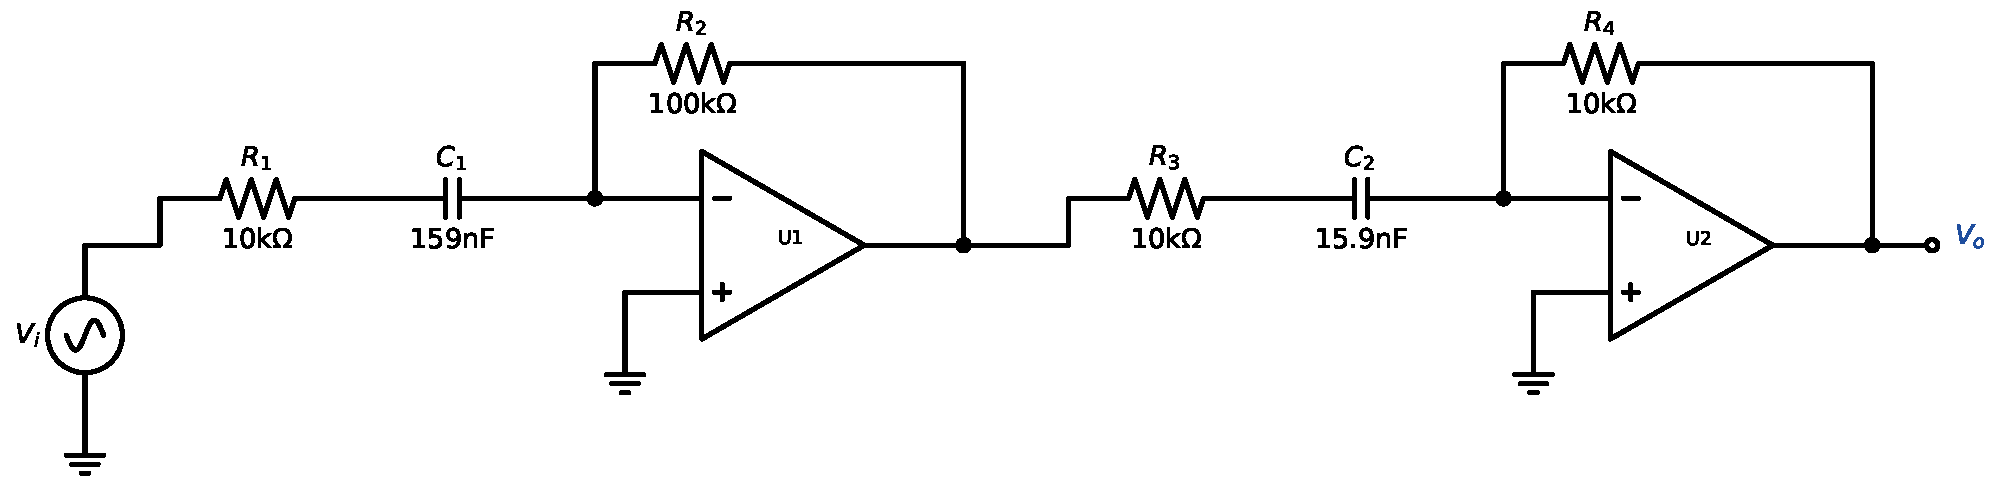
\includegraphics[width=\linewidth,height=5.5cm,keepaspectratio]{p08_design}\end{center}
Check: the stage gains multiply to $(-1)^{2}\cdot10\cdot(\text{factors}) = H(s)$; an independent nodal solve of this circuit reproduces $H(s)$ at every frequency. (Standard-value resistors and capacitors would move the corners slightly.)

The input is $V_i(t) = 0.1\sin\left(2\pi\cdot 300\,t\right)$, so $\omega_{in} = 2\pi\cdot 300 = 1880$\,rad/s. Put $s=j\omega_{in}$ in each factor (tool T5): magnitudes multiply, angles add.
{\small Rules: $\left|\frac{s}{s+p}\right| = \frac{\omega}{\sqrt{\omega^2+p^2}}$, $\angle = \frac{\pi}{2}-\tan^{-1}\frac{\omega}{p}$;\quad $\left|\frac{1}{1+s/p}\right| = \frac{1}{\sqrt{1+(\omega/p)^2}}$, $\angle = -\tan^{-1}\frac{\omega}{p}$;\quad $\left|1+\frac{s}{z}\right| = \sqrt{1+(\omega/z)^2}$, $\angle = \tan^{-1}\frac{\omega}{z}$;\quad a negative $K$ adds $-\pi$.}
\begin{center}\renewcommand{\arraystretch}{1.35}
\begin{tabular}{ccc}
\toprule
factor & magnitude & angle (rad) \\
\midrule
$10$ & $10$ & $0$ \\
$\rule[-1.1em]{0pt}{2.8em}\dfrac{s}{s+2\pi\cdot 100}$ & $0.9487$ & $0.322$ \\
$\rule[-1.1em]{0pt}{2.8em}\dfrac{s}{s+2\pi\cdot 1\mathrm{k}}$ & $0.2873$ & $1.28$ \\
\textbf{total} & $\mathbf{2.726}$ (product) & $\mathbf{1.6}$ (sum) \\
\bottomrule
\end{tabular}\end{center}

\begin{align*}
|H(j\omega_{in})| &= 2.73, \qquad \angle H(j\omega_{in}) = 1.6\ \mathrm{rad} \\
v_{o,ac}(t) &= 2.73\times 0.1\,\sin\left(2\pi\cdot 300\,t + 1.6\right) = 0.273\,\sin\left(2\pi\cdot 300\,t + 1.6\right)
\end{align*}

\[
\boxed{V_o(t) = 0.273\,\sin\left(2\pi\cdot 300\,t + 1.6\right)\ \mathrm{V}}
\]

\begin{ansbox}
$H(s) = 10\,\dfrac{s}{s+2\pi\cdot 100}\,\dfrac{s}{s+2\pi\cdot 1\mathrm{k}}$\\[4pt]
U1: R1 = 10k$\Omega$, C1 = 159nF, R2 = 100k$\Omega$\\
U2: R3 = 10k$\Omega$, C2 = 15.9nF, R4 = 10k$\Omega$\\[4pt]
$V_o(t) = 0.273\,\sin\left(2\pi\cdot 300\,t + 1.6\right)\ \mathrm{V}$
\end{ansbox}

\newpage
\subsection*{Solution 2C.9 \hfill Medium}
\begin{center}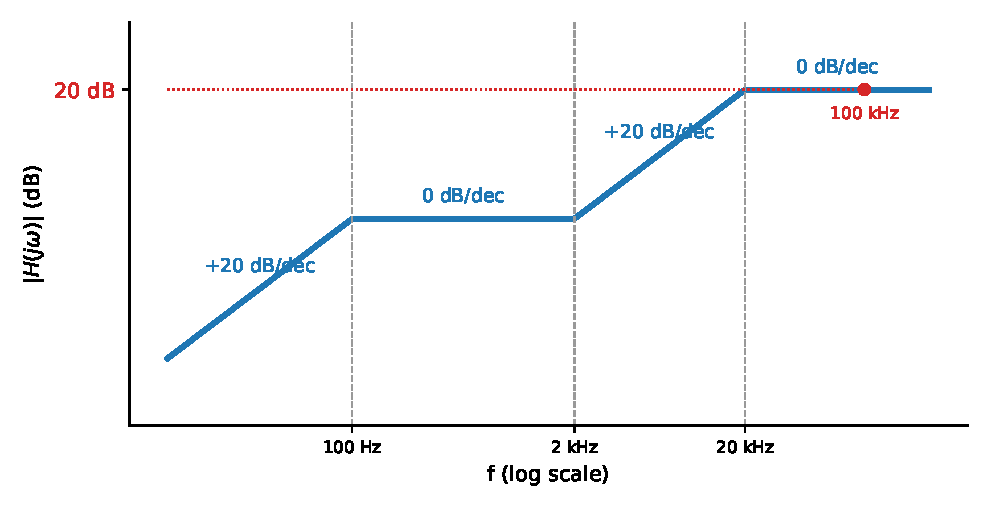
\includegraphics[width=\linewidth,height=5cm,keepaspectratio]{p09_plot}\end{center}
\solstep{1}{Read the corners and slopes}Go left to right along the plot and write down the slope of every straight segment. At each corner frequency the slope changes by a multiple of 20\,dB/dec: every $-20$ is one pole, every $+20$ is one zero (tool T6 read backwards).\begin{center}\renewcommand{\arraystretch}{1.35}
\begin{tabular}{ccccl}
\toprule
corner $f_c$ & slope before & slope after & change & meaning \\
\midrule
100 Hz & $+20$ & $0$ & $-20$ & one pole at $f_c$ \\
2 kHz & $0$ & $+20$ & $+20$ & one zero at $f_c$ \\
20 kHz & $+20$ & $0$ & $-20$ & one pole at $f_c$ \\
\bottomrule
\end{tabular}\end{center}

\solstep{2}{Starting slope $\Rightarrow$ factors of $s$}The plot starts with a slope of $+20$\,dB/dec, i.e. $|H|\propto\omega^1$ at low frequency: the numerator contains $s$. As in class, pair each $s$ with one of the \emph{lowest} poles (100 Hz) as $\frac{s}{s+p}$: such a factor rises at $+20$\,dB/dec below $p$ and is $\approx1$ (0\,dB) above it. The remaining poles are written $\frac{1}{1+s/p}$ and the zeros $\left(1+\frac{s}{z}\right)$. Every corner is an angular frequency $\omega_c=2\pi f_c$.
\solstep{3}{Assemble $H(s)$}Put one factor per pole/zero in front of an unknown constant $K$:\[
H(s) = K\,\dfrac{s}{s+2\pi\cdot 100}\,\left(1+\dfrac{s}{2\pi\cdot 2\mathrm{k}}\right)\,\dfrac{1}{1+\dfrac{s}{2\pi\cdot 20\mathrm{k}}}
\]

\solstep{4}{Find $K$ from the marked level}The plot marks the level $20$\,dB at $f=$\,100 kHz. On the straight-line plot every factor is either exactly 0\,dB (where it is $\approx1$) or a $\pm20$\,dB/dec line, so evaluate the \emph{asymptote} of each factor at that frequency (the level of a line with slope $\pm20$\,dB/dec is $\pm20\log_{10}(f/f_c)$):\begin{center}\renewcommand{\arraystretch}{1.35}
\begin{tabular}{cccc}
\toprule
factor & $f_c$ & at $f=$\,100 kHz & asymptote (dB) \\
\midrule
$\rule[-1.1em]{0pt}{2.8em}\dfrac{s}{s+2\pi\cdot 100}$ & 100 Hz & $f>f_c$: $\approx 1$ & $0$ \\
$\rule[-1.1em]{0pt}{2.8em}\left(1+\dfrac{s}{2\pi\cdot 2\mathrm{k}}\right)$ & 2 kHz & $f>f_c$: $\approx \frac{\omega}{z}$ & $34$ \\
$\rule[-1.7em]{0pt}{4em}\dfrac{1}{1+\dfrac{s}{2\pi\cdot 20\mathrm{k}}}$ & 20 kHz & $f>f_c$: $\approx \frac{p}{\omega}$ & $-14$ \\
\textbf{sum} &  &  & $\mathbf{20}$ \\
\bottomrule
\end{tabular}\end{center}
The dB values of the factors \emph{add} (magnitudes multiply), so\[
20\log_{10}K = 20 - (20) = 0\ \mathrm{dB}\quad\Rightarrow\quad K = 10^{0/20} = 1
\]

So\[
\boxed{H(s) = 1\,\dfrac{s}{s+2\pi\cdot 100}\,\left(1+\dfrac{s}{2\pi\cdot 2\mathrm{k}}\right)\,\dfrac{1}{1+\dfrac{s}{2\pi\cdot 20\mathrm{k}}}}
\]


\solstep{5}{Split $H(s)$ into op-amp stages}Every inverting stage of the form $-\frac{Z_f}{Z_{in}}$ with $Z_{in}$, $Z_f$ made of one R and at most one C realizes \emph{one} pole, optionally with one zero or one $s$ (tool T2). Pair each zero with a low-pass pole (pole-zero stage), each $\frac{s}{s+p}$ with a remaining low-pass pole (band-pass stage), and give every leftover factor its own stage. Put all of $|K|$ into the first stage. Each stage inverts, so with an odd number of stages add a unity-gain inverter to make $K>0$.\begin{center}\renewcommand{\arraystretch}{1.35}
\begin{tabular}{cccl}
\toprule
stage & gain $\frac{R_2}{R_1}$ & factor(s) realized & block \\
\midrule
U1 & $1$ & $\rule[-1.4em]{0pt}{3.4em}\dfrac{s}{s+2\pi\cdot 100}$ & high-pass: $Z_{in}=R+\frac{1}{sC}$, $Z_f=R$ \\
U2 & $1$ & $\rule[-1.4em]{0pt}{3.4em}\dfrac{1+\frac{s}{2\pi\cdot 2\mathrm{k}}}{1+\frac{s}{2\pi\cdot 20\mathrm{k}}}$ & pole-zero: $Z_{in}=R\parallel C$, $Z_f = R\parallel C$ \\
\bottomrule
\end{tabular}\end{center}

\solstep{6}{Component values}Use $R_1 = 10\,\mathrm{k}\Omega$ at the input of every stage (any convenient value works; it only scales the other parts). The corner of a factor $1+s/\omega_c$ is matched by $RC = 1/\omega_c$ (corners in rad/s).\begin{enumerate}[leftmargin=*,itemsep=2pt]
\item U1: choose $R_{1} = 10\,\mathrm{k}\Omega$, then match the stage formula $-\frac{R_{2}}{R_{1}}\cdot\frac{s}{s+1/(R_{1}C_{1})}$ to the factors:\[
C_{1} = \frac{1}{628\,R_{1}} = 159\,\mathrm{n}\mathrm{F},\qquad R_{2} = 1\,R_{1} = 10\,\mathrm{k}\Omega
\]

\item U2: choose $R_{3} = 10\,\mathrm{k}\Omega$, then match the stage formula $-\frac{R_{4}}{R_{3}}\cdot\frac{1+sR_{3}C_{2}}{1+sR_{4}C_{3}}$ to the factors:\[
R_{4} = 1\,R_{3} = 10\,\mathrm{k}\Omega,\qquad C_{2} = \frac{1}{12600\,R_{3}} = 7.96\,\mathrm{n}\mathrm{F},\qquad C_{3} = \frac{1}{1.26\times 10^{5}\,R_{4}} = 796\,\mathrm{p}\mathrm{F}
\]

\end{enumerate}

\solstep{7}{Check and steady-state output}The designed circuit:\begin{center}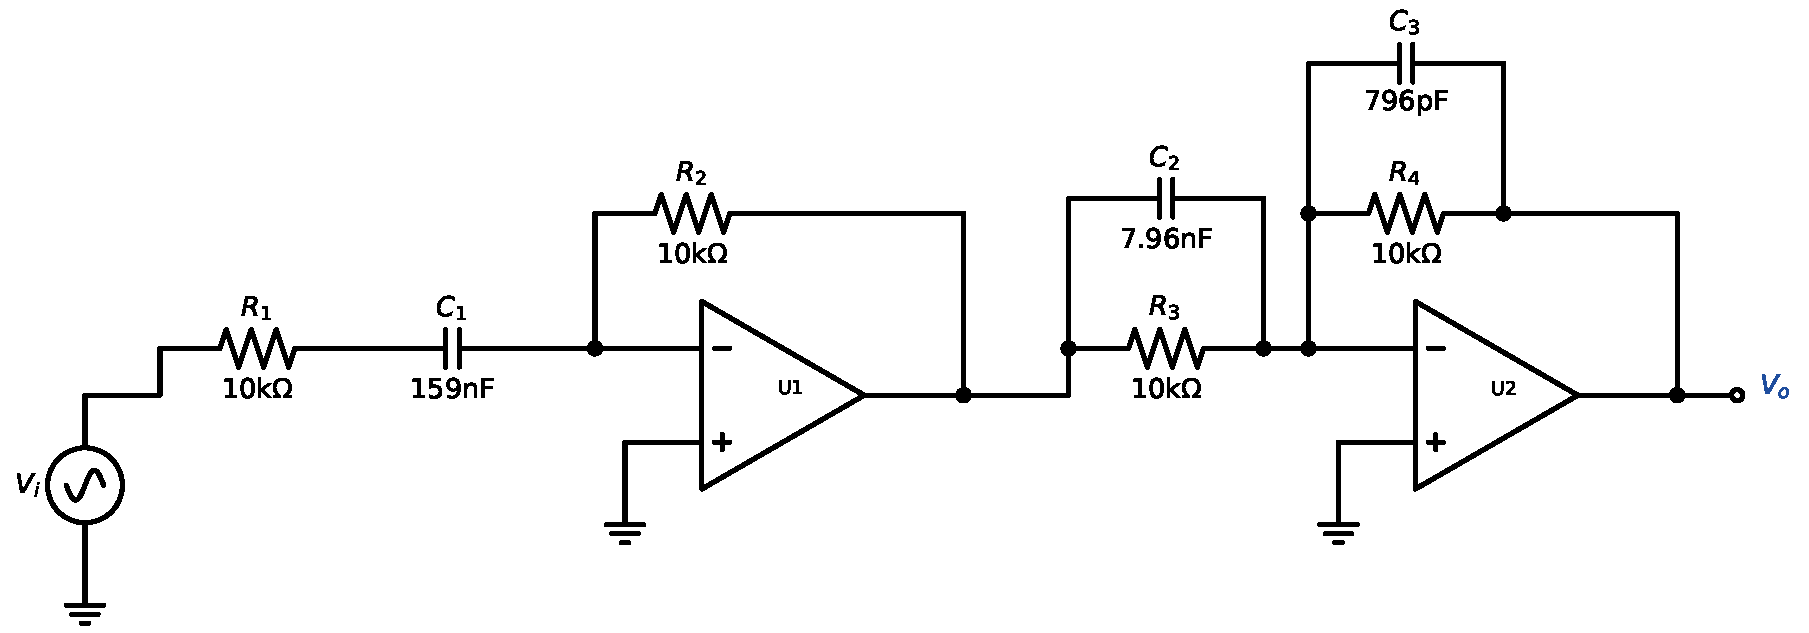
\includegraphics[width=\linewidth,height=5.5cm,keepaspectratio]{p09_design}\end{center}
Check: the stage gains multiply to $(-1)^{2}\cdot1\cdot(\text{factors}) = H(s)$; an independent nodal solve of this circuit reproduces $H(s)$ at every frequency. (Standard-value resistors and capacitors would move the corners slightly.)

The input is $V_i(t) = 0.2\sin\left(2\pi\cdot 1000\,t\right)$, so $\omega_{in} = 2\pi\cdot 1000 = 6280$\,rad/s. Put $s=j\omega_{in}$ in each factor (tool T5): magnitudes multiply, angles add.
{\small Rules: $\left|\frac{s}{s+p}\right| = \frac{\omega}{\sqrt{\omega^2+p^2}}$, $\angle = \frac{\pi}{2}-\tan^{-1}\frac{\omega}{p}$;\quad $\left|\frac{1}{1+s/p}\right| = \frac{1}{\sqrt{1+(\omega/p)^2}}$, $\angle = -\tan^{-1}\frac{\omega}{p}$;\quad $\left|1+\frac{s}{z}\right| = \sqrt{1+(\omega/z)^2}$, $\angle = \tan^{-1}\frac{\omega}{z}$;\quad a negative $K$ adds $-\pi$.}
\begin{center}\renewcommand{\arraystretch}{1.35}
\begin{tabular}{ccc}
\toprule
factor & magnitude & angle (rad) \\
\midrule
$1$ & $1$ & $0$ \\
$\rule[-1.1em]{0pt}{2.8em}\dfrac{s}{s+2\pi\cdot 100}$ & $0.995$ & $0.0997$ \\
$\rule[-1.1em]{0pt}{2.8em}\left(1+\dfrac{s}{2\pi\cdot 2\mathrm{k}}\right)$ & $1.118$ & $0.464$ \\
$\rule[-1.7em]{0pt}{4em}\dfrac{1}{1+\dfrac{s}{2\pi\cdot 20\mathrm{k}}}$ & $0.9988$ & $-0.05$ \\
\textbf{total} & $\mathbf{1.111}$ (product) & $\mathbf{0.513}$ (sum) \\
\bottomrule
\end{tabular}\end{center}

\begin{align*}
|H(j\omega_{in})| &= 1.11, \qquad \angle H(j\omega_{in}) = 0.513\ \mathrm{rad} \\
v_{o,ac}(t) &= 1.11\times 0.2\,\sin\left(2\pi\cdot 1000\,t + 0.513\right) = 0.222\,\sin\left(2\pi\cdot 1000\,t + 0.513\right)
\end{align*}

\[
\boxed{V_o(t) = 0.222\,\sin\left(2\pi\cdot 1000\,t + 0.513\right)\ \mathrm{V}}
\]

\begin{ansbox}
$H(s) = 1\,\dfrac{s}{s+2\pi\cdot 100}\,\left(1+\dfrac{s}{2\pi\cdot 2\mathrm{k}}\right)\,\dfrac{1}{1+\dfrac{s}{2\pi\cdot 20\mathrm{k}}}$\\[4pt]
U1: R1 = 10k$\Omega$, C1 = 159nF, R2 = 10k$\Omega$\\
U2: R3 = 10k$\Omega$, C2 = 7.96nF, R4 = 10k$\Omega$, C3 = 796pF\\[4pt]
$V_o(t) = 0.222\,\sin\left(2\pi\cdot 1000\,t + 0.513\right)\ \mathrm{V}$
\end{ansbox}

\newpage
\subsection*{Solution 2C.10 \hfill Medium}
\begin{center}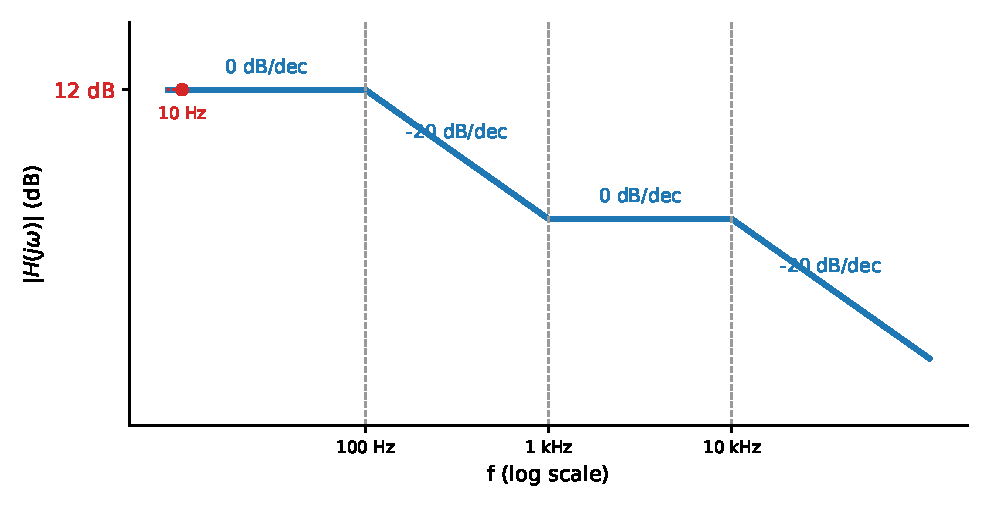
\includegraphics[width=\linewidth,height=5cm,keepaspectratio]{p10_plot}\end{center}
\solstep{1}{Read the corners and slopes}Go left to right along the plot and write down the slope of every straight segment. At each corner frequency the slope changes by a multiple of 20\,dB/dec: every $-20$ is one pole, every $+20$ is one zero (tool T6 read backwards).\begin{center}\renewcommand{\arraystretch}{1.35}
\begin{tabular}{ccccl}
\toprule
corner $f_c$ & slope before & slope after & change & meaning \\
\midrule
100 Hz & $0$ & $-20$ & $-20$ & one pole at $f_c$ \\
1 kHz & $-20$ & $0$ & $+20$ & one zero at $f_c$ \\
10 kHz & $0$ & $-20$ & $-20$ & one pole at $f_c$ \\
\bottomrule
\end{tabular}\end{center}

\solstep{2}{Starting slope $\Rightarrow$ factors of $s$}The plot starts \emph{flat} (0\,dB/dec), so there is no factor $s$ in the numerator: every pole is written as $\frac{1}{1+s/p}$ and every zero as $\left(1+\frac{s}{z}\right)$, which are all $\approx1$ (0\,dB) at low frequency. Every corner is an angular frequency $\omega_c=2\pi f_c$.
\solstep{3}{Assemble $H(s)$}Put one factor per pole/zero in front of an unknown constant $K$:\[
H(s) = K\,\dfrac{1}{1+\dfrac{s}{2\pi\cdot 100}}\,\left(1+\dfrac{s}{2\pi\cdot 1\mathrm{k}}\right)\,\dfrac{1}{1+\dfrac{s}{2\pi\cdot 10\mathrm{k}}}
\]

\solstep{4}{Find $K$ from the marked level}The plot marks the level $12$\,dB at $f=$\,10 Hz. On the straight-line plot every factor is either exactly 0\,dB (where it is $\approx1$) or a $\pm20$\,dB/dec line, so evaluate the \emph{asymptote} of each factor at that frequency (the level of a line with slope $\pm20$\,dB/dec is $\pm20\log_{10}(f/f_c)$):\begin{center}\renewcommand{\arraystretch}{1.35}
\begin{tabular}{cccc}
\toprule
factor & $f_c$ & at $f=$\,10 Hz & asymptote (dB) \\
\midrule
$\rule[-1.7em]{0pt}{4em}\dfrac{1}{1+\dfrac{s}{2\pi\cdot 100}}$ & 100 Hz & $f<f_c$: $\approx 1$ & $0$ \\
$\rule[-1.1em]{0pt}{2.8em}\left(1+\dfrac{s}{2\pi\cdot 1\mathrm{k}}\right)$ & 1 kHz & $f<f_c$: $\approx 1$ & $0$ \\
$\rule[-1.7em]{0pt}{4em}\dfrac{1}{1+\dfrac{s}{2\pi\cdot 10\mathrm{k}}}$ & 10 kHz & $f<f_c$: $\approx 1$ & $0$ \\
\textbf{sum} &  &  & $\mathbf{0}$ \\
\bottomrule
\end{tabular}\end{center}
The dB values of the factors \emph{add} (magnitudes multiply), so\[
20\log_{10}K = 12 - (0) = 12\ \mathrm{dB}\quad\Rightarrow\quad K = 10^{12/20} = 3.98
\]

So\[
\boxed{H(s) = 3.98\,\dfrac{1}{1+\dfrac{s}{2\pi\cdot 100}}\,\left(1+\dfrac{s}{2\pi\cdot 1\mathrm{k}}\right)\,\dfrac{1}{1+\dfrac{s}{2\pi\cdot 10\mathrm{k}}}}
\]


\solstep{5}{Split $H(s)$ into op-amp stages}Every inverting stage of the form $-\frac{Z_f}{Z_{in}}$ with $Z_{in}$, $Z_f$ made of one R and at most one C realizes \emph{one} pole, optionally with one zero or one $s$ (tool T2). Pair each zero with a low-pass pole (pole-zero stage), each $\frac{s}{s+p}$ with a remaining low-pass pole (band-pass stage), and give every leftover factor its own stage. Put all of $|K|$ into the first stage. Each stage inverts, so with an odd number of stages add a unity-gain inverter to make $K>0$.\begin{center}\renewcommand{\arraystretch}{1.35}
\begin{tabular}{cccl}
\toprule
stage & gain $\frac{R_2}{R_1}$ & factor(s) realized & block \\
\midrule
U1 & $3.981$ & $\rule[-1.4em]{0pt}{3.4em}\dfrac{1+\frac{s}{2\pi\cdot 1\mathrm{k}}}{1+\frac{s}{2\pi\cdot 100}}$ & pole-zero: $Z_{in}=R\parallel C$, $Z_f = R\parallel C$ \\
U2 & $1$ & $\rule[-1.4em]{0pt}{3.4em}\dfrac{1}{1+\frac{s}{2\pi\cdot 10\mathrm{k}}}$ & low-pass: $Z_{in}=R$, $Z_f=R\parallel C$ \\
\bottomrule
\end{tabular}\end{center}

\solstep{6}{Component values}Use $R_1 = 10\,\mathrm{k}\Omega$ at the input of every stage (any convenient value works; it only scales the other parts). The corner of a factor $1+s/\omega_c$ is matched by $RC = 1/\omega_c$ (corners in rad/s).\begin{enumerate}[leftmargin=*,itemsep=2pt]
\item U1: choose $R_{1} = 10\,\mathrm{k}\Omega$, then match the stage formula $-\frac{R_{2}}{R_{1}}\cdot\frac{1+sR_{1}C_{1}}{1+sR_{2}C_{2}}$ to the factors:\[
R_{2} = 3.981\,R_{1} = 39.8\,\mathrm{k}\Omega,\qquad C_{1} = \frac{1}{6280\,R_{1}} = 15.9\,\mathrm{n}\mathrm{F},\qquad C_{2} = \frac{1}{628\,R_{2}} = 40\,\mathrm{n}\mathrm{F}
\]

\item U2: choose $R_{3} = 10\,\mathrm{k}\Omega$, then match the stage formula $-\frac{R_{4}}{R_{3}}\cdot\frac{1}{1+sR_{4}C_{3}}$ to the factors:\[
R_{4} = 1\,R_{3} = 10\,\mathrm{k}\Omega,\qquad C_{3} = \frac{1}{62800\,R_{4}} = 1.59\,\mathrm{n}\mathrm{F}
\]

\end{enumerate}

\solstep{7}{Check and steady-state output}The designed circuit:\begin{center}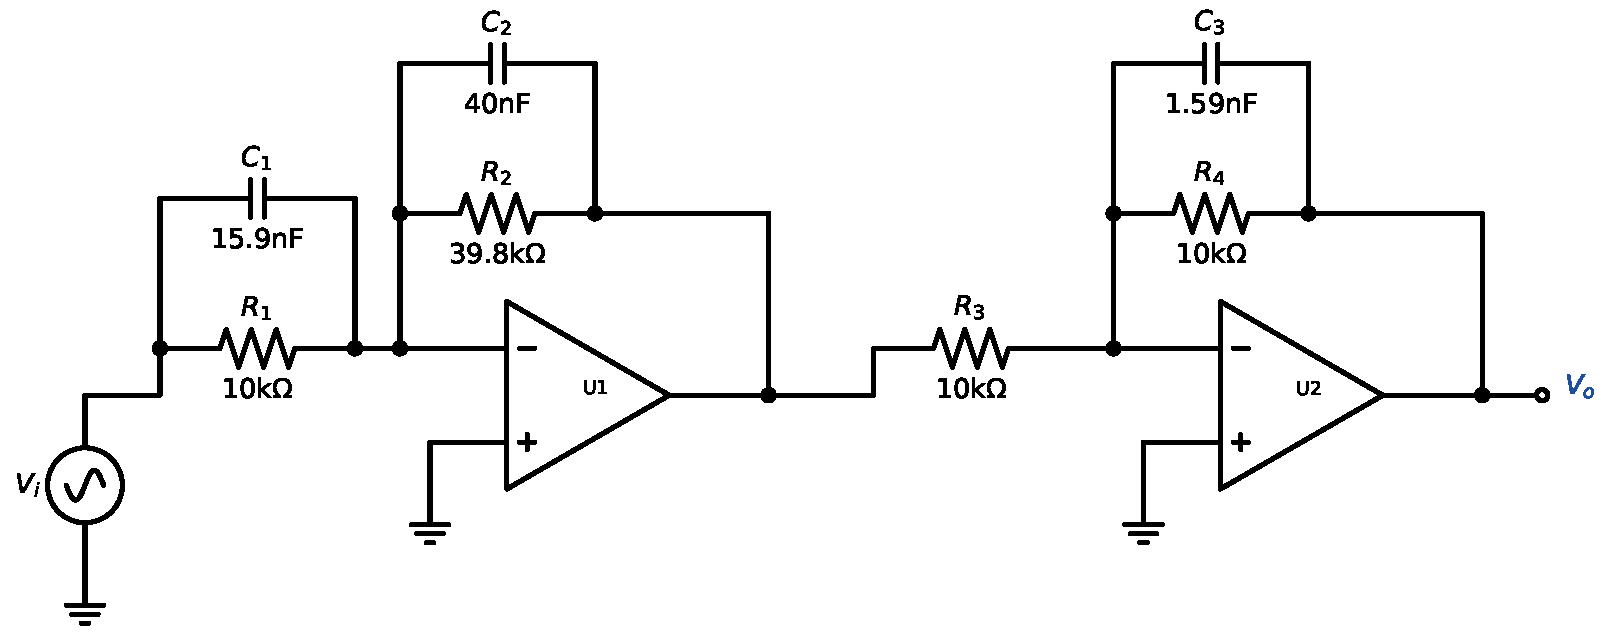
\includegraphics[width=\linewidth,height=5.5cm,keepaspectratio]{p10_design}\end{center}
Check: the stage gains multiply to $(-1)^{2}\cdot3.981\cdot(\text{factors}) = H(s)$; an independent nodal solve of this circuit reproduces $H(s)$ at every frequency. (Standard-value resistors and capacitors would move the corners slightly.)

The input is $V_i(t) = 0.2\sin\left(2\pi\cdot 2000\,t\right)$, so $\omega_{in} = 2\pi\cdot 2000 = 12600$\,rad/s. Put $s=j\omega_{in}$ in each factor (tool T5): magnitudes multiply, angles add.
{\small Rules: $\left|\frac{s}{s+p}\right| = \frac{\omega}{\sqrt{\omega^2+p^2}}$, $\angle = \frac{\pi}{2}-\tan^{-1}\frac{\omega}{p}$;\quad $\left|\frac{1}{1+s/p}\right| = \frac{1}{\sqrt{1+(\omega/p)^2}}$, $\angle = -\tan^{-1}\frac{\omega}{p}$;\quad $\left|1+\frac{s}{z}\right| = \sqrt{1+(\omega/z)^2}$, $\angle = \tan^{-1}\frac{\omega}{z}$;\quad a negative $K$ adds $-\pi$.}
\begin{center}\renewcommand{\arraystretch}{1.35}
\begin{tabular}{ccc}
\toprule
factor & magnitude & angle (rad) \\
\midrule
$3.98$ & $3.981$ & $0$ \\
$\rule[-1.7em]{0pt}{4em}\dfrac{1}{1+\dfrac{s}{2\pi\cdot 100}}$ & $0.04994$ & $-1.52$ \\
$\rule[-1.1em]{0pt}{2.8em}\left(1+\dfrac{s}{2\pi\cdot 1\mathrm{k}}\right)$ & $2.236$ & $1.11$ \\
$\rule[-1.7em]{0pt}{4em}\dfrac{1}{1+\dfrac{s}{2\pi\cdot 10\mathrm{k}}}$ & $0.9806$ & $-0.197$ \\
\textbf{total} & $\mathbf{0.4359}$ (product) & $\mathbf{-0.611}$ (sum) \\
\bottomrule
\end{tabular}\end{center}

\begin{align*}
|H(j\omega_{in})| &= 0.436, \qquad \angle H(j\omega_{in}) = -0.611\ \mathrm{rad} \\
v_{o,ac}(t) &= 0.436\times 0.2\,\sin\left(2\pi\cdot 2000\,t - 0.611\right) = 0.0872\,\sin\left(2\pi\cdot 2000\,t - 0.611\right)
\end{align*}

\[
\boxed{V_o(t) = 0.0872\,\sin\left(2\pi\cdot 2000\,t - 0.611\right)\ \mathrm{V}}
\]

\begin{ansbox}
$H(s) = 3.98\,\dfrac{1}{1+\dfrac{s}{2\pi\cdot 100}}\,\left(1+\dfrac{s}{2\pi\cdot 1\mathrm{k}}\right)\,\dfrac{1}{1+\dfrac{s}{2\pi\cdot 10\mathrm{k}}}$\\[4pt]
U1: R1 = 10k$\Omega$, C1 = 15.9nF, R2 = 39.8k$\Omega$, C2 = 40nF\\
U2: R3 = 10k$\Omega$, R4 = 10k$\Omega$, C3 = 1.59nF\\[4pt]
$V_o(t) = 0.0872\,\sin\left(2\pi\cdot 2000\,t - 0.611\right)\ \mathrm{V}$
\end{ansbox}

\newpage
\subsection*{Solution 2C.11 \hfill Medium}
\begin{center}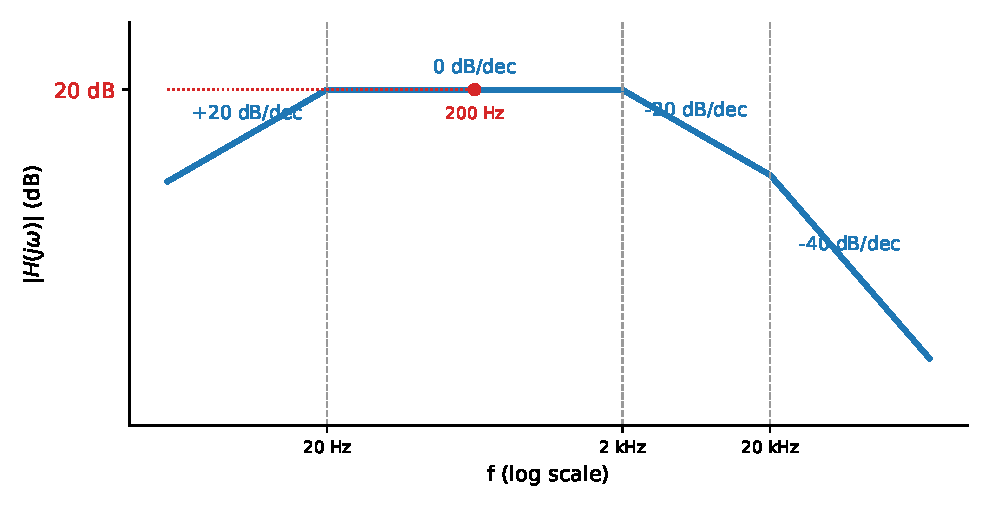
\includegraphics[width=\linewidth,height=5cm,keepaspectratio]{p11_plot}\end{center}
\solstep{1}{Read the corners and slopes}Go left to right along the plot and write down the slope of every straight segment. At each corner frequency the slope changes by a multiple of 20\,dB/dec: every $-20$ is one pole, every $+20$ is one zero (tool T6 read backwards).\begin{center}\renewcommand{\arraystretch}{1.35}
\begin{tabular}{ccccl}
\toprule
corner $f_c$ & slope before & slope after & change & meaning \\
\midrule
20 Hz & $+20$ & $0$ & $-20$ & one pole at $f_c$ \\
2 kHz & $0$ & $-20$ & $-20$ & one pole at $f_c$ \\
20 kHz & $-20$ & $-40$ & $-20$ & one pole at $f_c$ \\
\bottomrule
\end{tabular}\end{center}

\solstep{2}{Starting slope $\Rightarrow$ factors of $s$}The plot starts with a slope of $+20$\,dB/dec, i.e. $|H|\propto\omega^1$ at low frequency: the numerator contains $s$. As in class, pair each $s$ with one of the \emph{lowest} poles (20 Hz) as $\frac{s}{s+p}$: such a factor rises at $+20$\,dB/dec below $p$ and is $\approx1$ (0\,dB) above it. The remaining poles are written $\frac{1}{1+s/p}$ and the zeros $\left(1+\frac{s}{z}\right)$. Every corner is an angular frequency $\omega_c=2\pi f_c$.
\solstep{3}{Assemble $H(s)$}Put one factor per pole/zero in front of an unknown constant $K$:\[
H(s) = K\,\dfrac{s}{s+2\pi\cdot 20}\,\dfrac{1}{1+\dfrac{s}{2\pi\cdot 2\mathrm{k}}}\,\dfrac{1}{1+\dfrac{s}{2\pi\cdot 20\mathrm{k}}}
\]

\solstep{4}{Find $K$ from the marked level}The plot marks the level $20$\,dB at $f=$\,200 Hz. On the straight-line plot every factor is either exactly 0\,dB (where it is $\approx1$) or a $\pm20$\,dB/dec line, so evaluate the \emph{asymptote} of each factor at that frequency (the level of a line with slope $\pm20$\,dB/dec is $\pm20\log_{10}(f/f_c)$):\begin{center}\renewcommand{\arraystretch}{1.35}
\begin{tabular}{cccc}
\toprule
factor & $f_c$ & at $f=$\,200 Hz & asymptote (dB) \\
\midrule
$\rule[-1.1em]{0pt}{2.8em}\dfrac{s}{s+2\pi\cdot 20}$ & 20 Hz & $f>f_c$: $\approx 1$ & $0$ \\
$\rule[-1.7em]{0pt}{4em}\dfrac{1}{1+\dfrac{s}{2\pi\cdot 2\mathrm{k}}}$ & 2 kHz & $f<f_c$: $\approx 1$ & $0$ \\
$\rule[-1.7em]{0pt}{4em}\dfrac{1}{1+\dfrac{s}{2\pi\cdot 20\mathrm{k}}}$ & 20 kHz & $f<f_c$: $\approx 1$ & $0$ \\
\textbf{sum} &  &  & $\mathbf{0}$ \\
\bottomrule
\end{tabular}\end{center}
The dB values of the factors \emph{add} (magnitudes multiply), so\[
20\log_{10}K = 20 - (0) = 20\ \mathrm{dB}\quad\Rightarrow\quad K = 10^{20/20} = 10
\]

So\[
\boxed{H(s) = 10\,\dfrac{s}{s+2\pi\cdot 20}\,\dfrac{1}{1+\dfrac{s}{2\pi\cdot 2\mathrm{k}}}\,\dfrac{1}{1+\dfrac{s}{2\pi\cdot 20\mathrm{k}}}}
\]


\solstep{5}{Split $H(s)$ into op-amp stages}Every inverting stage of the form $-\frac{Z_f}{Z_{in}}$ with $Z_{in}$, $Z_f$ made of one R and at most one C realizes \emph{one} pole, optionally with one zero or one $s$ (tool T2). Pair each zero with a low-pass pole (pole-zero stage), each $\frac{s}{s+p}$ with a remaining low-pass pole (band-pass stage), and give every leftover factor its own stage. Put all of $|K|$ into the first stage. Each stage inverts, so with an odd number of stages add a unity-gain inverter to make $K>0$.\begin{center}\renewcommand{\arraystretch}{1.35}
\begin{tabular}{cccl}
\toprule
stage & gain $\frac{R_2}{R_1}$ & factor(s) realized & block \\
\midrule
U1 & $10$ & $\rule[-1.4em]{0pt}{3.4em}\dfrac{s}{s+2\pi\cdot 20}\cdot\dfrac{1}{1+\frac{s}{2\pi\cdot 2\mathrm{k}}}$ & band-pass: $Z_{in}=R+\frac{1}{sC}$, $Z_f=R\parallel C$ \\
U2 & $1$ & $\rule[-1.4em]{0pt}{3.4em}\dfrac{1}{1+\frac{s}{2\pi\cdot 20\mathrm{k}}}$ & low-pass: $Z_{in}=R$, $Z_f=R\parallel C$ \\
\bottomrule
\end{tabular}\end{center}

\solstep{6}{Component values}Use $R_1 = 10\,\mathrm{k}\Omega$ at the input of every stage (any convenient value works; it only scales the other parts). The corner of a factor $1+s/\omega_c$ is matched by $RC = 1/\omega_c$ (corners in rad/s).\begin{enumerate}[leftmargin=*,itemsep=2pt]
\item U1: choose $R_{1} = 10\,\mathrm{k}\Omega$, then match the stage formula $-\frac{R_{2}}{R_{1}}\cdot\frac{s}{s+1/(R_{1}C_{1})}\cdot\frac{1}{1+sR_{2}C_{2}}$ to the factors:\[
C_{1} = \frac{1}{126\,R_{1}} = 796\,\mathrm{n}\mathrm{F},\qquad R_{2} = 10\,R_{1} = 100\,\mathrm{k}\Omega,\qquad C_{2} = \frac{1}{12600\,R_{2}} = 796\,\mathrm{p}\mathrm{F}
\]

\item U2: choose $R_{3} = 10\,\mathrm{k}\Omega$, then match the stage formula $-\frac{R_{4}}{R_{3}}\cdot\frac{1}{1+sR_{4}C_{3}}$ to the factors:\[
R_{4} = 1\,R_{3} = 10\,\mathrm{k}\Omega,\qquad C_{3} = \frac{1}{1.26\times 10^{5}\,R_{4}} = 796\,\mathrm{p}\mathrm{F}
\]

\end{enumerate}

\solstep{7}{Check and steady-state output}The designed circuit:\begin{center}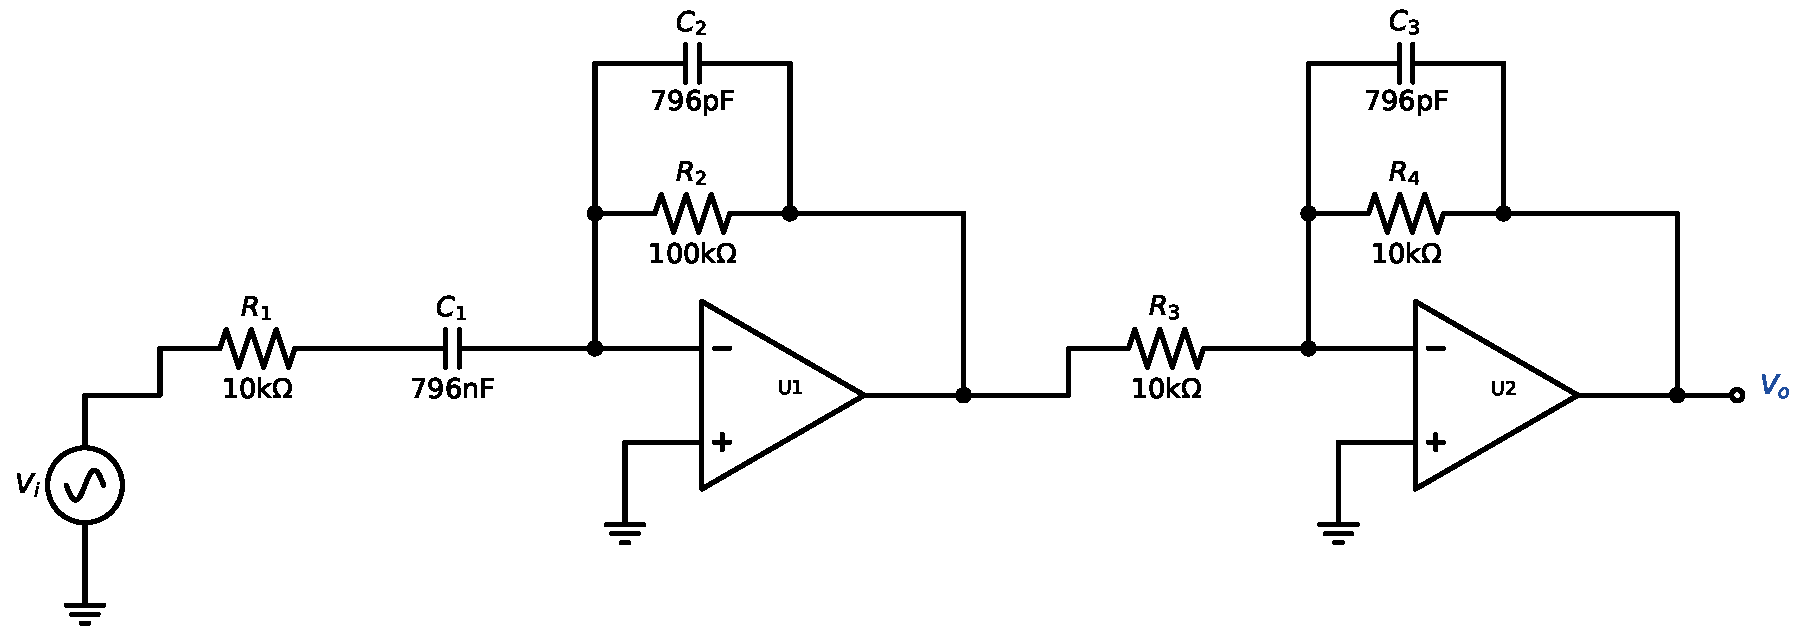
\includegraphics[width=\linewidth,height=5.5cm,keepaspectratio]{p11_design}\end{center}
Check: the stage gains multiply to $(-1)^{2}\cdot10\cdot(\text{factors}) = H(s)$; an independent nodal solve of this circuit reproduces $H(s)$ at every frequency. (Standard-value resistors and capacitors would move the corners slightly.)

The input is $V_i(t) = 0.1\sin\left(2\pi\cdot 5000\,t\right)$, so $\omega_{in} = 2\pi\cdot 5000 = 31400$\,rad/s. Put $s=j\omega_{in}$ in each factor (tool T5): magnitudes multiply, angles add.
{\small Rules: $\left|\frac{s}{s+p}\right| = \frac{\omega}{\sqrt{\omega^2+p^2}}$, $\angle = \frac{\pi}{2}-\tan^{-1}\frac{\omega}{p}$;\quad $\left|\frac{1}{1+s/p}\right| = \frac{1}{\sqrt{1+(\omega/p)^2}}$, $\angle = -\tan^{-1}\frac{\omega}{p}$;\quad $\left|1+\frac{s}{z}\right| = \sqrt{1+(\omega/z)^2}$, $\angle = \tan^{-1}\frac{\omega}{z}$;\quad a negative $K$ adds $-\pi$.}
\begin{center}\renewcommand{\arraystretch}{1.35}
\begin{tabular}{ccc}
\toprule
factor & magnitude & angle (rad) \\
\midrule
$10$ & $10$ & $0$ \\
$\rule[-1.1em]{0pt}{2.8em}\dfrac{s}{s+2\pi\cdot 20}$ & $1$ & $0.004$ \\
$\rule[-1.7em]{0pt}{4em}\dfrac{1}{1+\dfrac{s}{2\pi\cdot 2\mathrm{k}}}$ & $0.3714$ & $-1.19$ \\
$\rule[-1.7em]{0pt}{4em}\dfrac{1}{1+\dfrac{s}{2\pi\cdot 20\mathrm{k}}}$ & $0.9701$ & $-0.245$ \\
\textbf{total} & $\mathbf{3.603}$ (product) & $\mathbf{-1.43}$ (sum) \\
\bottomrule
\end{tabular}\end{center}

\begin{align*}
|H(j\omega_{in})| &= 3.6, \qquad \angle H(j\omega_{in}) = -1.43\ \mathrm{rad} \\
v_{o,ac}(t) &= 3.6\times 0.1\,\sin\left(2\pi\cdot 5000\,t - 1.43\right) = 0.36\,\sin\left(2\pi\cdot 5000\,t - 1.43\right)
\end{align*}

\[
\boxed{V_o(t) = 0.36\,\sin\left(2\pi\cdot 5000\,t - 1.43\right)\ \mathrm{V}}
\]

\begin{ansbox}
$H(s) = 10\,\dfrac{s}{s+2\pi\cdot 20}\,\dfrac{1}{1+\dfrac{s}{2\pi\cdot 2\mathrm{k}}}\,\dfrac{1}{1+\dfrac{s}{2\pi\cdot 20\mathrm{k}}}$\\[4pt]
U1: R1 = 10k$\Omega$, C1 = 796nF, R2 = 100k$\Omega$, C2 = 796pF\\
U2: R3 = 10k$\Omega$, R4 = 10k$\Omega$, C3 = 796pF\\[4pt]
$V_o(t) = 0.36\,\sin\left(2\pi\cdot 5000\,t - 1.43\right)\ \mathrm{V}$
\end{ansbox}

\newpage
\subsection*{Solution 2C.12 \hfill Medium}
\begin{center}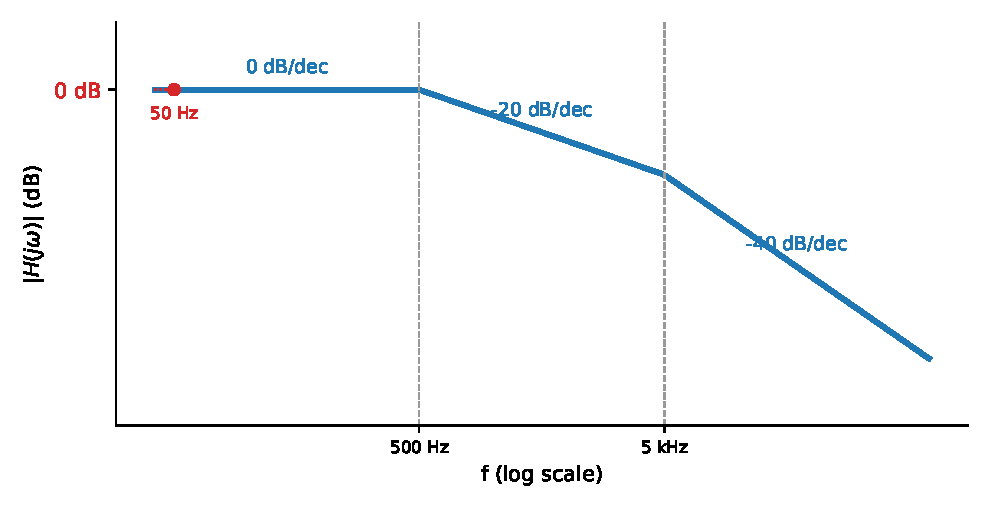
\includegraphics[width=\linewidth,height=5cm,keepaspectratio]{p12_plot}\end{center}
\solstep{1}{Read the corners and slopes}Go left to right along the plot and write down the slope of every straight segment. At each corner frequency the slope changes by a multiple of 20\,dB/dec: every $-20$ is one pole, every $+20$ is one zero (tool T6 read backwards).\begin{center}\renewcommand{\arraystretch}{1.35}
\begin{tabular}{ccccl}
\toprule
corner $f_c$ & slope before & slope after & change & meaning \\
\midrule
500 Hz & $0$ & $-20$ & $-20$ & one pole at $f_c$ \\
5 kHz & $-20$ & $-40$ & $-20$ & one pole at $f_c$ \\
\bottomrule
\end{tabular}\end{center}

\solstep{2}{Starting slope $\Rightarrow$ factors of $s$}The plot starts \emph{flat} (0\,dB/dec), so there is no factor $s$ in the numerator: every pole is written as $\frac{1}{1+s/p}$ and every zero as $\left(1+\frac{s}{z}\right)$, which are all $\approx1$ (0\,dB) at low frequency. Every corner is an angular frequency $\omega_c=2\pi f_c$.
\solstep{3}{Assemble $H(s)$}Put one factor per pole/zero in front of an unknown constant $K$:\[
H(s) = K\,\dfrac{1}{1+\dfrac{s}{2\pi\cdot 500}}\,\dfrac{1}{1+\dfrac{s}{2\pi\cdot 5\mathrm{k}}}
\]

\solstep{4}{Find $K$ from the marked level}The plot marks the level $0$\,dB at $f=$\,50 Hz. On the straight-line plot every factor is either exactly 0\,dB (where it is $\approx1$) or a $\pm20$\,dB/dec line, so evaluate the \emph{asymptote} of each factor at that frequency (the level of a line with slope $\pm20$\,dB/dec is $\pm20\log_{10}(f/f_c)$):\begin{center}\renewcommand{\arraystretch}{1.35}
\begin{tabular}{cccc}
\toprule
factor & $f_c$ & at $f=$\,50 Hz & asymptote (dB) \\
\midrule
$\rule[-1.7em]{0pt}{4em}\dfrac{1}{1+\dfrac{s}{2\pi\cdot 500}}$ & 500 Hz & $f<f_c$: $\approx 1$ & $0$ \\
$\rule[-1.7em]{0pt}{4em}\dfrac{1}{1+\dfrac{s}{2\pi\cdot 5\mathrm{k}}}$ & 5 kHz & $f<f_c$: $\approx 1$ & $0$ \\
\textbf{sum} &  &  & $\mathbf{0}$ \\
\bottomrule
\end{tabular}\end{center}
The dB values of the factors \emph{add} (magnitudes multiply), so\[
20\log_{10}K = 0 - (0) = 0\ \mathrm{dB}\quad\Rightarrow\quad K = 10^{0/20} = 1
\]

So\[
\boxed{H(s) = 1\,\dfrac{1}{1+\dfrac{s}{2\pi\cdot 500}}\,\dfrac{1}{1+\dfrac{s}{2\pi\cdot 5\mathrm{k}}}}
\]


\solstep{5}{Split $H(s)$ into op-amp stages}Every inverting stage of the form $-\frac{Z_f}{Z_{in}}$ with $Z_{in}$, $Z_f$ made of one R and at most one C realizes \emph{one} pole, optionally with one zero or one $s$ (tool T2). Pair each zero with a low-pass pole (pole-zero stage), each $\frac{s}{s+p}$ with a remaining low-pass pole (band-pass stage), and give every leftover factor its own stage. Put all of $|K|$ into the first stage. Each stage inverts, so with an odd number of stages add a unity-gain inverter to make $K>0$.\begin{center}\renewcommand{\arraystretch}{1.35}
\begin{tabular}{cccl}
\toprule
stage & gain $\frac{R_2}{R_1}$ & factor(s) realized & block \\
\midrule
U1 & $1$ & $\rule[-1.4em]{0pt}{3.4em}\dfrac{1}{1+\frac{s}{2\pi\cdot 500}}$ & low-pass: $Z_{in}=R$, $Z_f=R\parallel C$ \\
U2 & $1$ & $\rule[-1.4em]{0pt}{3.4em}\dfrac{1}{1+\frac{s}{2\pi\cdot 5\mathrm{k}}}$ & low-pass: $Z_{in}=R$, $Z_f=R\parallel C$ \\
\bottomrule
\end{tabular}\end{center}

\solstep{6}{Component values}Use $R_1 = 10\,\mathrm{k}\Omega$ at the input of every stage (any convenient value works; it only scales the other parts). The corner of a factor $1+s/\omega_c$ is matched by $RC = 1/\omega_c$ (corners in rad/s).\begin{enumerate}[leftmargin=*,itemsep=2pt]
\item U1: choose $R_{1} = 10\,\mathrm{k}\Omega$, then match the stage formula $-\frac{R_{2}}{R_{1}}\cdot\frac{1}{1+sR_{2}C_{1}}$ to the factors:\[
R_{2} = 1\,R_{1} = 10\,\mathrm{k}\Omega,\qquad C_{1} = \frac{1}{3140\,R_{2}} = 31.8\,\mathrm{n}\mathrm{F}
\]

\item U2: choose $R_{3} = 10\,\mathrm{k}\Omega$, then match the stage formula $-\frac{R_{4}}{R_{3}}\cdot\frac{1}{1+sR_{4}C_{2}}$ to the factors:\[
R_{4} = 1\,R_{3} = 10\,\mathrm{k}\Omega,\qquad C_{2} = \frac{1}{31400\,R_{4}} = 3.18\,\mathrm{n}\mathrm{F}
\]

\end{enumerate}

\solstep{7}{Check and steady-state output}The designed circuit:\begin{center}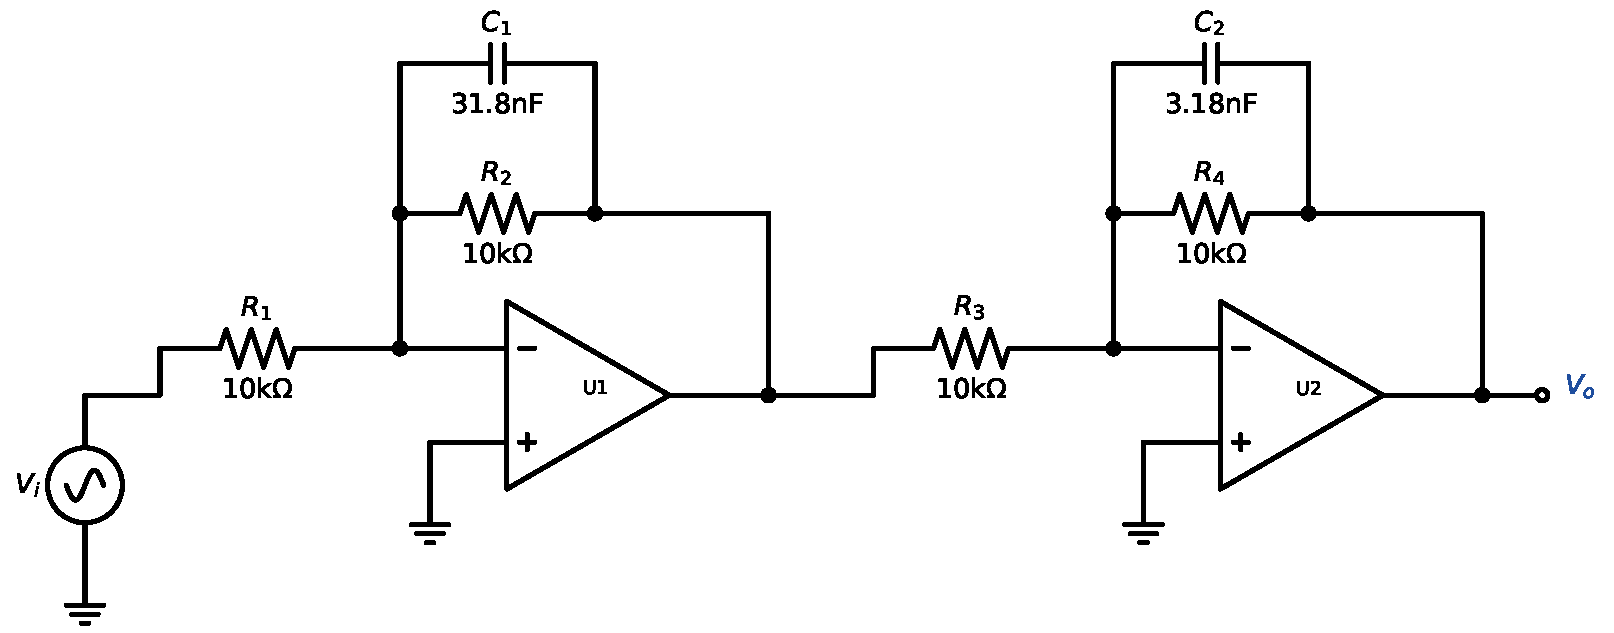
\includegraphics[width=\linewidth,height=5.5cm,keepaspectratio]{p12_design}\end{center}
Check: the stage gains multiply to $(-1)^{2}\cdot1\cdot(\text{factors}) = H(s)$; an independent nodal solve of this circuit reproduces $H(s)$ at every frequency. (Standard-value resistors and capacitors would move the corners slightly.)

The input is $V_i(t) = 1\sin\left(2\pi\cdot 1000\,t+\frac{\pi}{4}\right)$, so $\omega_{in} = 2\pi\cdot 1000 = 6280$\,rad/s. Put $s=j\omega_{in}$ in each factor (tool T5): magnitudes multiply, angles add.
{\small Rules: $\left|\frac{s}{s+p}\right| = \frac{\omega}{\sqrt{\omega^2+p^2}}$, $\angle = \frac{\pi}{2}-\tan^{-1}\frac{\omega}{p}$;\quad $\left|\frac{1}{1+s/p}\right| = \frac{1}{\sqrt{1+(\omega/p)^2}}$, $\angle = -\tan^{-1}\frac{\omega}{p}$;\quad $\left|1+\frac{s}{z}\right| = \sqrt{1+(\omega/z)^2}$, $\angle = \tan^{-1}\frac{\omega}{z}$;\quad a negative $K$ adds $-\pi$.}
\begin{center}\renewcommand{\arraystretch}{1.35}
\begin{tabular}{ccc}
\toprule
factor & magnitude & angle (rad) \\
\midrule
$1$ & $1$ & $0$ \\
$\rule[-1.7em]{0pt}{4em}\dfrac{1}{1+\dfrac{s}{2\pi\cdot 500}}$ & $0.4472$ & $-1.11$ \\
$\rule[-1.7em]{0pt}{4em}\dfrac{1}{1+\dfrac{s}{2\pi\cdot 5\mathrm{k}}}$ & $0.9806$ & $-0.197$ \\
\textbf{total} & $\mathbf{0.4385}$ (product) & $\mathbf{-1.3}$ (sum) \\
\bottomrule
\end{tabular}\end{center}

\begin{align*}
|H(j\omega_{in})| &= 0.439, \qquad \angle H(j\omega_{in}) = -1.3\ \mathrm{rad} \\
v_{o,ac}(t) &= 0.439\times 1\,\sin\left(2\pi\cdot 1000\,t - 0.519\right) = 0.439\,\sin\left(2\pi\cdot 1000\,t - 0.519\right)
\end{align*}

(phase: $\theta + \angle H = \frac{\pi}{4} + (-1.3) = -0.519$\,rad.)
\[
\boxed{V_o(t) = 0.439\,\sin\left(2\pi\cdot 1000\,t - 0.519\right)\ \mathrm{V}}
\]

\begin{ansbox}
$H(s) = 1\,\dfrac{1}{1+\dfrac{s}{2\pi\cdot 500}}\,\dfrac{1}{1+\dfrac{s}{2\pi\cdot 5\mathrm{k}}}$\\[4pt]
U1: R1 = 10k$\Omega$, R2 = 10k$\Omega$, C1 = 31.8nF\\
U2: R3 = 10k$\Omega$, R4 = 10k$\Omega$, C2 = 3.18nF\\[4pt]
$V_o(t) = 0.439\,\sin\left(2\pi\cdot 1000\,t - 0.519\right)\ \mathrm{V}$
\end{ansbox}

\newpage
\subsection*{Solution 2C.13 \hfill Hard}
\begin{center}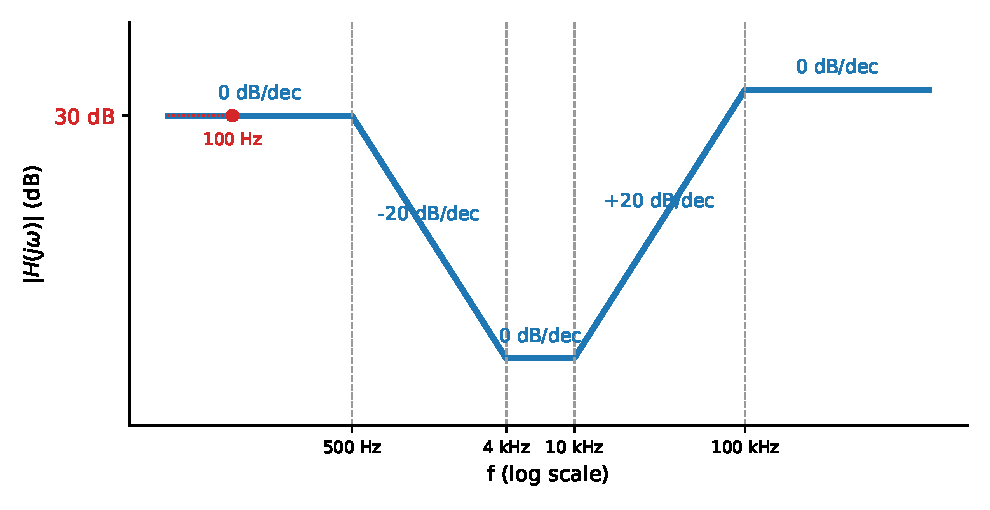
\includegraphics[width=\linewidth,height=5cm,keepaspectratio]{p13_plot}\end{center}
\solstep{1}{Read the corners and slopes}Go left to right along the plot and write down the slope of every straight segment. At each corner frequency the slope changes by a multiple of 20\,dB/dec: every $-20$ is one pole, every $+20$ is one zero (tool T6 read backwards).\begin{center}\renewcommand{\arraystretch}{1.35}
\begin{tabular}{ccccl}
\toprule
corner $f_c$ & slope before & slope after & change & meaning \\
\midrule
500 Hz & $0$ & $-20$ & $-20$ & one pole at $f_c$ \\
4 kHz & $-20$ & $0$ & $+20$ & one zero at $f_c$ \\
10 kHz & $0$ & $+20$ & $+20$ & one zero at $f_c$ \\
100 kHz & $+20$ & $0$ & $-20$ & one pole at $f_c$ \\
\bottomrule
\end{tabular}\end{center}

\solstep{2}{Starting slope $\Rightarrow$ factors of $s$}The plot starts \emph{flat} (0\,dB/dec), so there is no factor $s$ in the numerator: every pole is written as $\frac{1}{1+s/p}$ and every zero as $\left(1+\frac{s}{z}\right)$, which are all $\approx1$ (0\,dB) at low frequency. Every corner is an angular frequency $\omega_c=2\pi f_c$.
\solstep{3}{Assemble $H(s)$}Put one factor per pole/zero in front of an unknown constant $K$:\[
H(s) = K\,\dfrac{1}{1+\dfrac{s}{2\pi\cdot 500}}\,\left(1+\dfrac{s}{2\pi\cdot 4\mathrm{k}}\right)\,\left(1+\dfrac{s}{2\pi\cdot 10\mathrm{k}}\right)\,\dfrac{1}{1+\dfrac{s}{2\pi\cdot 100\mathrm{k}}}
\]

\solstep{4}{Find $K$ from the marked level}The plot marks the level $30$\,dB at $f=$\,100 Hz. On the straight-line plot every factor is either exactly 0\,dB (where it is $\approx1$) or a $\pm20$\,dB/dec line, so evaluate the \emph{asymptote} of each factor at that frequency (the level of a line with slope $\pm20$\,dB/dec is $\pm20\log_{10}(f/f_c)$):\begin{center}\renewcommand{\arraystretch}{1.35}
\begin{tabular}{cccc}
\toprule
factor & $f_c$ & at $f=$\,100 Hz & asymptote (dB) \\
\midrule
$\rule[-1.7em]{0pt}{4em}\dfrac{1}{1+\dfrac{s}{2\pi\cdot 500}}$ & 500 Hz & $f<f_c$: $\approx 1$ & $0$ \\
$\rule[-1.1em]{0pt}{2.8em}\left(1+\dfrac{s}{2\pi\cdot 4\mathrm{k}}\right)$ & 4 kHz & $f<f_c$: $\approx 1$ & $0$ \\
$\rule[-1.1em]{0pt}{2.8em}\left(1+\dfrac{s}{2\pi\cdot 10\mathrm{k}}\right)$ & 10 kHz & $f<f_c$: $\approx 1$ & $0$ \\
$\rule[-1.7em]{0pt}{4em}\dfrac{1}{1+\dfrac{s}{2\pi\cdot 100\mathrm{k}}}$ & 100 kHz & $f<f_c$: $\approx 1$ & $0$ \\
\textbf{sum} &  &  & $\mathbf{0}$ \\
\bottomrule
\end{tabular}\end{center}
The dB values of the factors \emph{add} (magnitudes multiply), so\[
20\log_{10}K = 30 - (0) = 30\ \mathrm{dB}\quad\Rightarrow\quad K = 10^{30/20} = 31.6
\]

So\[
\boxed{H(s) = 31.6\,\dfrac{1}{1+\dfrac{s}{2\pi\cdot 500}}\,\left(1+\dfrac{s}{2\pi\cdot 4\mathrm{k}}\right)\,\left(1+\dfrac{s}{2\pi\cdot 10\mathrm{k}}\right)\,\dfrac{1}{1+\dfrac{s}{2\pi\cdot 100\mathrm{k}}}}
\]


\solstep{5}{Split $H(s)$ into op-amp stages}Every inverting stage of the form $-\frac{Z_f}{Z_{in}}$ with $Z_{in}$, $Z_f$ made of one R and at most one C realizes \emph{one} pole, optionally with one zero or one $s$ (tool T2). Pair each zero with a low-pass pole (pole-zero stage), each $\frac{s}{s+p}$ with a remaining low-pass pole (band-pass stage), and give every leftover factor its own stage. Put all of $|K|$ into the first stage. Each stage inverts, so with an odd number of stages add a unity-gain inverter to make $K>0$.\begin{center}\renewcommand{\arraystretch}{1.35}
\begin{tabular}{cccl}
\toprule
stage & gain $\frac{R_2}{R_1}$ & factor(s) realized & block \\
\midrule
U1 & $31.62$ & $\rule[-1.4em]{0pt}{3.4em}\dfrac{1+\frac{s}{2\pi\cdot 4\mathrm{k}}}{1+\frac{s}{2\pi\cdot 500}}$ & pole-zero: $Z_{in}=R\parallel C$, $Z_f = R\parallel C$ \\
U2 & $1$ & $\rule[-1.4em]{0pt}{3.4em}\dfrac{1+\frac{s}{2\pi\cdot 10\mathrm{k}}}{1+\frac{s}{2\pi\cdot 100\mathrm{k}}}$ & pole-zero: $Z_{in}=R\parallel C$, $Z_f = R\parallel C$ \\
\bottomrule
\end{tabular}\end{center}

\solstep{6}{Component values}Use $R_1 = 10\,\mathrm{k}\Omega$ at the input of every stage (any convenient value works; it only scales the other parts). The corner of a factor $1+s/\omega_c$ is matched by $RC = 1/\omega_c$ (corners in rad/s).\begin{enumerate}[leftmargin=*,itemsep=2pt]
\item U1: choose $R_{1} = 10\,\mathrm{k}\Omega$, then match the stage formula $-\frac{R_{2}}{R_{1}}\cdot\frac{1+sR_{1}C_{1}}{1+sR_{2}C_{2}}$ to the factors:\[
R_{2} = 31.62\,R_{1} = 316\,\mathrm{k}\Omega,\qquad C_{1} = \frac{1}{25100\,R_{1}} = 3.98\,\mathrm{n}\mathrm{F},\qquad C_{2} = \frac{1}{3140\,R_{2}} = 1.01\,\mathrm{n}\mathrm{F}
\]

\item U2: choose $R_{3} = 10\,\mathrm{k}\Omega$, then match the stage formula $-\frac{R_{4}}{R_{3}}\cdot\frac{1+sR_{3}C_{3}}{1+sR_{4}C_{4}}$ to the factors:\[
R_{4} = 1\,R_{3} = 10\,\mathrm{k}\Omega,\qquad C_{3} = \frac{1}{62800\,R_{3}} = 1.59\,\mathrm{n}\mathrm{F},\qquad C_{4} = \frac{1}{6.28\times 10^{5}\,R_{4}} = 159\,\mathrm{p}\mathrm{F}
\]

\end{enumerate}

\solstep{7}{Check and steady-state output}The designed circuit:\begin{center}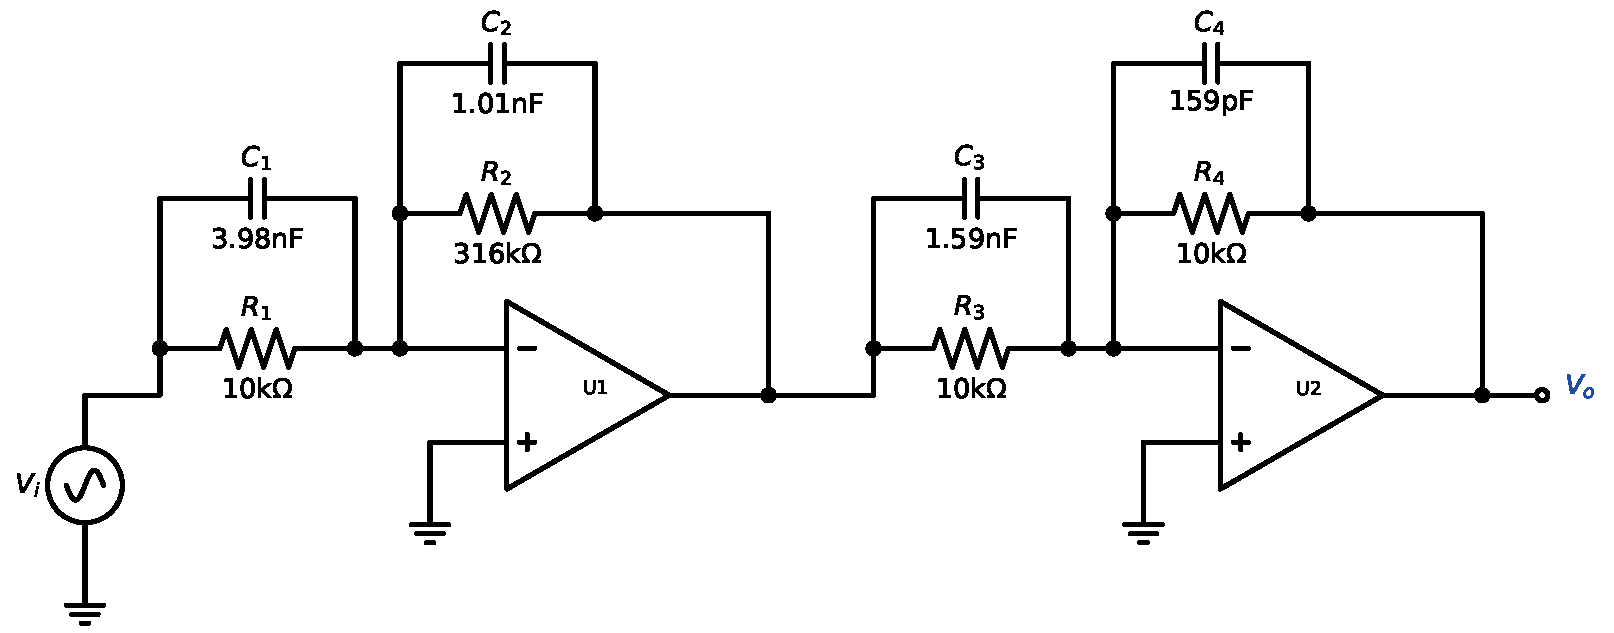
\includegraphics[width=\linewidth,height=5.5cm,keepaspectratio]{p13_design}\end{center}
Check: the stage gains multiply to $(-1)^{2}\cdot31.62\cdot(\text{factors}) = H(s)$; an independent nodal solve of this circuit reproduces $H(s)$ at every frequency. (Standard-value resistors and capacitors would move the corners slightly.)

The input is $V_i(t) = 0.01\sin\left(2\pi\cdot 2000\,t\right)$, so $\omega_{in} = 2\pi\cdot 2000 = 12600$\,rad/s. Put $s=j\omega_{in}$ in each factor (tool T5): magnitudes multiply, angles add.
{\small Rules: $\left|\frac{s}{s+p}\right| = \frac{\omega}{\sqrt{\omega^2+p^2}}$, $\angle = \frac{\pi}{2}-\tan^{-1}\frac{\omega}{p}$;\quad $\left|\frac{1}{1+s/p}\right| = \frac{1}{\sqrt{1+(\omega/p)^2}}$, $\angle = -\tan^{-1}\frac{\omega}{p}$;\quad $\left|1+\frac{s}{z}\right| = \sqrt{1+(\omega/z)^2}$, $\angle = \tan^{-1}\frac{\omega}{z}$;\quad a negative $K$ adds $-\pi$.}
\begin{center}\renewcommand{\arraystretch}{1.35}
\begin{tabular}{ccc}
\toprule
factor & magnitude & angle (rad) \\
\midrule
$31.6$ & $31.62$ & $0$ \\
$\rule[-1.7em]{0pt}{4em}\dfrac{1}{1+\dfrac{s}{2\pi\cdot 500}}$ & $0.2425$ & $-1.33$ \\
$\rule[-1.1em]{0pt}{2.8em}\left(1+\dfrac{s}{2\pi\cdot 4\mathrm{k}}\right)$ & $1.118$ & $0.464$ \\
$\rule[-1.1em]{0pt}{2.8em}\left(1+\dfrac{s}{2\pi\cdot 10\mathrm{k}}\right)$ & $1.02$ & $0.197$ \\
$\rule[-1.7em]{0pt}{4em}\dfrac{1}{1+\dfrac{s}{2\pi\cdot 100\mathrm{k}}}$ & $0.9998$ & $-0.02$ \\
\textbf{total} & $\mathbf{8.743}$ (product) & $\mathbf{-0.685}$ (sum) \\
\bottomrule
\end{tabular}\end{center}

\begin{align*}
|H(j\omega_{in})| &= 8.74, \qquad \angle H(j\omega_{in}) = -0.685\ \mathrm{rad} \\
v_{o,ac}(t) &= 8.74\times 0.01\,\sin\left(2\pi\cdot 2000\,t - 0.685\right) = 0.0874\,\sin\left(2\pi\cdot 2000\,t - 0.685\right)
\end{align*}

\[
\boxed{V_o(t) = 0.0874\,\sin\left(2\pi\cdot 2000\,t - 0.685\right)\ \mathrm{V}}
\]

\begin{ansbox}
$H(s) = 31.6\,\dfrac{1}{1+\dfrac{s}{2\pi\cdot 500}}\,\left(1+\dfrac{s}{2\pi\cdot 4\mathrm{k}}\right)\,\left(1+\dfrac{s}{2\pi\cdot 10\mathrm{k}}\right)\,\dfrac{1}{1+\dfrac{s}{2\pi\cdot 100\mathrm{k}}}$\\[4pt]
U1: R1 = 10k$\Omega$, C1 = 3.98nF, R2 = 316k$\Omega$, C2 = 1.01nF\\
U2: R3 = 10k$\Omega$, C3 = 1.59nF, R4 = 10k$\Omega$, C4 = 159pF\\[4pt]
$V_o(t) = 0.0874\,\sin\left(2\pi\cdot 2000\,t - 0.685\right)\ \mathrm{V}$
\end{ansbox}

\newpage
\subsection*{Solution 2C.14 \hfill Hard}
\begin{center}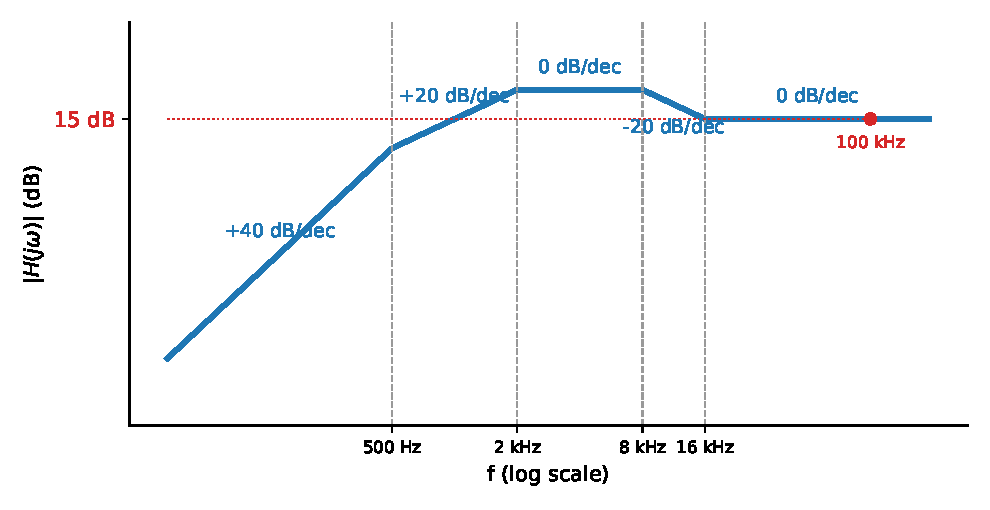
\includegraphics[width=\linewidth,height=5cm,keepaspectratio]{p14_plot}\end{center}
\solstep{1}{Read the corners and slopes}Go left to right along the plot and write down the slope of every straight segment. At each corner frequency the slope changes by a multiple of 20\,dB/dec: every $-20$ is one pole, every $+20$ is one zero (tool T6 read backwards).\begin{center}\renewcommand{\arraystretch}{1.35}
\begin{tabular}{ccccl}
\toprule
corner $f_c$ & slope before & slope after & change & meaning \\
\midrule
500 Hz & $+40$ & $+20$ & $-20$ & one pole at $f_c$ \\
2 kHz & $+20$ & $0$ & $-20$ & one pole at $f_c$ \\
8 kHz & $0$ & $-20$ & $-20$ & one pole at $f_c$ \\
16 kHz & $-20$ & $0$ & $+20$ & one zero at $f_c$ \\
\bottomrule
\end{tabular}\end{center}

\solstep{2}{Starting slope $\Rightarrow$ factors of $s$}The plot starts with a slope of $+40$\,dB/dec, i.e. $|H|\propto\omega^2$ at low frequency: the numerator contains $s^2$. As in class, pair each $s$ with one of the \emph{lowest} poles (500 Hz, 2 kHz) as $\frac{s}{s+p}$: such a factor rises at $+20$\,dB/dec below $p$ and is $\approx1$ (0\,dB) above it. The remaining poles are written $\frac{1}{1+s/p}$ and the zeros $\left(1+\frac{s}{z}\right)$. Every corner is an angular frequency $\omega_c=2\pi f_c$.
\solstep{3}{Assemble $H(s)$}Put one factor per pole/zero in front of an unknown constant $K$:\[
H(s) = K\,\dfrac{s}{s+2\pi\cdot 500}\,\dfrac{s}{s+2\pi\cdot 2\mathrm{k}}\,\dfrac{1}{1+\dfrac{s}{2\pi\cdot 8\mathrm{k}}}\,\left(1+\dfrac{s}{2\pi\cdot 16\mathrm{k}}\right)
\]

\solstep{4}{Find $K$ from the marked level}The plot marks the level $15$\,dB at $f=$\,100 kHz. On the straight-line plot every factor is either exactly 0\,dB (where it is $\approx1$) or a $\pm20$\,dB/dec line, so evaluate the \emph{asymptote} of each factor at that frequency (the level of a line with slope $\pm20$\,dB/dec is $\pm20\log_{10}(f/f_c)$):\begin{center}\renewcommand{\arraystretch}{1.35}
\begin{tabular}{cccc}
\toprule
factor & $f_c$ & at $f=$\,100 kHz & asymptote (dB) \\
\midrule
$\rule[-1.1em]{0pt}{2.8em}\dfrac{s}{s+2\pi\cdot 500}$ & 500 Hz & $f>f_c$: $\approx 1$ & $0$ \\
$\rule[-1.1em]{0pt}{2.8em}\dfrac{s}{s+2\pi\cdot 2\mathrm{k}}$ & 2 kHz & $f>f_c$: $\approx 1$ & $0$ \\
$\rule[-1.7em]{0pt}{4em}\dfrac{1}{1+\dfrac{s}{2\pi\cdot 8\mathrm{k}}}$ & 8 kHz & $f>f_c$: $\approx \frac{p}{\omega}$ & $-21.9$ \\
$\rule[-1.1em]{0pt}{2.8em}\left(1+\dfrac{s}{2\pi\cdot 16\mathrm{k}}\right)$ & 16 kHz & $f>f_c$: $\approx \frac{\omega}{z}$ & $15.9$ \\
\textbf{sum} &  &  & $\mathbf{-6.02}$ \\
\bottomrule
\end{tabular}\end{center}
The dB values of the factors \emph{add} (magnitudes multiply), so\[
20\log_{10}K = 15 - (-6.02) = 21\ \mathrm{dB}\quad\Rightarrow\quad K = 10^{21/20} = 11.2
\]

So\[
\boxed{H(s) = 11.2\,\dfrac{s}{s+2\pi\cdot 500}\,\dfrac{s}{s+2\pi\cdot 2\mathrm{k}}\,\dfrac{1}{1+\dfrac{s}{2\pi\cdot 8\mathrm{k}}}\,\left(1+\dfrac{s}{2\pi\cdot 16\mathrm{k}}\right)}
\]


\solstep{5}{Split $H(s)$ into op-amp stages}Every inverting stage of the form $-\frac{Z_f}{Z_{in}}$ with $Z_{in}$, $Z_f$ made of one R and at most one C realizes \emph{one} pole, optionally with one zero or one $s$ (tool T2). Pair each zero with a low-pass pole (pole-zero stage), each $\frac{s}{s+p}$ with a remaining low-pass pole (band-pass stage), and give every leftover factor its own stage. Put all of $|K|$ into the first stage. Each stage inverts, so with an odd number of stages add a unity-gain inverter to make $K>0$.\begin{center}\renewcommand{\arraystretch}{1.35}
\begin{tabular}{cccl}
\toprule
stage & gain $\frac{R_2}{R_1}$ & factor(s) realized & block \\
\midrule
U1 & $11.25$ & $\rule[-1.4em]{0pt}{3.4em}\dfrac{s}{s+2\pi\cdot 500}$ & high-pass: $Z_{in}=R+\frac{1}{sC}$, $Z_f=R$ \\
U2 & $1$ & $\rule[-1.4em]{0pt}{3.4em}\dfrac{s}{s+2\pi\cdot 2\mathrm{k}}$ & high-pass: $Z_{in}=R+\frac{1}{sC}$, $Z_f=R$ \\
U3 & $1$ & $\rule[-1.4em]{0pt}{3.4em}\dfrac{1+\frac{s}{2\pi\cdot 16\mathrm{k}}}{1+\frac{s}{2\pi\cdot 8\mathrm{k}}}$ & pole-zero: $Z_{in}=R\parallel C$, $Z_f = R\parallel C$ \\
U4 & $1$ & $\rule[-1.4em]{0pt}{3.4em}1$ & unity inverter (fixes the sign) \\
\bottomrule
\end{tabular}\end{center}

\solstep{6}{Component values}Use $R_1 = 10\,\mathrm{k}\Omega$ at the input of every stage (any convenient value works; it only scales the other parts). The corner of a factor $1+s/\omega_c$ is matched by $RC = 1/\omega_c$ (corners in rad/s).\begin{enumerate}[leftmargin=*,itemsep=2pt]
\item U1: choose $R_{1} = 10\,\mathrm{k}\Omega$, then match the stage formula $-\frac{R_{2}}{R_{1}}\cdot\frac{s}{s+1/(R_{1}C_{1})}$ to the factors:\[
C_{1} = \frac{1}{3140\,R_{1}} = 31.8\,\mathrm{n}\mathrm{F},\qquad R_{2} = 11.25\,R_{1} = 112\,\mathrm{k}\Omega
\]

\item U2: choose $R_{3} = 10\,\mathrm{k}\Omega$, then match the stage formula $-\frac{R_{4}}{R_{3}}\cdot\frac{s}{s+1/(R_{3}C_{2})}$ to the factors:\[
C_{2} = \frac{1}{12600\,R_{3}} = 7.96\,\mathrm{n}\mathrm{F},\qquad R_{4} = 1\,R_{3} = 10\,\mathrm{k}\Omega
\]

\item U3: choose $R_{5} = 10\,\mathrm{k}\Omega$, then match the stage formula $-\frac{R_{6}}{R_{5}}\cdot\frac{1+sR_{5}C_{3}}{1+sR_{6}C_{4}}$ to the factors:\[
R_{6} = 1\,R_{5} = 10\,\mathrm{k}\Omega,\qquad C_{3} = \frac{1}{1.01\times 10^{5}\,R_{5}} = 995\,\mathrm{p}\mathrm{F},\qquad C_{4} = \frac{1}{50300\,R_{6}} = 1.99\,\mathrm{n}\mathrm{F}
\]

\item U4: $R_{7} = R_{8} = 10\,\mathrm{k}\Omega$ (gain $-1$).
\end{enumerate}

\solstep{7}{Check and steady-state output}The designed circuit:\begin{center}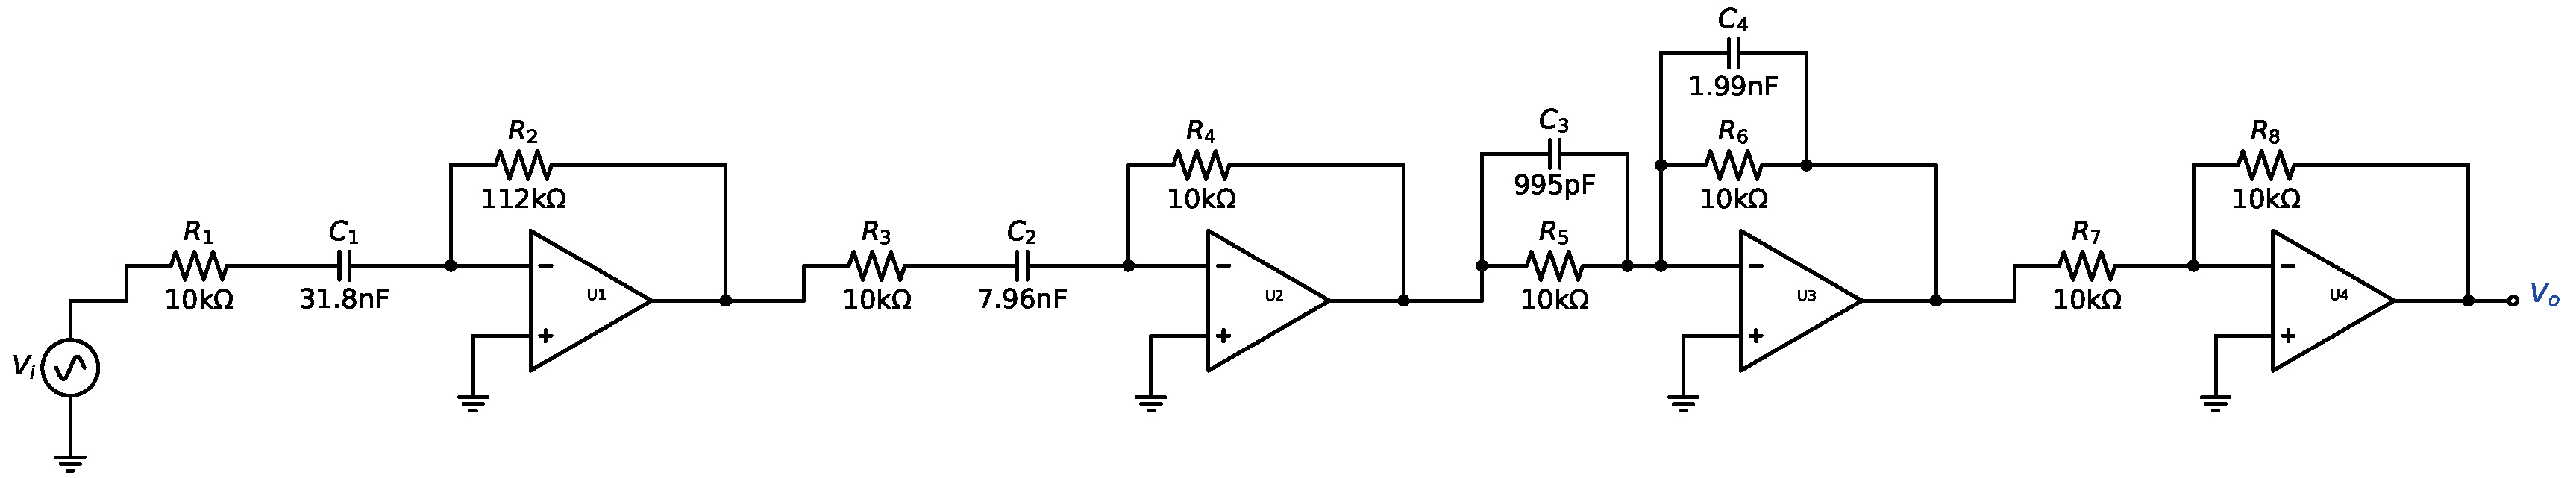
\includegraphics[width=\linewidth,height=5.5cm,keepaspectratio]{p14_design}\end{center}
Check: the stage gains multiply to $(-1)^{4}\cdot11.25\cdot(\text{factors}) = H(s)$; an independent nodal solve of this circuit reproduces $H(s)$ at every frequency. (Standard-value resistors and capacitors would move the corners slightly.)

The input is $V_i(t) = 0.3\sin\left(2\pi\cdot 10000\,t\right)$, so $\omega_{in} = 2\pi\cdot 10000 = 62800$\,rad/s. Put $s=j\omega_{in}$ in each factor (tool T5): magnitudes multiply, angles add.
{\small Rules: $\left|\frac{s}{s+p}\right| = \frac{\omega}{\sqrt{\omega^2+p^2}}$, $\angle = \frac{\pi}{2}-\tan^{-1}\frac{\omega}{p}$;\quad $\left|\frac{1}{1+s/p}\right| = \frac{1}{\sqrt{1+(\omega/p)^2}}$, $\angle = -\tan^{-1}\frac{\omega}{p}$;\quad $\left|1+\frac{s}{z}\right| = \sqrt{1+(\omega/z)^2}$, $\angle = \tan^{-1}\frac{\omega}{z}$;\quad a negative $K$ adds $-\pi$.}
\begin{center}\renewcommand{\arraystretch}{1.35}
\begin{tabular}{ccc}
\toprule
factor & magnitude & angle (rad) \\
\midrule
$11.2$ & $11.25$ & $0$ \\
$\rule[-1.1em]{0pt}{2.8em}\dfrac{s}{s+2\pi\cdot 500}$ & $0.9988$ & $0.05$ \\
$\rule[-1.1em]{0pt}{2.8em}\dfrac{s}{s+2\pi\cdot 2\mathrm{k}}$ & $0.9806$ & $0.197$ \\
$\rule[-1.7em]{0pt}{4em}\dfrac{1}{1+\dfrac{s}{2\pi\cdot 8\mathrm{k}}}$ & $0.6247$ & $-0.896$ \\
$\rule[-1.1em]{0pt}{2.8em}\left(1+\dfrac{s}{2\pi\cdot 16\mathrm{k}}\right)$ & $1.179$ & $0.559$ \\
\textbf{total} & $\mathbf{8.114}$ (product) & $\mathbf{-0.0901}$ (sum) \\
\bottomrule
\end{tabular}\end{center}

\begin{align*}
|H(j\omega_{in})| &= 8.11, \qquad \angle H(j\omega_{in}) = -0.0901\ \mathrm{rad} \\
v_{o,ac}(t) &= 8.11\times 0.3\,\sin\left(2\pi\cdot 10000\,t - 0.0901\right) = 2.43\,\sin\left(2\pi\cdot 10000\,t - 0.0901\right)
\end{align*}

\[
\boxed{V_o(t) = 2.43\,\sin\left(2\pi\cdot 10000\,t - 0.0901\right)\ \mathrm{V}}
\]

\begin{ansbox}
$H(s) = 11.2\,\dfrac{s}{s+2\pi\cdot 500}\,\dfrac{s}{s+2\pi\cdot 2\mathrm{k}}\,\dfrac{1}{1+\dfrac{s}{2\pi\cdot 8\mathrm{k}}}\,\left(1+\dfrac{s}{2\pi\cdot 16\mathrm{k}}\right)$\\[4pt]
U1: R1 = 10k$\Omega$, C1 = 31.8nF, R2 = 112k$\Omega$\\
U2: R3 = 10k$\Omega$, C2 = 7.96nF, R4 = 10k$\Omega$\\
U3: R5 = 10k$\Omega$, C3 = 995pF, R6 = 10k$\Omega$, C4 = 1.99nF\\
U4: R7 = 10k$\Omega$, R8 = 10k$\Omega$\\[4pt]
$V_o(t) = 2.43\,\sin\left(2\pi\cdot 10000\,t - 0.0901\right)\ \mathrm{V}$
\end{ansbox}

\newpage
\subsection*{Solution 2C.15 \hfill Hard}
\begin{center}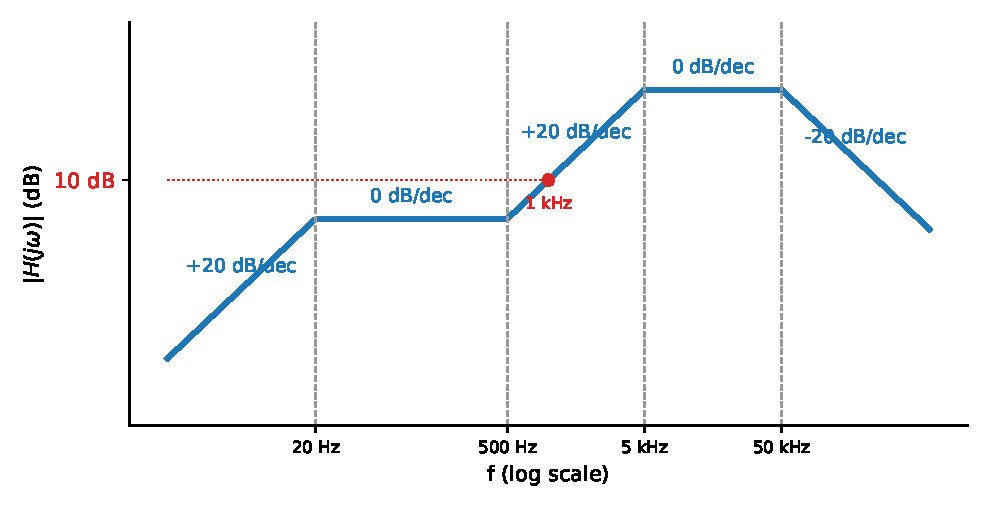
\includegraphics[width=\linewidth,height=5cm,keepaspectratio]{p15_plot}\end{center}
\solstep{1}{Read the corners and slopes}Go left to right along the plot and write down the slope of every straight segment. At each corner frequency the slope changes by a multiple of 20\,dB/dec: every $-20$ is one pole, every $+20$ is one zero (tool T6 read backwards).\begin{center}\renewcommand{\arraystretch}{1.35}
\begin{tabular}{ccccl}
\toprule
corner $f_c$ & slope before & slope after & change & meaning \\
\midrule
20 Hz & $+20$ & $0$ & $-20$ & one pole at $f_c$ \\
500 Hz & $0$ & $+20$ & $+20$ & one zero at $f_c$ \\
5 kHz & $+20$ & $0$ & $-20$ & one pole at $f_c$ \\
50 kHz & $0$ & $-20$ & $-20$ & one pole at $f_c$ \\
\bottomrule
\end{tabular}\end{center}

\solstep{2}{Starting slope $\Rightarrow$ factors of $s$}The plot starts with a slope of $+20$\,dB/dec, i.e. $|H|\propto\omega^1$ at low frequency: the numerator contains $s$. As in class, pair each $s$ with one of the \emph{lowest} poles (20 Hz) as $\frac{s}{s+p}$: such a factor rises at $+20$\,dB/dec below $p$ and is $\approx1$ (0\,dB) above it. The remaining poles are written $\frac{1}{1+s/p}$ and the zeros $\left(1+\frac{s}{z}\right)$. Every corner is an angular frequency $\omega_c=2\pi f_c$.
\solstep{3}{Assemble $H(s)$}Put one factor per pole/zero in front of an unknown constant $K$:\[
H(s) = K\,\dfrac{s}{s+2\pi\cdot 20}\,\left(1+\dfrac{s}{2\pi\cdot 500}\right)\,\dfrac{1}{1+\dfrac{s}{2\pi\cdot 5\mathrm{k}}}\,\dfrac{1}{1+\dfrac{s}{2\pi\cdot 50\mathrm{k}}}
\]

\solstep{4}{Find $K$ from the marked level}The plot marks the level $10$\,dB at $f=$\,1 kHz. On the straight-line plot every factor is either exactly 0\,dB (where it is $\approx1$) or a $\pm20$\,dB/dec line, so evaluate the \emph{asymptote} of each factor at that frequency (the level of a line with slope $\pm20$\,dB/dec is $\pm20\log_{10}(f/f_c)$):\begin{center}\renewcommand{\arraystretch}{1.35}
\begin{tabular}{cccc}
\toprule
factor & $f_c$ & at $f=$\,1 kHz & asymptote (dB) \\
\midrule
$\rule[-1.1em]{0pt}{2.8em}\dfrac{s}{s+2\pi\cdot 20}$ & 20 Hz & $f>f_c$: $\approx 1$ & $0$ \\
$\rule[-1.1em]{0pt}{2.8em}\left(1+\dfrac{s}{2\pi\cdot 500}\right)$ & 500 Hz & $f>f_c$: $\approx \frac{\omega}{z}$ & $6.02$ \\
$\rule[-1.7em]{0pt}{4em}\dfrac{1}{1+\dfrac{s}{2\pi\cdot 5\mathrm{k}}}$ & 5 kHz & $f<f_c$: $\approx 1$ & $0$ \\
$\rule[-1.7em]{0pt}{4em}\dfrac{1}{1+\dfrac{s}{2\pi\cdot 50\mathrm{k}}}$ & 50 kHz & $f<f_c$: $\approx 1$ & $0$ \\
\textbf{sum} &  &  & $\mathbf{6.02}$ \\
\bottomrule
\end{tabular}\end{center}
The dB values of the factors \emph{add} (magnitudes multiply), so\[
20\log_{10}K = 10 - (6.02) = 3.98\ \mathrm{dB}\quad\Rightarrow\quad K = 10^{3.98/20} = 1.58
\]

So\[
\boxed{H(s) = 1.58\,\dfrac{s}{s+2\pi\cdot 20}\,\left(1+\dfrac{s}{2\pi\cdot 500}\right)\,\dfrac{1}{1+\dfrac{s}{2\pi\cdot 5\mathrm{k}}}\,\dfrac{1}{1+\dfrac{s}{2\pi\cdot 50\mathrm{k}}}}
\]


\solstep{5}{Split $H(s)$ into op-amp stages}Every inverting stage of the form $-\frac{Z_f}{Z_{in}}$ with $Z_{in}$, $Z_f$ made of one R and at most one C realizes \emph{one} pole, optionally with one zero or one $s$ (tool T2). Pair each zero with a low-pass pole (pole-zero stage), each $\frac{s}{s+p}$ with a remaining low-pass pole (band-pass stage), and give every leftover factor its own stage. Put all of $|K|$ into the first stage. Each stage inverts, so with an odd number of stages add a unity-gain inverter to make $K>0$.\begin{center}\renewcommand{\arraystretch}{1.35}
\begin{tabular}{cccl}
\toprule
stage & gain $\frac{R_2}{R_1}$ & factor(s) realized & block \\
\midrule
U1 & $1.581$ & $\rule[-1.4em]{0pt}{3.4em}\dfrac{s}{s+2\pi\cdot 20}\cdot\dfrac{1}{1+\frac{s}{2\pi\cdot 50\mathrm{k}}}$ & band-pass: $Z_{in}=R+\frac{1}{sC}$, $Z_f=R\parallel C$ \\
U2 & $1$ & $\rule[-1.4em]{0pt}{3.4em}\dfrac{1+\frac{s}{2\pi\cdot 500}}{1+\frac{s}{2\pi\cdot 5\mathrm{k}}}$ & pole-zero: $Z_{in}=R\parallel C$, $Z_f = R\parallel C$ \\
\bottomrule
\end{tabular}\end{center}

\solstep{6}{Component values}Use $R_1 = 10\,\mathrm{k}\Omega$ at the input of every stage (any convenient value works; it only scales the other parts). The corner of a factor $1+s/\omega_c$ is matched by $RC = 1/\omega_c$ (corners in rad/s).\begin{enumerate}[leftmargin=*,itemsep=2pt]
\item U1: choose $R_{1} = 10\,\mathrm{k}\Omega$, then match the stage formula $-\frac{R_{2}}{R_{1}}\cdot\frac{s}{s+1/(R_{1}C_{1})}\cdot\frac{1}{1+sR_{2}C_{2}}$ to the factors:\[
C_{1} = \frac{1}{126\,R_{1}} = 796\,\mathrm{n}\mathrm{F},\qquad R_{2} = 1.581\,R_{1} = 15.8\,\mathrm{k}\Omega,\qquad C_{2} = \frac{1}{3.14\times 10^{5}\,R_{2}} = 201\,\mathrm{p}\mathrm{F}
\]

\item U2: choose $R_{3} = 10\,\mathrm{k}\Omega$, then match the stage formula $-\frac{R_{4}}{R_{3}}\cdot\frac{1+sR_{3}C_{3}}{1+sR_{4}C_{4}}$ to the factors:\[
R_{4} = 1\,R_{3} = 10\,\mathrm{k}\Omega,\qquad C_{3} = \frac{1}{3140\,R_{3}} = 31.8\,\mathrm{n}\mathrm{F},\qquad C_{4} = \frac{1}{31400\,R_{4}} = 3.18\,\mathrm{n}\mathrm{F}
\]

\end{enumerate}

\solstep{7}{Check and steady-state output}The designed circuit:\begin{center}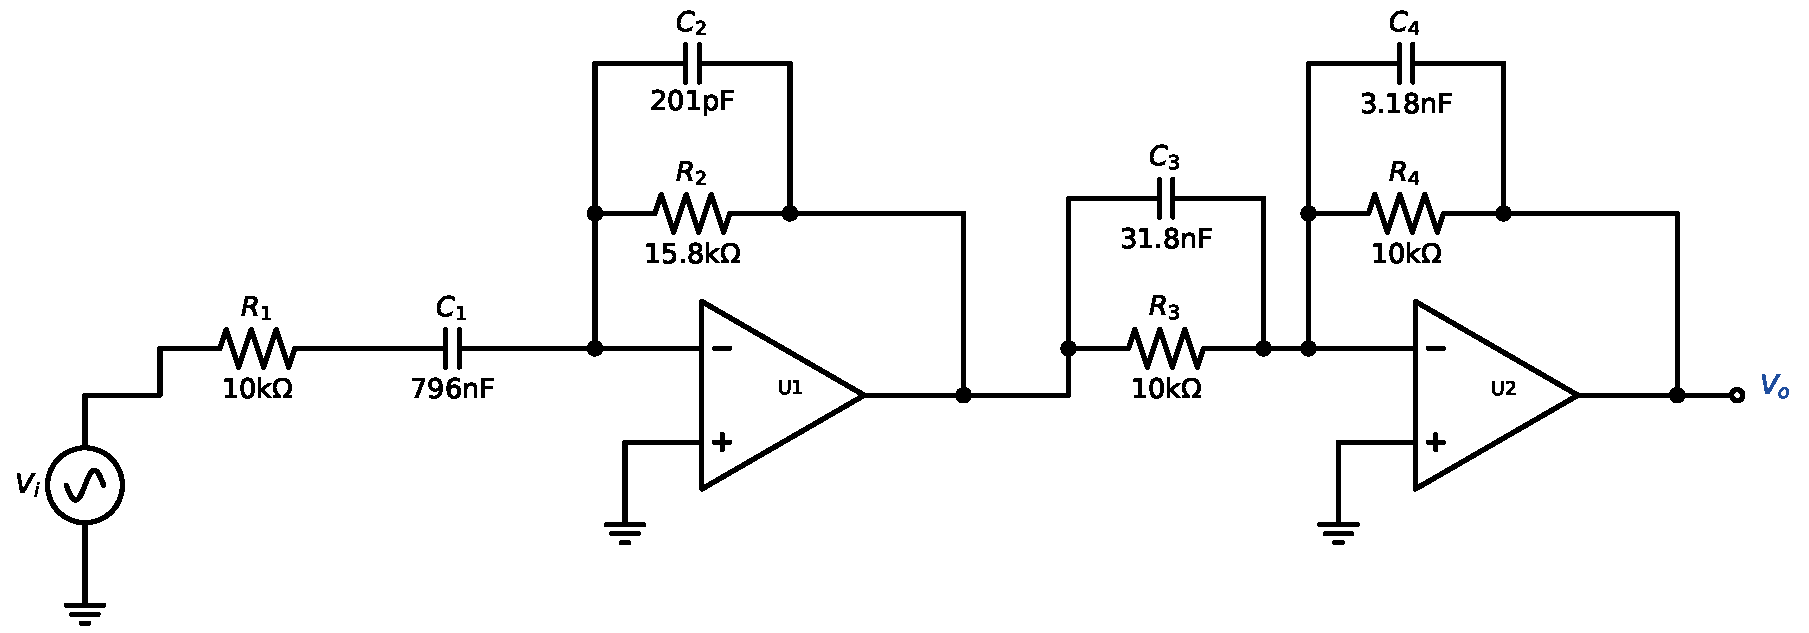
\includegraphics[width=\linewidth,height=5.5cm,keepaspectratio]{p15_design}\end{center}
Check: the stage gains multiply to $(-1)^{2}\cdot1.581\cdot(\text{factors}) = H(s)$; an independent nodal solve of this circuit reproduces $H(s)$ at every frequency. (Standard-value resistors and capacitors would move the corners slightly.)

The input is $V_i(t) = 0.2\sin\left(2\pi\cdot 2000\,t+\frac{\pi}{3}\right)$, so $\omega_{in} = 2\pi\cdot 2000 = 12600$\,rad/s. Put $s=j\omega_{in}$ in each factor (tool T5): magnitudes multiply, angles add.
{\small Rules: $\left|\frac{s}{s+p}\right| = \frac{\omega}{\sqrt{\omega^2+p^2}}$, $\angle = \frac{\pi}{2}-\tan^{-1}\frac{\omega}{p}$;\quad $\left|\frac{1}{1+s/p}\right| = \frac{1}{\sqrt{1+(\omega/p)^2}}$, $\angle = -\tan^{-1}\frac{\omega}{p}$;\quad $\left|1+\frac{s}{z}\right| = \sqrt{1+(\omega/z)^2}$, $\angle = \tan^{-1}\frac{\omega}{z}$;\quad a negative $K$ adds $-\pi$.}
\begin{center}\renewcommand{\arraystretch}{1.35}
\begin{tabular}{ccc}
\toprule
factor & magnitude & angle (rad) \\
\midrule
$1.58$ & $1.581$ & $0$ \\
$\rule[-1.1em]{0pt}{2.8em}\dfrac{s}{s+2\pi\cdot 20}$ & $1$ & $0.01$ \\
$\rule[-1.1em]{0pt}{2.8em}\left(1+\dfrac{s}{2\pi\cdot 500}\right)$ & $4.123$ & $1.33$ \\
$\rule[-1.7em]{0pt}{4em}\dfrac{1}{1+\dfrac{s}{2\pi\cdot 5\mathrm{k}}}$ & $0.9285$ & $-0.381$ \\
$\rule[-1.7em]{0pt}{4em}\dfrac{1}{1+\dfrac{s}{2\pi\cdot 50\mathrm{k}}}$ & $0.9992$ & $-0.04$ \\
\textbf{total} & $\mathbf{6.048}$ (product) & $\mathbf{0.915}$ (sum) \\
\bottomrule
\end{tabular}\end{center}

\begin{align*}
|H(j\omega_{in})| &= 6.05, \qquad \angle H(j\omega_{in}) = 0.915\ \mathrm{rad} \\
v_{o,ac}(t) &= 6.05\times 0.2\,\sin\left(2\pi\cdot 2000\,t + 1.96\right) = 1.21\,\sin\left(2\pi\cdot 2000\,t + 1.96\right)
\end{align*}

(phase: $\theta + \angle H = \frac{\pi}{3} + (0.915) = 1.96$\,rad.)
\[
\boxed{V_o(t) = 1.21\,\sin\left(2\pi\cdot 2000\,t + 1.96\right)\ \mathrm{V}}
\]

\begin{ansbox}
$H(s) = 1.58\,\dfrac{s}{s+2\pi\cdot 20}\,\left(1+\dfrac{s}{2\pi\cdot 500}\right)\,\dfrac{1}{1+\dfrac{s}{2\pi\cdot 5\mathrm{k}}}\,\dfrac{1}{1+\dfrac{s}{2\pi\cdot 50\mathrm{k}}}$\\[4pt]
U1: R1 = 10k$\Omega$, C1 = 796nF, R2 = 15.8k$\Omega$, C2 = 201pF\\
U2: R3 = 10k$\Omega$, C3 = 31.8nF, R4 = 10k$\Omega$, C4 = 3.18nF\\[4pt]
$V_o(t) = 1.21\,\sin\left(2\pi\cdot 2000\,t + 1.96\right)\ \mathrm{V}$
\end{ansbox}

\newpage
\subsection*{Solution 2C.16 \hfill Hard}
\begin{center}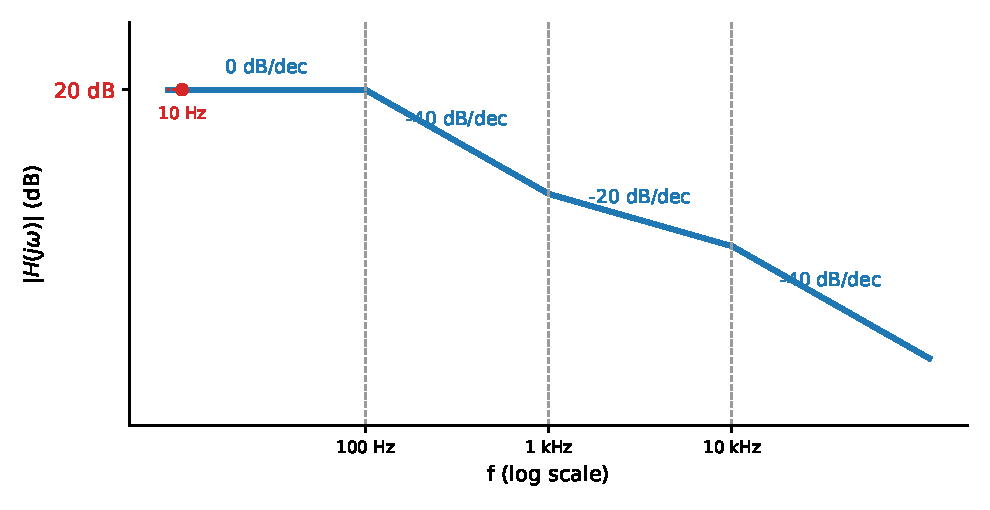
\includegraphics[width=\linewidth,height=5cm,keepaspectratio]{p16_plot}\end{center}
\solstep{1}{Read the corners and slopes}Go left to right along the plot and write down the slope of every straight segment. At each corner frequency the slope changes by a multiple of 20\,dB/dec: every $-20$ is one pole, every $+20$ is one zero (tool T6 read backwards).\begin{center}\renewcommand{\arraystretch}{1.35}
\begin{tabular}{ccccl}
\toprule
corner $f_c$ & slope before & slope after & change & meaning \\
\midrule
100 Hz & $0$ & $-40$ & $-40$ & two poles at $f_c$ \\
1 kHz & $-40$ & $-20$ & $+20$ & one zero at $f_c$ \\
10 kHz & $-20$ & $-40$ & $-20$ & one pole at $f_c$ \\
\bottomrule
\end{tabular}\end{center}

\solstep{2}{Starting slope $\Rightarrow$ factors of $s$}The plot starts \emph{flat} (0\,dB/dec), so there is no factor $s$ in the numerator: every pole is written as $\frac{1}{1+s/p}$ and every zero as $\left(1+\frac{s}{z}\right)$, which are all $\approx1$ (0\,dB) at low frequency. Every corner is an angular frequency $\omega_c=2\pi f_c$.
\solstep{3}{Assemble $H(s)$}Put one factor per pole/zero in front of an unknown constant $K$:\[
H(s) = K\,\dfrac{1}{1+\dfrac{s}{2\pi\cdot 100}}\,\dfrac{1}{1+\dfrac{s}{2\pi\cdot 100}}\,\left(1+\dfrac{s}{2\pi\cdot 1\mathrm{k}}\right)\,\dfrac{1}{1+\dfrac{s}{2\pi\cdot 10\mathrm{k}}}
\]

\solstep{4}{Find $K$ from the marked level}The plot marks the level $20$\,dB at $f=$\,10 Hz. On the straight-line plot every factor is either exactly 0\,dB (where it is $\approx1$) or a $\pm20$\,dB/dec line, so evaluate the \emph{asymptote} of each factor at that frequency (the level of a line with slope $\pm20$\,dB/dec is $\pm20\log_{10}(f/f_c)$):\begin{center}\renewcommand{\arraystretch}{1.35}
\begin{tabular}{cccc}
\toprule
factor & $f_c$ & at $f=$\,10 Hz & asymptote (dB) \\
\midrule
$\rule[-1.7em]{0pt}{4em}\dfrac{1}{1+\dfrac{s}{2\pi\cdot 100}}$ & 100 Hz & $f<f_c$: $\approx 1$ & $0$ \\
$\rule[-1.7em]{0pt}{4em}\dfrac{1}{1+\dfrac{s}{2\pi\cdot 100}}$ & 100 Hz & $f<f_c$: $\approx 1$ & $0$ \\
$\rule[-1.1em]{0pt}{2.8em}\left(1+\dfrac{s}{2\pi\cdot 1\mathrm{k}}\right)$ & 1 kHz & $f<f_c$: $\approx 1$ & $0$ \\
$\rule[-1.7em]{0pt}{4em}\dfrac{1}{1+\dfrac{s}{2\pi\cdot 10\mathrm{k}}}$ & 10 kHz & $f<f_c$: $\approx 1$ & $0$ \\
\textbf{sum} &  &  & $\mathbf{0}$ \\
\bottomrule
\end{tabular}\end{center}
The dB values of the factors \emph{add} (magnitudes multiply), so\[
20\log_{10}K = 20 - (0) = 20\ \mathrm{dB}\quad\Rightarrow\quad K = 10^{20/20} = 10
\]

So\[
\boxed{H(s) = 10\,\dfrac{1}{1+\dfrac{s}{2\pi\cdot 100}}\,\dfrac{1}{1+\dfrac{s}{2\pi\cdot 100}}\,\left(1+\dfrac{s}{2\pi\cdot 1\mathrm{k}}\right)\,\dfrac{1}{1+\dfrac{s}{2\pi\cdot 10\mathrm{k}}}}
\]


\solstep{5}{Split $H(s)$ into op-amp stages}Every inverting stage of the form $-\frac{Z_f}{Z_{in}}$ with $Z_{in}$, $Z_f$ made of one R and at most one C realizes \emph{one} pole, optionally with one zero or one $s$ (tool T2). Pair each zero with a low-pass pole (pole-zero stage), each $\frac{s}{s+p}$ with a remaining low-pass pole (band-pass stage), and give every leftover factor its own stage. Put all of $|K|$ into the first stage. Each stage inverts, so with an odd number of stages add a unity-gain inverter to make $K>0$.\begin{center}\renewcommand{\arraystretch}{1.35}
\begin{tabular}{cccl}
\toprule
stage & gain $\frac{R_2}{R_1}$ & factor(s) realized & block \\
\midrule
U1 & $10$ & $\rule[-1.4em]{0pt}{3.4em}\dfrac{1+\frac{s}{2\pi\cdot 1\mathrm{k}}}{1+\frac{s}{2\pi\cdot 100}}$ & pole-zero: $Z_{in}=R\parallel C$, $Z_f = R\parallel C$ \\
U2 & $1$ & $\rule[-1.4em]{0pt}{3.4em}\dfrac{1}{1+\frac{s}{2\pi\cdot 100}}$ & low-pass: $Z_{in}=R$, $Z_f=R\parallel C$ \\
U3 & $1$ & $\rule[-1.4em]{0pt}{3.4em}\dfrac{1}{1+\frac{s}{2\pi\cdot 10\mathrm{k}}}$ & low-pass: $Z_{in}=R$, $Z_f=R\parallel C$ \\
U4 & $1$ & $\rule[-1.4em]{0pt}{3.4em}1$ & unity inverter (fixes the sign) \\
\bottomrule
\end{tabular}\end{center}

\solstep{6}{Component values}Use $R_1 = 10\,\mathrm{k}\Omega$ at the input of every stage (any convenient value works; it only scales the other parts). The corner of a factor $1+s/\omega_c$ is matched by $RC = 1/\omega_c$ (corners in rad/s).\begin{enumerate}[leftmargin=*,itemsep=2pt]
\item U1: choose $R_{1} = 10\,\mathrm{k}\Omega$, then match the stage formula $-\frac{R_{2}}{R_{1}}\cdot\frac{1+sR_{1}C_{1}}{1+sR_{2}C_{2}}$ to the factors:\[
R_{2} = 10\,R_{1} = 100\,\mathrm{k}\Omega,\qquad C_{1} = \frac{1}{6280\,R_{1}} = 15.9\,\mathrm{n}\mathrm{F},\qquad C_{2} = \frac{1}{628\,R_{2}} = 15.9\,\mathrm{n}\mathrm{F}
\]

\item U2: choose $R_{3} = 10\,\mathrm{k}\Omega$, then match the stage formula $-\frac{R_{4}}{R_{3}}\cdot\frac{1}{1+sR_{4}C_{3}}$ to the factors:\[
R_{4} = 1\,R_{3} = 10\,\mathrm{k}\Omega,\qquad C_{3} = \frac{1}{628\,R_{4}} = 159\,\mathrm{n}\mathrm{F}
\]

\item U3: choose $R_{5} = 10\,\mathrm{k}\Omega$, then match the stage formula $-\frac{R_{6}}{R_{5}}\cdot\frac{1}{1+sR_{6}C_{4}}$ to the factors:\[
R_{6} = 1\,R_{5} = 10\,\mathrm{k}\Omega,\qquad C_{4} = \frac{1}{62800\,R_{6}} = 1.59\,\mathrm{n}\mathrm{F}
\]

\item U4: $R_{7} = R_{8} = 10\,\mathrm{k}\Omega$ (gain $-1$).
\end{enumerate}

\solstep{7}{Check and steady-state output}The designed circuit:\begin{center}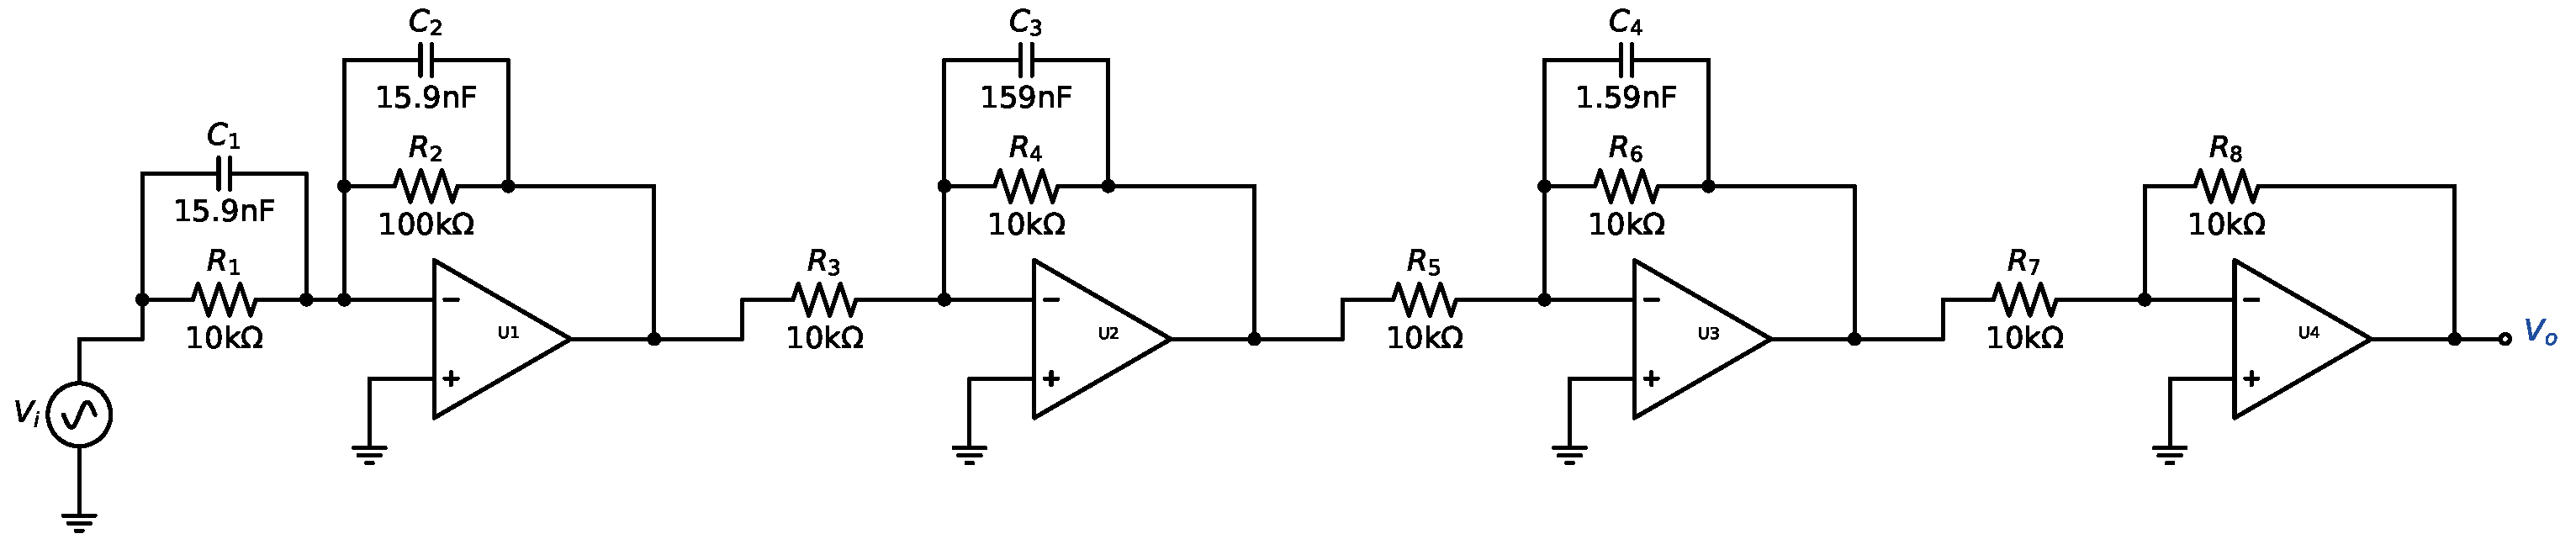
\includegraphics[width=\linewidth,height=5.5cm,keepaspectratio]{p16_design}\end{center}
Check: the stage gains multiply to $(-1)^{4}\cdot10\cdot(\text{factors}) = H(s)$; an independent nodal solve of this circuit reproduces $H(s)$ at every frequency. (Standard-value resistors and capacitors would move the corners slightly.)

The input is $V_i(t) = 0.1\sin\left(2\pi\cdot 300\,t\right)$, so $\omega_{in} = 2\pi\cdot 300 = 1880$\,rad/s. Put $s=j\omega_{in}$ in each factor (tool T5): magnitudes multiply, angles add.
{\small Rules: $\left|\frac{s}{s+p}\right| = \frac{\omega}{\sqrt{\omega^2+p^2}}$, $\angle = \frac{\pi}{2}-\tan^{-1}\frac{\omega}{p}$;\quad $\left|\frac{1}{1+s/p}\right| = \frac{1}{\sqrt{1+(\omega/p)^2}}$, $\angle = -\tan^{-1}\frac{\omega}{p}$;\quad $\left|1+\frac{s}{z}\right| = \sqrt{1+(\omega/z)^2}$, $\angle = \tan^{-1}\frac{\omega}{z}$;\quad a negative $K$ adds $-\pi$.}
\begin{center}\renewcommand{\arraystretch}{1.35}
\begin{tabular}{ccc}
\toprule
factor & magnitude & angle (rad) \\
\midrule
$10$ & $10$ & $0$ \\
$\rule[-1.7em]{0pt}{4em}\dfrac{1}{1+\dfrac{s}{2\pi\cdot 100}}$ & $0.3162$ & $-1.25$ \\
$\rule[-1.7em]{0pt}{4em}\dfrac{1}{1+\dfrac{s}{2\pi\cdot 100}}$ & $0.3162$ & $-1.25$ \\
$\rule[-1.1em]{0pt}{2.8em}\left(1+\dfrac{s}{2\pi\cdot 1\mathrm{k}}\right)$ & $1.044$ & $0.291$ \\
$\rule[-1.7em]{0pt}{4em}\dfrac{1}{1+\dfrac{s}{2\pi\cdot 10\mathrm{k}}}$ & $0.9996$ & $-0.03$ \\
\textbf{total} & $\mathbf{1.044}$ (product) & $\mathbf{-2.24}$ (sum) \\
\bottomrule
\end{tabular}\end{center}

\begin{align*}
|H(j\omega_{in})| &= 1.04, \qquad \angle H(j\omega_{in}) = -2.24\ \mathrm{rad} \\
v_{o,ac}(t) &= 1.04\times 0.1\,\sin\left(2\pi\cdot 300\,t - 2.24\right) = 0.104\,\sin\left(2\pi\cdot 300\,t - 2.24\right)
\end{align*}

\[
\boxed{V_o(t) = 0.104\,\sin\left(2\pi\cdot 300\,t - 2.24\right)\ \mathrm{V}}
\]

\begin{ansbox}
$H(s) = 10\,\dfrac{1}{1+\dfrac{s}{2\pi\cdot 100}}\,\dfrac{1}{1+\dfrac{s}{2\pi\cdot 100}}\,\left(1+\dfrac{s}{2\pi\cdot 1\mathrm{k}}\right)\,\dfrac{1}{1+\dfrac{s}{2\pi\cdot 10\mathrm{k}}}$\\[4pt]
U1: R1 = 10k$\Omega$, C1 = 15.9nF, R2 = 100k$\Omega$, C2 = 15.9nF\\
U2: R3 = 10k$\Omega$, R4 = 10k$\Omega$, C3 = 159nF\\
U3: R5 = 10k$\Omega$, R6 = 10k$\Omega$, C4 = 1.59nF\\
U4: R7 = 10k$\Omega$, R8 = 10k$\Omega$\\[4pt]
$V_o(t) = 0.104\,\sin\left(2\pi\cdot 300\,t - 2.24\right)\ \mathrm{V}$
\end{ansbox}

\newpage
\subsection*{Solution 2C.17 \hfill Hard}
\begin{center}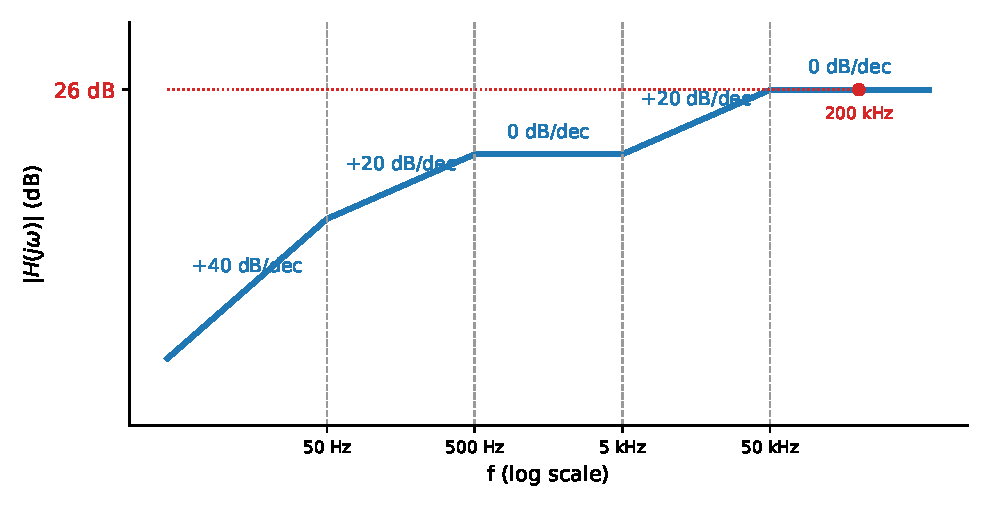
\includegraphics[width=\linewidth,height=5cm,keepaspectratio]{p17_plot}\end{center}
\solstep{1}{Read the corners and slopes}Go left to right along the plot and write down the slope of every straight segment. At each corner frequency the slope changes by a multiple of 20\,dB/dec: every $-20$ is one pole, every $+20$ is one zero (tool T6 read backwards).\begin{center}\renewcommand{\arraystretch}{1.35}
\begin{tabular}{ccccl}
\toprule
corner $f_c$ & slope before & slope after & change & meaning \\
\midrule
50 Hz & $+40$ & $+20$ & $-20$ & one pole at $f_c$ \\
500 Hz & $+20$ & $0$ & $-20$ & one pole at $f_c$ \\
5 kHz & $0$ & $+20$ & $+20$ & one zero at $f_c$ \\
50 kHz & $+20$ & $0$ & $-20$ & one pole at $f_c$ \\
\bottomrule
\end{tabular}\end{center}

\solstep{2}{Starting slope $\Rightarrow$ factors of $s$}The plot starts with a slope of $+40$\,dB/dec, i.e. $|H|\propto\omega^2$ at low frequency: the numerator contains $s^2$. As in class, pair each $s$ with one of the \emph{lowest} poles (50 Hz, 500 Hz) as $\frac{s}{s+p}$: such a factor rises at $+20$\,dB/dec below $p$ and is $\approx1$ (0\,dB) above it. The remaining poles are written $\frac{1}{1+s/p}$ and the zeros $\left(1+\frac{s}{z}\right)$. Every corner is an angular frequency $\omega_c=2\pi f_c$.
\solstep{3}{Assemble $H(s)$}Put one factor per pole/zero in front of an unknown constant $K$:\[
H(s) = K\,\dfrac{s}{s+2\pi\cdot 50}\,\dfrac{s}{s+2\pi\cdot 500}\,\left(1+\dfrac{s}{2\pi\cdot 5\mathrm{k}}\right)\,\dfrac{1}{1+\dfrac{s}{2\pi\cdot 50\mathrm{k}}}
\]

\solstep{4}{Find $K$ from the marked level}The plot marks the level $26$\,dB at $f=$\,200 kHz. On the straight-line plot every factor is either exactly 0\,dB (where it is $\approx1$) or a $\pm20$\,dB/dec line, so evaluate the \emph{asymptote} of each factor at that frequency (the level of a line with slope $\pm20$\,dB/dec is $\pm20\log_{10}(f/f_c)$):\begin{center}\renewcommand{\arraystretch}{1.35}
\begin{tabular}{cccc}
\toprule
factor & $f_c$ & at $f=$\,200 kHz & asymptote (dB) \\
\midrule
$\rule[-1.1em]{0pt}{2.8em}\dfrac{s}{s+2\pi\cdot 50}$ & 50 Hz & $f>f_c$: $\approx 1$ & $0$ \\
$\rule[-1.1em]{0pt}{2.8em}\dfrac{s}{s+2\pi\cdot 500}$ & 500 Hz & $f>f_c$: $\approx 1$ & $0$ \\
$\rule[-1.1em]{0pt}{2.8em}\left(1+\dfrac{s}{2\pi\cdot 5\mathrm{k}}\right)$ & 5 kHz & $f>f_c$: $\approx \frac{\omega}{z}$ & $32$ \\
$\rule[-1.7em]{0pt}{4em}\dfrac{1}{1+\dfrac{s}{2\pi\cdot 50\mathrm{k}}}$ & 50 kHz & $f>f_c$: $\approx \frac{p}{\omega}$ & $-12$ \\
\textbf{sum} &  &  & $\mathbf{20}$ \\
\bottomrule
\end{tabular}\end{center}
The dB values of the factors \emph{add} (magnitudes multiply), so\[
20\log_{10}K = 26 - (20) = 6\ \mathrm{dB}\quad\Rightarrow\quad K = 10^{6/20} = 2
\]

So\[
\boxed{H(s) = 2\,\dfrac{s}{s+2\pi\cdot 50}\,\dfrac{s}{s+2\pi\cdot 500}\,\left(1+\dfrac{s}{2\pi\cdot 5\mathrm{k}}\right)\,\dfrac{1}{1+\dfrac{s}{2\pi\cdot 50\mathrm{k}}}}
\]


\solstep{5}{Split $H(s)$ into op-amp stages}Every inverting stage of the form $-\frac{Z_f}{Z_{in}}$ with $Z_{in}$, $Z_f$ made of one R and at most one C realizes \emph{one} pole, optionally with one zero or one $s$ (tool T2). Pair each zero with a low-pass pole (pole-zero stage), each $\frac{s}{s+p}$ with a remaining low-pass pole (band-pass stage), and give every leftover factor its own stage. Put all of $|K|$ into the first stage. Each stage inverts, so with an odd number of stages add a unity-gain inverter to make $K>0$.\begin{center}\renewcommand{\arraystretch}{1.35}
\begin{tabular}{cccl}
\toprule
stage & gain $\frac{R_2}{R_1}$ & factor(s) realized & block \\
\midrule
U1 & $1.995$ & $\rule[-1.4em]{0pt}{3.4em}\dfrac{s}{s+2\pi\cdot 50}$ & high-pass: $Z_{in}=R+\frac{1}{sC}$, $Z_f=R$ \\
U2 & $1$ & $\rule[-1.4em]{0pt}{3.4em}\dfrac{s}{s+2\pi\cdot 500}$ & high-pass: $Z_{in}=R+\frac{1}{sC}$, $Z_f=R$ \\
U3 & $1$ & $\rule[-1.4em]{0pt}{3.4em}\dfrac{1+\frac{s}{2\pi\cdot 5\mathrm{k}}}{1+\frac{s}{2\pi\cdot 50\mathrm{k}}}$ & pole-zero: $Z_{in}=R\parallel C$, $Z_f = R\parallel C$ \\
U4 & $1$ & $\rule[-1.4em]{0pt}{3.4em}1$ & unity inverter (fixes the sign) \\
\bottomrule
\end{tabular}\end{center}

\solstep{6}{Component values}Use $R_1 = 10\,\mathrm{k}\Omega$ at the input of every stage (any convenient value works; it only scales the other parts). The corner of a factor $1+s/\omega_c$ is matched by $RC = 1/\omega_c$ (corners in rad/s).\begin{enumerate}[leftmargin=*,itemsep=2pt]
\item U1: choose $R_{1} = 10\,\mathrm{k}\Omega$, then match the stage formula $-\frac{R_{2}}{R_{1}}\cdot\frac{s}{s+1/(R_{1}C_{1})}$ to the factors:\[
C_{1} = \frac{1}{314\,R_{1}} = 318\,\mathrm{n}\mathrm{F},\qquad R_{2} = 1.995\,R_{1} = 20\,\mathrm{k}\Omega
\]

\item U2: choose $R_{3} = 10\,\mathrm{k}\Omega$, then match the stage formula $-\frac{R_{4}}{R_{3}}\cdot\frac{s}{s+1/(R_{3}C_{2})}$ to the factors:\[
C_{2} = \frac{1}{3140\,R_{3}} = 31.8\,\mathrm{n}\mathrm{F},\qquad R_{4} = 1\,R_{3} = 10\,\mathrm{k}\Omega
\]

\item U3: choose $R_{5} = 10\,\mathrm{k}\Omega$, then match the stage formula $-\frac{R_{6}}{R_{5}}\cdot\frac{1+sR_{5}C_{3}}{1+sR_{6}C_{4}}$ to the factors:\[
R_{6} = 1\,R_{5} = 10\,\mathrm{k}\Omega,\qquad C_{3} = \frac{1}{31400\,R_{5}} = 3.18\,\mathrm{n}\mathrm{F},\qquad C_{4} = \frac{1}{3.14\times 10^{5}\,R_{6}} = 318\,\mathrm{p}\mathrm{F}
\]

\item U4: $R_{7} = R_{8} = 10\,\mathrm{k}\Omega$ (gain $-1$).
\end{enumerate}

\solstep{7}{Check and steady-state output}The designed circuit:\begin{center}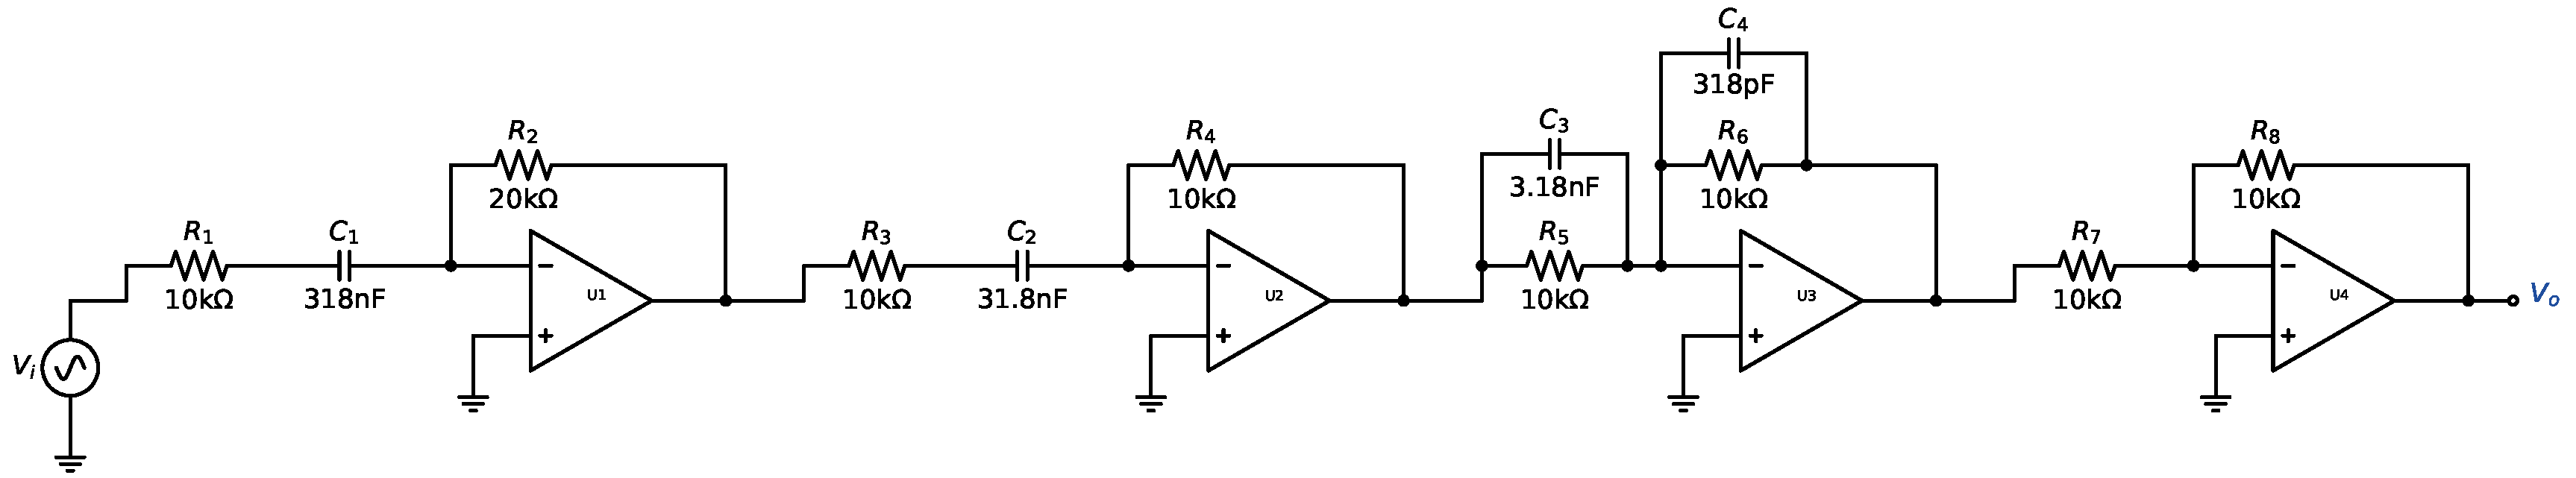
\includegraphics[width=\linewidth,height=5.5cm,keepaspectratio]{p17_design}\end{center}
Check: the stage gains multiply to $(-1)^{4}\cdot1.995\cdot(\text{factors}) = H(s)$; an independent nodal solve of this circuit reproduces $H(s)$ at every frequency. (Standard-value resistors and capacitors would move the corners slightly.)

The input is $V_i(t) = 0.05\cos\left(2\pi\cdot 1000\,t-\frac{\pi}{6}\right)$, so $\omega_{in} = 2\pi\cdot 1000 = 6280$\,rad/s. Put $s=j\omega_{in}$ in each factor (tool T5): magnitudes multiply, angles add.
{\small Rules: $\left|\frac{s}{s+p}\right| = \frac{\omega}{\sqrt{\omega^2+p^2}}$, $\angle = \frac{\pi}{2}-\tan^{-1}\frac{\omega}{p}$;\quad $\left|\frac{1}{1+s/p}\right| = \frac{1}{\sqrt{1+(\omega/p)^2}}$, $\angle = -\tan^{-1}\frac{\omega}{p}$;\quad $\left|1+\frac{s}{z}\right| = \sqrt{1+(\omega/z)^2}$, $\angle = \tan^{-1}\frac{\omega}{z}$;\quad a negative $K$ adds $-\pi$.}
\begin{center}\renewcommand{\arraystretch}{1.35}
\begin{tabular}{ccc}
\toprule
factor & magnitude & angle (rad) \\
\midrule
$2$ & $1.995$ & $0$ \\
$\rule[-1.1em]{0pt}{2.8em}\dfrac{s}{s+2\pi\cdot 50}$ & $0.9988$ & $0.05$ \\
$\rule[-1.1em]{0pt}{2.8em}\dfrac{s}{s+2\pi\cdot 500}$ & $0.8944$ & $0.464$ \\
$\rule[-1.1em]{0pt}{2.8em}\left(1+\dfrac{s}{2\pi\cdot 5\mathrm{k}}\right)$ & $1.02$ & $0.197$ \\
$\rule[-1.7em]{0pt}{4em}\dfrac{1}{1+\dfrac{s}{2\pi\cdot 50\mathrm{k}}}$ & $0.9998$ & $-0.02$ \\
\textbf{total} & $\mathbf{1.817}$ (product) & $\mathbf{0.691}$ (sum) \\
\bottomrule
\end{tabular}\end{center}

\begin{align*}
|H(j\omega_{in})| &= 1.82, \qquad \angle H(j\omega_{in}) = 0.691\ \mathrm{rad} \\
v_{o,ac}(t) &= 1.82\times 0.05\,\cos\left(2\pi\cdot 1000\,t + 0.167\right) = 0.0909\,\cos\left(2\pi\cdot 1000\,t + 0.167\right)
\end{align*}

(phase: $\theta + \angle H = -\frac{\pi}{6} + (0.691) = 0.167$\,rad.)
\[
\boxed{V_o(t) = 0.0909\,\cos\left(2\pi\cdot 1000\,t + 0.167\right)\ \mathrm{V}}
\]

\begin{ansbox}
$H(s) = 2\,\dfrac{s}{s+2\pi\cdot 50}\,\dfrac{s}{s+2\pi\cdot 500}\,\left(1+\dfrac{s}{2\pi\cdot 5\mathrm{k}}\right)\,\dfrac{1}{1+\dfrac{s}{2\pi\cdot 50\mathrm{k}}}$\\[4pt]
U1: R1 = 10k$\Omega$, C1 = 318nF, R2 = 20k$\Omega$\\
U2: R3 = 10k$\Omega$, C2 = 31.8nF, R4 = 10k$\Omega$\\
U3: R5 = 10k$\Omega$, C3 = 3.18nF, R6 = 10k$\Omega$, C4 = 318pF\\
U4: R7 = 10k$\Omega$, R8 = 10k$\Omega$\\[4pt]
$V_o(t) = 0.0909\,\cos\left(2\pi\cdot 1000\,t + 0.167\right)\ \mathrm{V}$
\end{ansbox}

\newpage
\subsection*{Solution 2C.18 \hfill Hard}
\begin{center}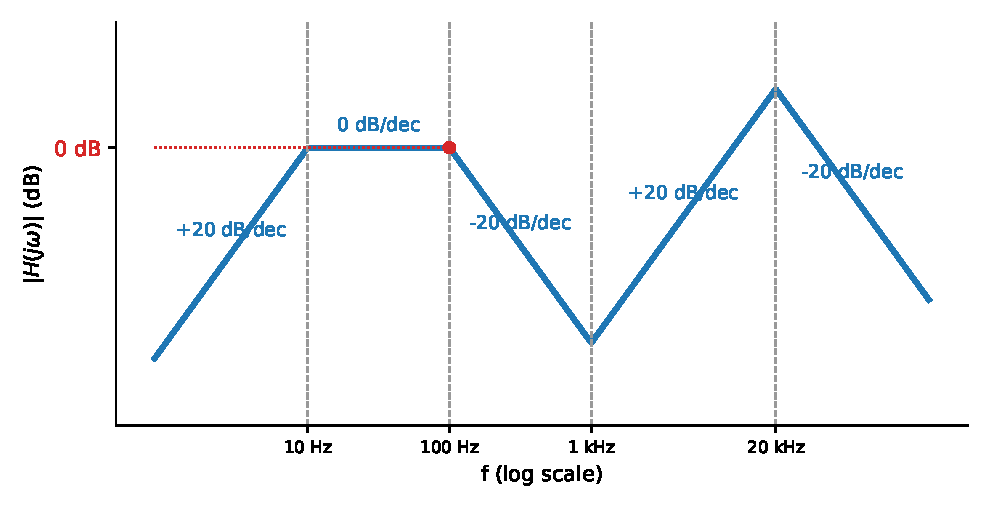
\includegraphics[width=\linewidth,height=5cm,keepaspectratio]{p18_plot}\end{center}
\solstep{1}{Read the corners and slopes}Go left to right along the plot and write down the slope of every straight segment. At each corner frequency the slope changes by a multiple of 20\,dB/dec: every $-20$ is one pole, every $+20$ is one zero (tool T6 read backwards).\begin{center}\renewcommand{\arraystretch}{1.35}
\begin{tabular}{ccccl}
\toprule
corner $f_c$ & slope before & slope after & change & meaning \\
\midrule
10 Hz & $+20$ & $0$ & $-20$ & one pole at $f_c$ \\
100 Hz & $0$ & $-20$ & $-20$ & one pole at $f_c$ \\
1 kHz & $-20$ & $+20$ & $+40$ & two zeros at $f_c$ \\
20 kHz & $+20$ & $-20$ & $-40$ & two poles at $f_c$ \\
\bottomrule
\end{tabular}\end{center}

\solstep{2}{Starting slope $\Rightarrow$ factors of $s$}The plot starts with a slope of $+20$\,dB/dec, i.e. $|H|\propto\omega^1$ at low frequency: the numerator contains $s$. As in class, pair each $s$ with one of the \emph{lowest} poles (10 Hz) as $\frac{s}{s+p}$: such a factor rises at $+20$\,dB/dec below $p$ and is $\approx1$ (0\,dB) above it. The remaining poles are written $\frac{1}{1+s/p}$ and the zeros $\left(1+\frac{s}{z}\right)$. Every corner is an angular frequency $\omega_c=2\pi f_c$.
\solstep{3}{Assemble $H(s)$}Put one factor per pole/zero in front of an unknown constant $K$:\[
H(s) = K\,\dfrac{s}{s+2\pi\cdot 10}\,\dfrac{1}{1+\dfrac{s}{2\pi\cdot 100}}\,\left(1+\dfrac{s}{2\pi\cdot 1\mathrm{k}}\right)\,\left(1+\dfrac{s}{2\pi\cdot 1\mathrm{k}}\right)\,\dfrac{1}{1+\dfrac{s}{2\pi\cdot 20\mathrm{k}}}\,\dfrac{1}{1+\dfrac{s}{2\pi\cdot 20\mathrm{k}}}
\]

\solstep{4}{Find $K$ from the marked level}The plot marks the level $0$\,dB at $f=$\,100 Hz. On the straight-line plot every factor is either exactly 0\,dB (where it is $\approx1$) or a $\pm20$\,dB/dec line, so evaluate the \emph{asymptote} of each factor at that frequency (the level of a line with slope $\pm20$\,dB/dec is $\pm20\log_{10}(f/f_c)$):\begin{center}\renewcommand{\arraystretch}{1.35}
\begin{tabular}{cccc}
\toprule
factor & $f_c$ & at $f=$\,100 Hz & asymptote (dB) \\
\midrule
$\rule[-1.1em]{0pt}{2.8em}\dfrac{s}{s+2\pi\cdot 10}$ & 10 Hz & $f>f_c$: $\approx 1$ & $0$ \\
$\rule[-1.7em]{0pt}{4em}\dfrac{1}{1+\dfrac{s}{2\pi\cdot 100}}$ & 100 Hz & $f<f_c$: $\approx 1$ & $0$ \\
$\rule[-1.1em]{0pt}{2.8em}\left(1+\dfrac{s}{2\pi\cdot 1\mathrm{k}}\right)$ & 1 kHz & $f<f_c$: $\approx 1$ & $0$ \\
$\rule[-1.1em]{0pt}{2.8em}\left(1+\dfrac{s}{2\pi\cdot 1\mathrm{k}}\right)$ & 1 kHz & $f<f_c$: $\approx 1$ & $0$ \\
$\rule[-1.7em]{0pt}{4em}\dfrac{1}{1+\dfrac{s}{2\pi\cdot 20\mathrm{k}}}$ & 20 kHz & $f<f_c$: $\approx 1$ & $0$ \\
$\rule[-1.7em]{0pt}{4em}\dfrac{1}{1+\dfrac{s}{2\pi\cdot 20\mathrm{k}}}$ & 20 kHz & $f<f_c$: $\approx 1$ & $0$ \\
\textbf{sum} &  &  & $\mathbf{0}$ \\
\bottomrule
\end{tabular}\end{center}
The dB values of the factors \emph{add} (magnitudes multiply), so\[
20\log_{10}K = 0 - (0) = 0\ \mathrm{dB}\quad\Rightarrow\quad K = 10^{0/20} = 1
\]

So\[
\boxed{H(s) = 1\,\dfrac{s}{s+2\pi\cdot 10}\,\dfrac{1}{1+\dfrac{s}{2\pi\cdot 100}}\,\left(1+\dfrac{s}{2\pi\cdot 1\mathrm{k}}\right)\,\left(1+\dfrac{s}{2\pi\cdot 1\mathrm{k}}\right)\,\dfrac{1}{1+\dfrac{s}{2\pi\cdot 20\mathrm{k}}}\,\dfrac{1}{1+\dfrac{s}{2\pi\cdot 20\mathrm{k}}}}
\]


\solstep{5}{Split $H(s)$ into op-amp stages}Every inverting stage of the form $-\frac{Z_f}{Z_{in}}$ with $Z_{in}$, $Z_f$ made of one R and at most one C realizes \emph{one} pole, optionally with one zero or one $s$ (tool T2). Pair each zero with a low-pass pole (pole-zero stage), each $\frac{s}{s+p}$ with a remaining low-pass pole (band-pass stage), and give every leftover factor its own stage. Put all of $|K|$ into the first stage. Each stage inverts, so with an odd number of stages add a unity-gain inverter to make $K>0$.\begin{center}\renewcommand{\arraystretch}{1.35}
\begin{tabular}{cccl}
\toprule
stage & gain $\frac{R_2}{R_1}$ & factor(s) realized & block \\
\midrule
U1 & $1$ & $\rule[-1.4em]{0pt}{3.4em}\dfrac{s}{s+2\pi\cdot 10}\cdot\dfrac{1}{1+\frac{s}{2\pi\cdot 20\mathrm{k}}}$ & band-pass: $Z_{in}=R+\frac{1}{sC}$, $Z_f=R\parallel C$ \\
U2 & $1$ & $\rule[-1.4em]{0pt}{3.4em}\dfrac{1+\frac{s}{2\pi\cdot 1\mathrm{k}}}{1+\frac{s}{2\pi\cdot 100}}$ & pole-zero: $Z_{in}=R\parallel C$, $Z_f = R\parallel C$ \\
U3 & $1$ & $\rule[-1.4em]{0pt}{3.4em}\dfrac{1+\frac{s}{2\pi\cdot 1\mathrm{k}}}{1+\frac{s}{2\pi\cdot 20\mathrm{k}}}$ & pole-zero: $Z_{in}=R\parallel C$, $Z_f = R\parallel C$ \\
U4 & $1$ & $\rule[-1.4em]{0pt}{3.4em}1$ & unity inverter (fixes the sign) \\
\bottomrule
\end{tabular}\end{center}

\solstep{6}{Component values}Use $R_1 = 10\,\mathrm{k}\Omega$ at the input of every stage (any convenient value works; it only scales the other parts). The corner of a factor $1+s/\omega_c$ is matched by $RC = 1/\omega_c$ (corners in rad/s).\begin{enumerate}[leftmargin=*,itemsep=2pt]
\item U1: choose $R_{1} = 10\,\mathrm{k}\Omega$, then match the stage formula $-\frac{R_{2}}{R_{1}}\cdot\frac{s}{s+1/(R_{1}C_{1})}\cdot\frac{1}{1+sR_{2}C_{2}}$ to the factors:\[
C_{1} = \frac{1}{62.8\,R_{1}} = 1.59\,\mu \mathrm{F},\qquad R_{2} = 1\,R_{1} = 10\,\mathrm{k}\Omega,\qquad C_{2} = \frac{1}{1.26\times 10^{5}\,R_{2}} = 796\,\mathrm{p}\mathrm{F}
\]

\item U2: choose $R_{3} = 10\,\mathrm{k}\Omega$, then match the stage formula $-\frac{R_{4}}{R_{3}}\cdot\frac{1+sR_{3}C_{3}}{1+sR_{4}C_{4}}$ to the factors:\[
R_{4} = 1\,R_{3} = 10\,\mathrm{k}\Omega,\qquad C_{3} = \frac{1}{6280\,R_{3}} = 15.9\,\mathrm{n}\mathrm{F},\qquad C_{4} = \frac{1}{628\,R_{4}} = 159\,\mathrm{n}\mathrm{F}
\]

\item U3: choose $R_{5} = 10\,\mathrm{k}\Omega$, then match the stage formula $-\frac{R_{6}}{R_{5}}\cdot\frac{1+sR_{5}C_{5}}{1+sR_{6}C_{6}}$ to the factors:\[
R_{6} = 1\,R_{5} = 10\,\mathrm{k}\Omega,\qquad C_{5} = \frac{1}{6280\,R_{5}} = 15.9\,\mathrm{n}\mathrm{F},\qquad C_{6} = \frac{1}{1.26\times 10^{5}\,R_{6}} = 796\,\mathrm{p}\mathrm{F}
\]

\item U4: $R_{7} = R_{8} = 10\,\mathrm{k}\Omega$ (gain $-1$).
\end{enumerate}

\solstep{7}{Check and steady-state output}The designed circuit:\begin{center}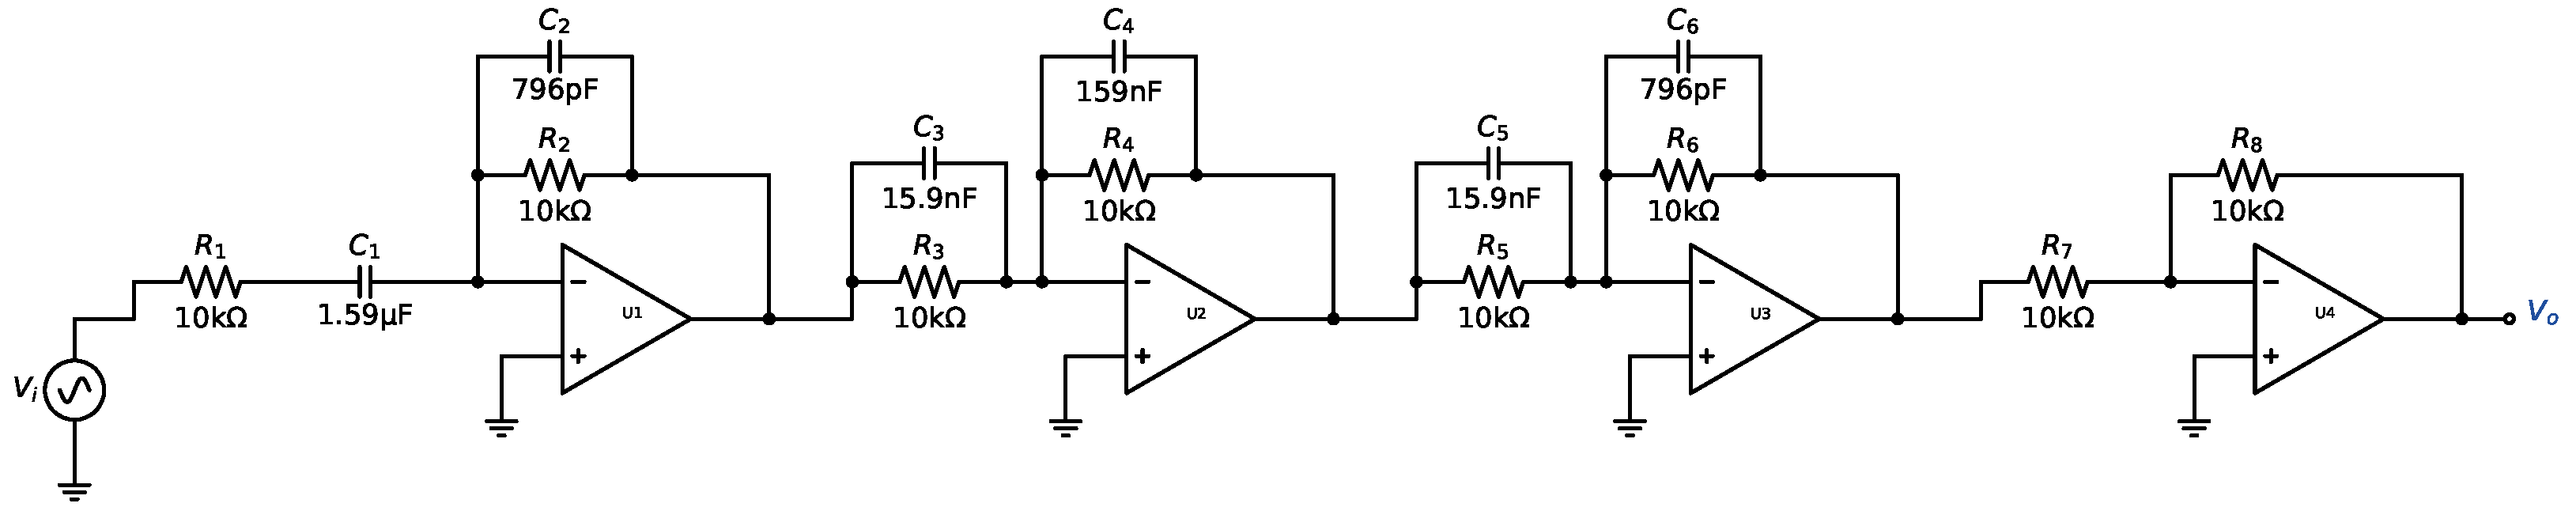
\includegraphics[width=\linewidth,height=5.5cm,keepaspectratio]{p18_design}\end{center}
Check: the stage gains multiply to $(-1)^{4}\cdot1\cdot(\text{factors}) = H(s)$; an independent nodal solve of this circuit reproduces $H(s)$ at every frequency. (Standard-value resistors and capacitors would move the corners slightly.)

The input is $V_i(t) = 0.5\sin\left(2\pi\cdot 3000\,t\right)$, so $\omega_{in} = 2\pi\cdot 3000 = 18800$\,rad/s. Put $s=j\omega_{in}$ in each factor (tool T5): magnitudes multiply, angles add.
{\small Rules: $\left|\frac{s}{s+p}\right| = \frac{\omega}{\sqrt{\omega^2+p^2}}$, $\angle = \frac{\pi}{2}-\tan^{-1}\frac{\omega}{p}$;\quad $\left|\frac{1}{1+s/p}\right| = \frac{1}{\sqrt{1+(\omega/p)^2}}$, $\angle = -\tan^{-1}\frac{\omega}{p}$;\quad $\left|1+\frac{s}{z}\right| = \sqrt{1+(\omega/z)^2}$, $\angle = \tan^{-1}\frac{\omega}{z}$;\quad a negative $K$ adds $-\pi$.}
\begin{center}\renewcommand{\arraystretch}{1.35}
\begin{tabular}{ccc}
\toprule
factor & magnitude & angle (rad) \\
\midrule
$1$ & $1$ & $0$ \\
$\rule[-1.1em]{0pt}{2.8em}\dfrac{s}{s+2\pi\cdot 10}$ & $1$ & $0.00333$ \\
$\rule[-1.7em]{0pt}{4em}\dfrac{1}{1+\dfrac{s}{2\pi\cdot 100}}$ & $0.03331$ & $-1.54$ \\
$\rule[-1.1em]{0pt}{2.8em}\left(1+\dfrac{s}{2\pi\cdot 1\mathrm{k}}\right)$ & $3.162$ & $1.25$ \\
$\rule[-1.1em]{0pt}{2.8em}\left(1+\dfrac{s}{2\pi\cdot 1\mathrm{k}}\right)$ & $3.162$ & $1.25$ \\
$\rule[-1.7em]{0pt}{4em}\dfrac{1}{1+\dfrac{s}{2\pi\cdot 20\mathrm{k}}}$ & $0.9889$ & $-0.149$ \\
$\rule[-1.7em]{0pt}{4em}\dfrac{1}{1+\dfrac{s}{2\pi\cdot 20\mathrm{k}}}$ & $0.9889$ & $-0.149$ \\
\textbf{total} & $\mathbf{0.3258}$ (product) & $\mathbf{0.666}$ (sum) \\
\bottomrule
\end{tabular}\end{center}

\begin{align*}
|H(j\omega_{in})| &= 0.326, \qquad \angle H(j\omega_{in}) = 0.666\ \mathrm{rad} \\
v_{o,ac}(t) &= 0.326\times 0.5\,\sin\left(2\pi\cdot 3000\,t + 0.666\right) = 0.163\,\sin\left(2\pi\cdot 3000\,t + 0.666\right)
\end{align*}

\[
\boxed{V_o(t) = 0.163\,\sin\left(2\pi\cdot 3000\,t + 0.666\right)\ \mathrm{V}}
\]

\begin{ansbox}
$H(s) = 1\,\dfrac{s}{s+2\pi\cdot 10}\,\dfrac{1}{1+\dfrac{s}{2\pi\cdot 100}}\,\left(1+\dfrac{s}{2\pi\cdot 1\mathrm{k}}\right)\,\left(1+\dfrac{s}{2\pi\cdot 1\mathrm{k}}\right)\,\dfrac{1}{1+\dfrac{s}{2\pi\cdot 20\mathrm{k}}}\,\dfrac{1}{1+\dfrac{s}{2\pi\cdot 20\mathrm{k}}}$\\[4pt]
U1: R1 = 10k$\Omega$, C1 = 1.59$\mu$F, R2 = 10k$\Omega$, C2 = 796pF\\
U2: R3 = 10k$\Omega$, C3 = 15.9nF, R4 = 10k$\Omega$, C4 = 159nF\\
U3: R5 = 10k$\Omega$, C5 = 15.9nF, R6 = 10k$\Omega$, C6 = 796pF\\
U4: R7 = 10k$\Omega$, R8 = 10k$\Omega$\\[4pt]
$V_o(t) = 0.163\,\sin\left(2\pi\cdot 3000\,t + 0.666\right)\ \mathrm{V}$
\end{ansbox}

\end{document}
